\documentclass[12pt]{article}
\usepackage[margin=1in]{geometry}
\usepackage[T1]{fontenc}
\usepackage[utf8]{inputenc}
\usepackage{CJKutf8}
\usepackage{lmodern}
\usepackage{setspace}
\usepackage{enumitem}
\usepackage{graphicx}
\usepackage{wrapfig}
\usepackage{hyperref}
\usepackage{tikz}
\usetikzlibrary{arrows.meta,positioning,calc,fit}

\setlength{\parindent}{0pt}
\setlength{\parskip}{0.8\baselineskip}

% Encourage large figures to share pages with text (avoid float-only pages).
\setcounter{topnumber}{2}
\setcounter{bottomnumber}{2}
\setcounter{totalnumber}{4}
\renewcommand{\topfraction}{0.95}
\renewcommand{\bottomfraction}{0.95}
\renewcommand{\textfraction}{0.05}
\renewcommand{\floatpagefraction}{0.95}

\begin{document}
\onehalfspacing

% =========================
% TITLE PAGE
% =========================
\begin{titlepage}
  \centering
  \vspace*{1in}

  {\Large \textbf{SIGNATURE WORK FINAL PAPER}\par}
  \vspace{0.5\baselineskip}
  {(Creative Practice: iOS App Design)\par}

  \vspace{1.5in}

  {\Large \textbf{SIDEQUEST: Full Stack Application Development}\par}
  \vspace{0.5\baselineskip}
  {\large \textit{iOS app design through iterative product principles}\par}

  \vfill
\end{titlepage}

% =========================
% ABSTRACT
% =========================
\section*{ABSTRACT}
SideQuest is a location based photo-challenge app designed to encourage engagement with real-world places through gamification and social interaction. The project addresses a gap in mainstream social media apps: digital posting is rarely tied to physical context, and ``creation'' is often reduced to passive consumption loops. SideQuest uses 'Quest' prompts, location-based photo capture, and meaning-making through gamification to encourage user engagement. The app architecture broadly follows the MERN tech stack, and was developed through iterative user-centered prototyping and formal TestFlight evaluation, combining qualitative feedback and issue tracking. After only a month of release, SideQuest has a dedicated group of 30 daily active users (DAU), enabling continuous app design under real usage conditions. The final product is a first-of-a-kind full stack application available on the App Store, that replaces passive scrolling by enabling users to get out and Quest.


\textbf{Keywords:} product design; full stack development; iterative development; gamification; systems design.

\textbf{Outcome:} A deployed product published to the App Store with scalable system architecture and an active userbase.

\textbf{Contribution:} First-of-a-kind application design of a novel concept and full stack buildout.



% =========================
% ACKNOWLEDGEMENTS
% =========================
\section*{ACKNOWLEDGEMENTS}
First and foremost, I would like to thank my mentor Professor Jiang Long, for his willingness to provide support wherever the development process took us. The success of this project would not have been possible without his consistent support and engagement. Thank you also to my co-founder Michael Cornell, who willingly stayed awake many a late night debugging code (and especially doing battle with the Apple ecosystem). Thanks to Teohan 'Dino' Blind for coming up with the name 'SideQuest', and in doing so finally helping us escape the matrix. Thank you as well to Krishna Thiagarajan, who I view as the user persona for the type of person who loves the app, and who gave endless suggestions in the development process. Finally, thank you to our Beta test users, including Thomas Boyle, Ethan 'Cobbe' Deal, Zoya Hussein Abbas, Kailani Peng Wang, Mason Swayne, Katherine Cornell, and many, many others.

We also acknowledge the valuable work of the many open source tools that made this project possible, including React Native, Expo, Node.js, Express, MongoDB, Mongoose, Docker, Jest, and as always a great deal of special love for Git.

% =========================
% INTRODUCTION
% =========================
\section*{INTRODUCTION}
Most consumer social apps optimize for one thing: keeping you looking at a screen. Photos and short-form content are abundant, but they are broadly damaging and addictive for people who use them (Bucher, 2012; Abidin, 2016), and are rarely designed to make people do anything in the physical world. Location, when it appears at all, is typically treated as passive metadata (a tag), not as an active ingredient that shapes what you create, where you go, and who you meet. At the same time, many location-based apps that do motivate active movement (navigation, reviews) tend to be utility-driven, leaving little room for user-focused creativity. The result is a gap: there are few apps that encourage users to take positive actions in the real world, while also encouraging participation through social gamification.

SideQuest targets that gap. It is built on the idea that seeking discomfort and novelty is the best thing someone can do to enrich their life. SideQuest aims to shift behavior away from passive scrolling and toward sharing social exploration in the real world.

\subsection*{Project Intent: What is SideQuest?}

\begin{wrapfigure}[23]{r}{0.35\textwidth}
  \vspace{-3.7\baselineskip}
  \centering
  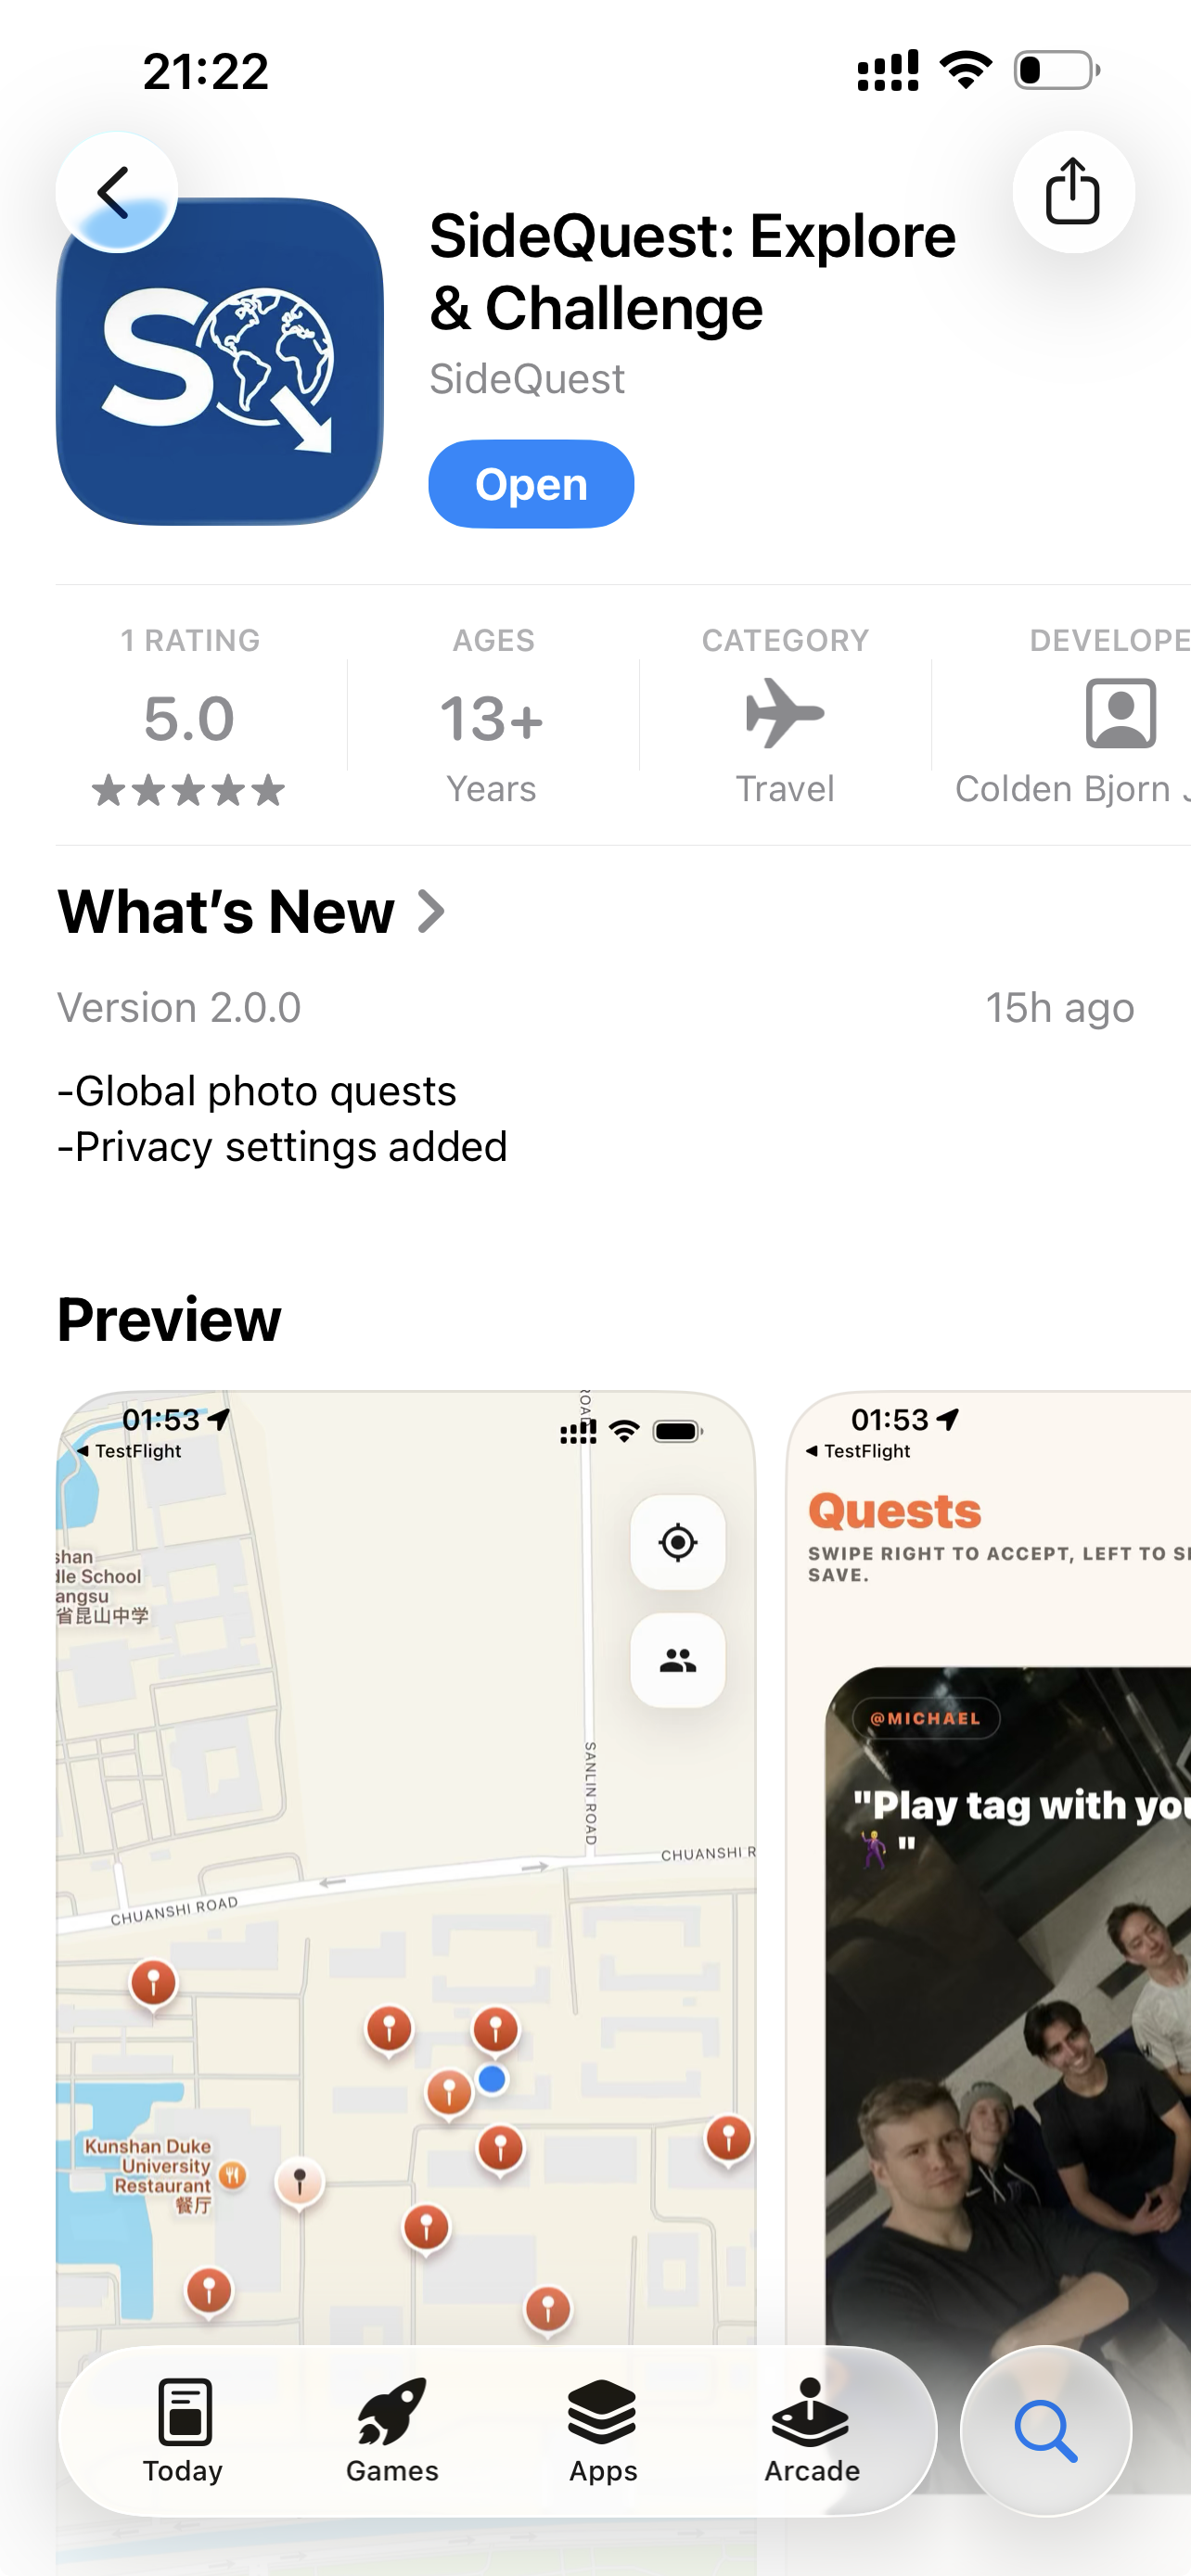
\includegraphics[width=\linewidth]{AppPhotos/sidequest_appstorepage}
  \caption{SideQuest App Store listing.}
  \label{fig:appstore-listing}
  \vspace{-1.0\baselineskip}
\end{wrapfigure}

SideQuest is a location and activity focused photo-challenge app. It encourages creative and novel engagement with real-world places through social gamification.

Users create a new Quest at a map location by snapping a photo and attaching a short prompt. One real user example was 'take a photo with a new friend', accompanied by a photo of the user and a campus \begin{CJK}{UTF8}{gbsn}保安\end{CJK} security guard. Other users then follow that same Quest prompt to contribute their own photos with new friends. On this particular pin, users uploaded photos with everything from other DKU students, to silly pictures of them frowning by themselves. This transforms a given Quest into an evolving, community-built creative artifact. More concretely, it encourages users to take a minute to do something positive in their day: meet a new friend, and share that moment with others.

Other Quests have included prompts like "you in your favorite study spot", "play tag with your friends", "that gym lifestyle", or "best restaurant in Shanghai". All of these Quests encourage a certain type of feeling among users: in interviews, users have reported that SideQuest "encourages me to try new things", and "I go to places and do new things I never would have thought of [without SideQuest]".

To incentivize participation beyond sharing with friends, SideQuest has a gamification system to reward creativity. All submissions are included in head-to-head ``duels'', where users vote by swiping. These outcomes create a (reductively) Elo-style ranking that encourages compelling contributions over time. This voting system highlights top photos to inspire others and gives users unique badges to exhibit on their profiles. SideQuest also allows users to add and directly challenge friends, creating sustained and meaningful engagement.

SideQuest delivers a creative design project along the entire product axis, including full stack development, product design, and Agile methodology-style user testing + integration. The core output is therefore twofold: (1) an App Store-published iOS app with real user base, and (2) a documented creative design and research process with reasoned decision making.

SideQuest is available for download on the App Store \textit{(Fig.~\ref{fig:appstore-listing})}. We encourage readers to download the app on iOS by searching "SideQuest: Explore \& Challenge". Note that a VPN is needed when in China to use the app (including for phone number registration).

\subsection*{Design Philosophy}

SideQuest's UX behavior is developed using a user-centered, iterative philosophy common in modern product design/HCI (Human Computer Interaction). Simply, this approach strives to build prototypes early, test with real users, and ship improvments based on user data, based loosely on the Agile design philosophy (Fig. ~\ref{fig:agile-cycle}). Two beliefs drive this approach:

\begin{itemize}[leftmargin=*, itemsep=0.4\baselineskip]
  \item Design claims must be observable in use. If a mechanic is intended to be motivating but this is not borne out by the data, the mechanic is necessarily wrong (or miscommunicated), regardless of intent.
  \item Late-stage testing is comparatively expensive. Testing is embedded continuously because the cost of fixing fundamental issues balloons in complexity as features accumulate.
\end{itemize}

\begin{figure}[!htbp]
  \centering
  \definecolor{sqorange}{HTML}{FF6B35}
  \definecolor{sqcoral}{HTML}{FFD9CC}
  \definecolor{sqpeach}{HTML}{FFE9D6}
  \definecolor{sqmint}{HTML}{DDF3E4}
  \definecolor{sqsky}{HTML}{DCEEFE}
  \definecolor{sqlav}{HTML}{E9E2FF}
  \definecolor{sqnotea}{HTML}{FFF4EE}
  \definecolor{sqnoteb}{HTML}{EEF7FF}

  \resizebox{\linewidth}{!}{%
  \begin{tikzpicture}[
    font=\sffamily,
    box/.style={draw=sqorange!80!black, text=black, rounded corners=6pt, minimum width=34mm, minimum height=12mm, align=center, line width=0.45pt},
    note/.style={draw=sqorange!65!black, rounded corners=6pt, inner xsep=6pt, inner ysep=4pt, align=left, line width=0.4pt},
    arrow/.style={-Latex, thick, draw=sqorange!85!black},
    node distance=14mm
  ]

  \node[box, fill=sqcoral] (design) {Design};
  \node[box, fill=sqpeach, right=of design] (dev) {Development};
  \node[box, fill=sqmint, right=of dev] (test) {Testing};
  \node[box, fill=sqsky, right=of test] (deploy) {Deployment};
  \node[box, fill=sqlav, right=of deploy] (feedback) {User Feedback};

  \draw[arrow] (design) -- (dev);
  \draw[arrow] (dev) -- (test);
  \draw[arrow] (test) -- (deploy);
  \draw[arrow] (deploy) -- (feedback);

  \draw[arrow] (feedback.south) .. controls +(0,-14mm) and +(0,-14mm) .. (design.south);

  \node[draw=sqorange!70!black, dashed, rounded corners=10pt, fit=(design)(dev)(test)(deploy)(feedback), inner sep=9mm] (sprint) {};
  \node[fill=white, text=sqorange!85!black, inner sep=2pt, font=\bfseries\small] at ([yshift=7mm]sprint.north) {1-week Sprint (repeat weekly)};

  \node[note, fill=sqnotea, below=20mm of test, anchor=north] (testflight) {\textbf{TestFlight with real users}\\
  \footnotesize
  \begin{tabular}{@{}l@{}}
  - User journeys\\
  - Bugs documentation
  \end{tabular}};
  \draw[arrow] (deploy.south) -- ++(0,-6mm) -| (testflight.north);

  \node[note, fill=sqnoteb, below=20mm of feedback, anchor=north] (backlog) {\textbf{Feedback $\rightarrow$ Backlog}\\
  \footnotesize
  \begin{tabular}{@{}l@{}}
  - Shared issue tracking doc \\
  - Prioritize fixes + next features
  \end{tabular}};
  \draw[arrow] (feedback.south) -- ++(0,-6mm) -- (backlog.north);

  \end{tikzpicture}%
  }
  \caption{Agile manifesto-inspired workflow in SideQuest: weekly sprint loop from design to deployment.}
  \label{fig:agile-cycle}
\end{figure}

\subsubsection*{User Feedback Gathering}

To constantly create an updated feature backlog and prioritize issues, we relied mainly on three testing channels:

\begin{itemize}[leftmargin=*, itemsep=0.25\baselineskip]
  \item \textbf{TestFlight with Real Users:} Structured observational sessions map user journeys through the app and pair direct observation with post-session reflection. This process has consistently identified bugs, unintuitive flows, and friction points.
  \item \textbf{Ongoing Qualitative Feedback:} A live feedback document with issue tracking captures recurring complaints, aesthetic critiques, and suggestions. Users are encouraged to text at any time for help with issues or confusion.
  \item \textbf{Deployment Behavioral Validation:} With a stable group of daily active users (DAU), we monitor daily usage of the app to assess 'ecological validity' and guide what features are lacking in subsequent releases.
\end{itemize}

\subsection*{Guiding Questions}
\begin{itemize}[leftmargin=*, itemsep=0.25\baselineskip]
  \item What architecture is required to support a production-grade app published to the App Store?
  \item What does a product manager's role look like, and how should user feedback contribute to the overall design of a product?
  \item To what extent can social gamification incentivize user engagement?
  \item What does modern app development look like, and to what extent can workflows be accelerated (examined from the perspective of CI/CD, AI, Agile iteration, and more)?
  \item What does working in a startup environment feel like, and is this something I would like to explore more in the future?
\end{itemize}

\subsection*{Technical Architecture}
SideQuest's technical architecture is by far the most time-consuming aspect of the project, and significant effort goes into publishing a reliable, secure, and bug-free app to the App Store. For the technically inclined reader, an introductory overview is included here, and discussed in more detail in subsequent sections. \textit{(Fig.~\ref{fig:system-architecture})}:

\begin{itemize}[leftmargin=*, itemsep=0.25\baselineskip]
  \item Client: React Native Expo, iOS-first distribution via TestFlight (also buildable for Android distribution)
  \item Backend: MERN-style stack (Node.js + Express + MongoDB with Mongoose)
  \item Auth: Firebase Authentication (email/password and phone/SMS), with server-side verification
  \item Photo storage: Firebase storage with URIs tied to pin data in MongoDB
  \item Deployment: Dockerized backend deployed on Google Cloud Run (GCR)
  \item Testing: Postman for endpoint validation Jest for unit testing
  \item CI/CD Pipeline: Integrated on both Google Cloud Run and XCode Cloud
  \item Git: Important for versioning, Agile methodologies, and collaborating with team members
\end{itemize}

\begin{figure}[!htbp]
  \centering
  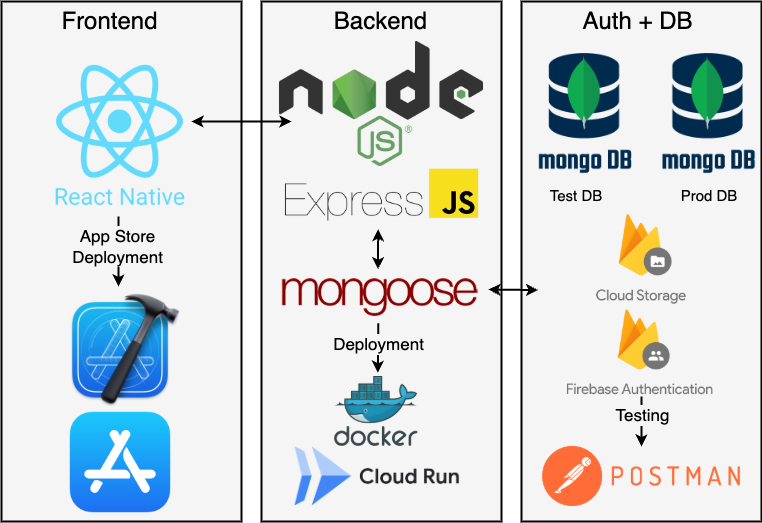
\includegraphics[width=0.95\linewidth]{SideQuestArchitectureDiagram.png}
  \caption{System architecture diagram. \textit{(High-level view of SideQuest key services)}}
  \label{fig:system-architecture}
\end{figure}

% TODO: Make a simplified diagram for up here and a detailed one for the technical methods section.


\subsection*{Significance}
This project is significant for three main reasons. First, it explores a novel app concept aimed at freeing users from passive consumption loops pervasive in modern society. This claim is supported by early adoption and continued use among a group of active users.

Technically, the project delivers a production-grade full-stack architecture capable of supporting a real App Store product. Successful deployment of this nature is exceedingly rare for a signature work product, and demonstrates technical competence across mobile development, backend systems, databases, and frontend UI design.

Finally, it demonstrates practical product leadership, following a user-centered Agile workflow. Successful execution of this project mirrors the role of a technical Product Manager (PM) in modern software teams.


% =========================
% MEDIA AND LITERATURE REVIEW
% =========================
\section*{MEDIA AND LITERATURE REVIEW}
\subsection*{Overview}
This review establishes the conceptual and practical foundation for SideQuest by examining prior work in location-based media, social photo-sharing platforms, gamification and social comparison, and iterative, user-centered design practices. Rather than surveying all adjacent domains, this review focuses on precedents that directly inform the project's core claim: that encouraging creative participation in a specific physical place encourages active engagement over passive consumption. Each subsection concludes with some concrete implications for product design.

\subsection*{1.\ Location-based media and situated interaction}
\subsubsection*{Historical and conceptual grounding}
When searching for an artistic and philosophical grounding for the project, research on location-based media emphasizes the idea of 'situated interaction': digital content that gains meaning \textit{from} its physical context. For example, Pok\'emon GO requires players to travel through the environment to interact with various on-screen elements. In this way, the surrounding landscape becomes part of the game's narrative. Mobile media research argues that location can act as a narrative or experiental addition that reshapes and amplifies user behavior (Hemment, 2006; de Souza e Silva \& Sutko, 2009).

\textbf{Design implication:} Location should amplify interaction, acting as either a gate or providing structure. If location becomes nothing but metadata, mechanics begin to break down.

\subsubsection*{Case study: Pok\'emon GO (Niantic)}
Pok\'emon GO remains the most commercially successful example of a location-based application at scale. Its core innovation was not mapping itself, but the binding of gameplay progression to physical movement. Players must traverse real-world space to unlock encounters, gyms, and events.

However, Pok\'emon GO's content is largely system-authored rather than user-authored. Creativity is minimal; engagement comes from collection and competition. This highlights a limitation: while location-based mechanics can drive movement, they do not inherently support creative expression.

\textbf{Design takeaway:} SideQuest borrows the movement-enforcing mechanics of Pok\'emon GO, but replaces system-authored content with user-authored prompts and photos, positioning creativity as the primary output. To some degree the same style of 'meaning-making' is borrowed, as SideQuest implements a similar badge and progression system.

\subsubsection*{Case study: Instagram and Snapchat}
Instagram and Snapchat dominate contemporary mobile photo-sharing. Both optimize for speed of capture and posting, but treat location as unimportant. Geotags exist, yet discovery and engagement are driven entirely by algorithmic feeds and social graphs, not by place.

Critiques of these platforms note a drift toward performativity and passive consumption, where users optimize for likes rather than meaningful engagement (Bucher, 2012; Abidin, 2016). Posting is detached from context and decidedly not genuine. Additionally, these apps are decidedly harmful for users, and do not encourage many healhty behaviors (Bucher, 2012).

\textbf{Design takeaway:} If content is mainly consumed in a feed format with limited interaction, we get the modern phenomena of 'brainrot': people with unhealthy addictions to ingenuine content, that is not optimized to bring value to their life. SideQuest is conceived as the 'anti-Instagram': Quests encourage users to get out of their comfort zone, engage genuinely, and focus on experience creation.

\subsubsection*{Case study: BeReal}
BeReal introduces a temporal constraint (users must post every day within a short window) to promote authenticity and reduce curation. Research and commentary around BeReal suggest that constraints can meaningfully reshape participation norms by lowering performance pressure and encouraging spontaneity.

However, BeReal lacks the spatial dimension entirely. Posts are temporally bound but not place-bound, limiting their ability to accumulate meaning across time in a shared location. Additionally, photos are not directed: BeReal exists simply as a reflection of whatever is going on at that moment, and does not actively encourage users to take specific enriching behaviors.

\textbf{Design takeaway:} Constraints work, and are widely shown to enhance creative output by reducing cognitive overload and focusing attention (Stokes, 2005; Biskjaer et al., 2014). Prompt-driven creative systems -- like daily writing prompts or photography challenges -- demonstrate higher participation rates than open-ended tools. As Orson Welles once said, "The enemy of art is the absence of limitations".
However, BeReal's time-based constraints are very different from SideQuest's location-driven discovery. SideQuest extends the constraint model from time to space, allowing challenges to persist and evolve across locations. Additionally, SideQuest exists with the intention of actively positively affecting users' behavior, rather than passively reflecting.

\subsection*{2.\ Gamification}
\subsubsection*{Gamification theory}
Deterding et al.\ (2011) define gamification as the use of game design elements in non-game contexts to support motivation. However, research also warns that poorly designed competition can undermine intrinsic motivation and discourage novice users.

Elo-style ranking systems and pairwise comparison models offer a softer alternative to global leaderboards by providing incremental feedback, avoiding winner-take-all dynamics, and allowing skill and quality to emerge probabilistically over time.

Many existing social platforms avoid this form of competition, relying on likes or views. When competition exists, it is often opaque and algorithmically mediated. In contrast, SideQuest's duel-based voting system makes competition legible and open, as a core app mechanic. It also contributes to 'meaning-making': users can directly strive to post creative photos and find interesting new locations.

\textbf{Design takeaway:} Competition is healthy and encourages engagement, but should be properly scoped and paced. SideQuest implements voting as a feature to help bubble the best photos to the top, encourage meaning-making, and reward interesting/creative photos with badges and leaderboard spots. This is an important feature for user engagement and filtering which Quests are algorithmically displayed to users.

\subsection*{3.\ Iterative Design Principles}
User-centered design (UCD) emphasizes continuous user involvement across the design lifecycle, from early prototypes to post-deployment. Literature consistently argues that early and repeated usability testing is more effective than summative evaluation after completion (Nielsen, 1994; Norman, 2013).

These principles are perhaps best summarized by Mark Zuckerberg in his quote, "Move fast and break things." In app development, this means that testing under real usage conditions is increasingly recognized as a valid and necessary method. This is especially true for social-based applications.

In the case of SideQuest, we have taken this to mean:
\begin{itemize}[leftmargin=*, itemsep=0.25\baselineskip]
  \item Formal usability testing: task-based sessions to identify breakdowns in usability and flow.
  \item Qualitative feedback: open-ended user commentary that reveals perception, motivation, and aesthetic response.
  \item Behavioral metrics: DAU and repeat participation as indicators of friction and engagement (commonly known in Product as 'KPIs').
\end{itemize}

\textbf{Design takeaway:} Move fast and break things. SideQuest should test with real users, under real usage conditions. Collecting actionable and genuine feedback is of the highest importance.

\subsection*{Synthesis}
The collected literature and case studies have shaped and added validity to SideQuest's design and features. Adding location as a core feature can meaningfully and positively shape the way users engage. Constraints and gamification can be used to spur desirable outcomes, including creativity, meaning-making, and engagement. Finally, iterative user-focused design and product evaluation is the only reliable way to validate these design claims.

This review establishes both the theoretical and process-oriented foundation for SideQuest's design decisions and motivates the methods and outcomes discussed in the following sections.




















% =========================
% Process, Material, and Methods
% =========================

\begin{figure}[!htbp]
  \centering
  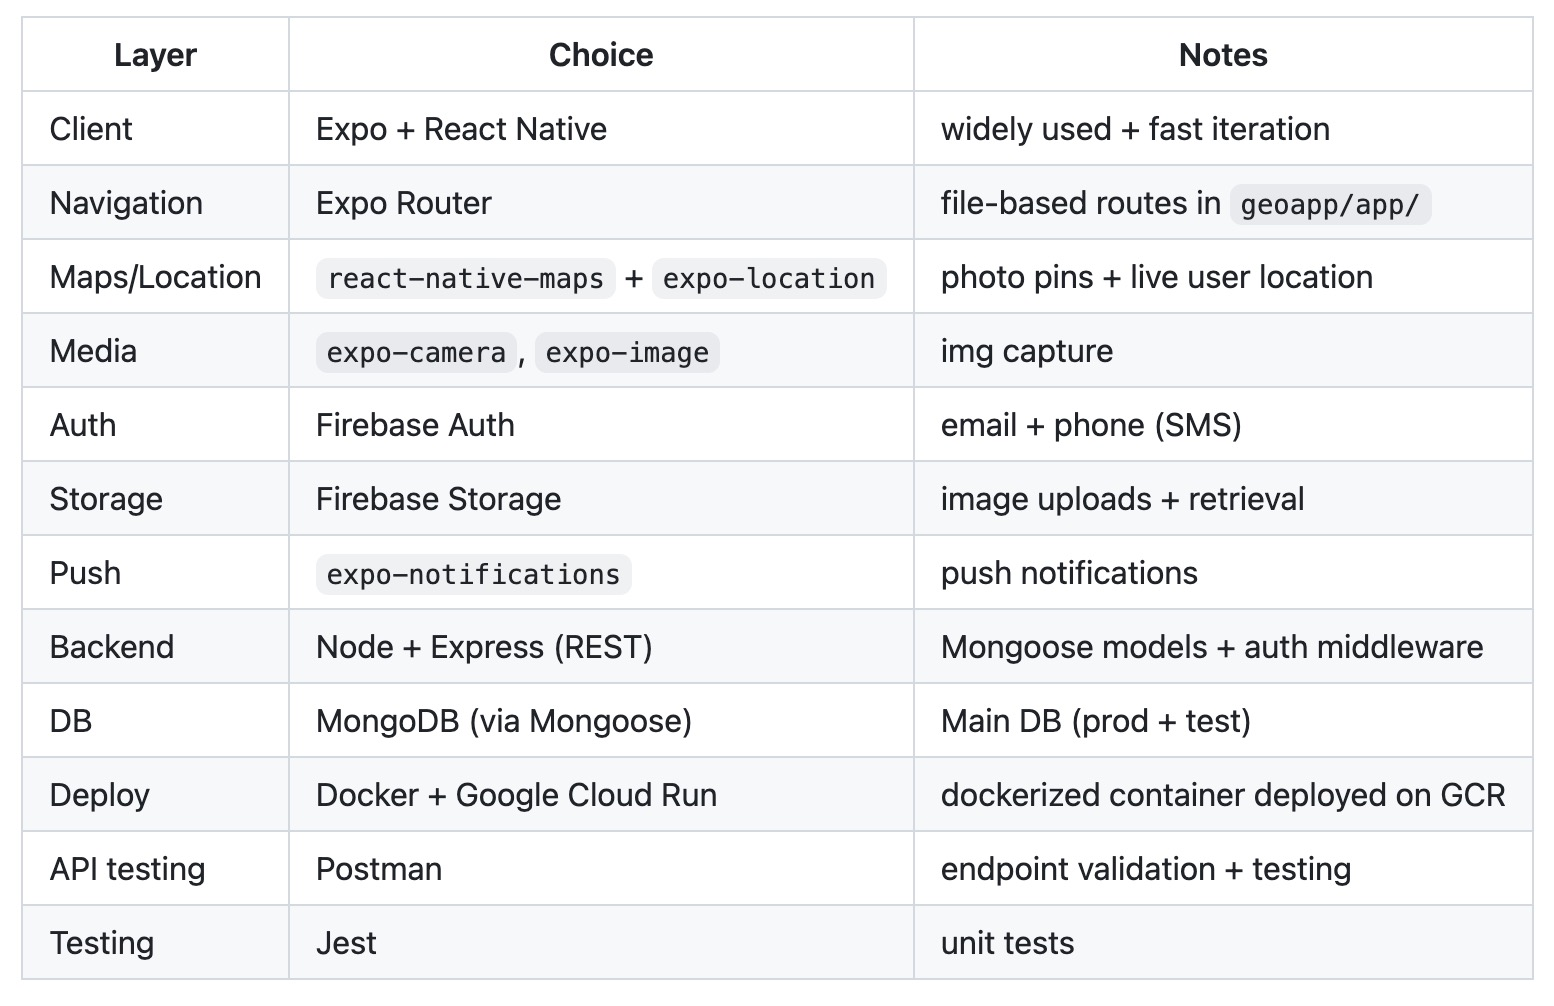
\includegraphics[width=0.7\linewidth]{TechStackChart.jpg}
  \caption{Tech stack overview. \textit{(Core client, backend, and infrastructure components.)}}
  \label{fig:tech-stack}
\end{figure}

\section*{System Architecture and Design Methods}

SideQuest is built as a full-stack system designed for App Store deployment. Each layer of the tech stack was chosen based on trade-offs between iteration speed, scalability, simplicity, and ecosystem familiarity. This section walks through -- and to an extent justifies -- each part of the system: frontend, backend, auth and data, and deployment.


\begin{figure}[!htbp]
  \centering
  
\includegraphics[width=0.95\linewidth]{\detokenize{Latex Created Diagrams/08_navigation_graph.pdf}}
  \caption{Navigation graph diagram.}
  \label{fig:navigation-graph}
\end{figure}


\subsection*{1. Frontend: React Native with Expo}

The client application is built using React Native with the Expo framework. React Native allows the same codebase to compile to both iOS and Android, while still rendering native UI components. This is important for two reasons: while SideQuest is currently iOS-first, it can be deployed to Android without any major rewriting of the app. Second, React Native is widely used across both mobile and web ecosystems (React), meaning familiarity with it is valuable and well-supported by community docs and tooling.

Selecting Expo with React Native is standard practice (once React Native has already been chosen), as it significantly accelearates development. In SideQuest, it provides native support for things like camera access, image handling, push notifications, routing, and location services without any special native configuration. The trade-off is reduced access to certain custom native modules, but for our purposes iteration speed and simplicity greatly outweighs the need for deep native customization. One example of these benefits is the use of \texttt{expo-router}, which provides file-based routing and screen organization. Figure~\ref{fig:navigation-graph} shows the resulting navigation graph, including all frontend screens and the main paths users take between them.

The frontend is compiled and distributed through Apple’s ecosystem using Xcode, App Store Connect, and TestFlight. Many of the most opaque and counterintuitive issues arise from the bloat and strange requirements of this ecosystem. Specifically, we consistently dealt with problems in \texttt{plist} files, build signing, review cycles, the CI/CD pipeline, and general App Store policies. However, the decision to use App Store products is forced on us as a prerequisite to publish on teh App Store, and so the necessary evil it introduces was accepted.

Alternative approaches were considered. A fully native Swift implementation would likely give marginally better performance and deeper integration with Apple APIs, but at the cost of longer development time and no Android compatibility. Flutter was also a viable cross-platform option, but React Native’s JavaScript ecosystem and alignment with the broader MERN stack made React Native the more cohesive choice (same language as backend logic). Though developers may fight against it, as Atwood's law states, ``Any application that can be written in JavaScript, will eventually be written in JavaScript''.


\begin{figure}[!htbp]
  \centering
  
\includegraphics[width=0.95\linewidth]{\detokenize{Latex Created Diagrams/03_sequence_create_challenge.pdf}}
  \caption{Sequence diagram: create challenge flow.}
  \label{fig:sequence-create-challenge}
\end{figure}

\begin{figure}[!tb]
  \centering
  
\includegraphics[width=0.7\linewidth]{\detokenize{Latex Created Diagrams/04_sequence_global_duel_vote_token.pdf}}
  \caption{Sequence diagram: Duel vote token flow.}
  \label{fig:sequence-global-duel-vote-token}
\end{figure}


\subsection*{2. Backend: Node.js with Express (MERN)}
The backend is built using Node.js and Express, forming part of the MERN (MongoDB, Express, React, Node) stack. Node.js allows JavaScript to run server-side. Using the same language across frontend and backend reduces context switching and improves development speed. Express is a REST API layer that is simple, flexible, and widely adopted. The primary advantage of this stack is cohesion. React on the frontend and Node/Express on the backend share conceptual patterns (components, middleware, JSON APIs). This makes it easy to reason about how data flows across the system.

Alternative backend frameworks were considered. Python (Flask or Django) would provide strong tooling and readability. Additionally, I have significant prior experience with both Python and Flask, and thus would initially have been much more comfortable with this backend. However, the flexibility and ecosystem alignment of Express made it better suited for rapid iteration and a custom-designed API. A more rigid framework would increase complexity, something against our design philosophy.

For an overall sense of the way in which frontend and backend interact, figures~\ref{fig:sequence-create-challenge} and~\ref{fig:sequence-global-duel-vote-token} illustrate examples of client–server interactions. Figure~\ref{fig:sequence-create-challenge} traces the create new challenge flow, wherein user input is sent in a POST API request. The backend then validates, writes to DB, and returns a response, allowing the newly created pin to be displayed to all users. Figure~\ref{fig:sequence-global-duel-vote-token} shows the slightly more complicated 'voting' token flow, during which the user receives a pair of photos to vote on, validated by a minted TTL token from the backend. The vote pair and token minting are fetched on app start using GET \texttt{global\_duel}, randomizing an 'Elo' bucket combination to return from (preferring better photos) and returning a photo pair. Voting then occurs using POST \texttt{vote\_duel\_global}, with the backend consuming the token and persisting to the DB. Invalid tokens are used to enforce hourly voting limits and ensure users are properly authenticated. In addition to error handling, this helps prevent problems similar to that which faced DKUMash: botting of votes will quickly be caught and invalidated.

Broadly, the takeaway is that the backend enforces server-authoritative logic. All ranking updates, vote validation, and rate limiting occur server-side. This prevents manipulation from the client and preserves integrity.

\begin{figure}[!htbp]
  \centering
  
\includegraphics[width=0.95\linewidth]{\detokenize{Latex Created Diagrams/01_domain_data_model.pdf}}
  \caption{Domain data model diagram.}
  \label{fig:domain-data-model}
\end{figure}


\subsection*{3. Data Architecture and Authentication}

\subsubsection*{3.1 Database: MongoDB Atlas + Mongoose}

SideQuest uses MongoDB Atlas as its primary database. MongoDB is a document-oriented database, meaning it stores JSON-like documents rather than strictly relational tables. This allows for flexible schema evolution, which was valuable during early development when data models changed frequently.

MongoDB was selected partially due to its generous free tier and ease of cloud deployment. Atlas provides managed hosting, backups, and scaling without requiring infrastructure management.

However, MongoDB is not relational in the traditional SQL sense. To introduce structure and validation, Mongoose is used as an Object Data Modeling (ODM) layer. Mongoose defines schemas, enforces validation rules, and creates relationships between collections. While MongoDB itself does not enforce foreign key constraints, Mongoose allows us to simulate relational structure through references and schema design.

A relational SQL database (ex: PostgreSQL) was considered. SQL databases provide stronger built-in relational guarantees and transactional consistency. However, SideQuest data shape is naturally hierarchical and document shaped, not deeply relational. For example, a given pin is usually fetched as a nested JSON in the API response regardless: thus, the symmetry feels both natural and convenient. Additionally, MongoDB has a faster iteration model, and lets us evolve documents without migrations. With Postgress, schema migrations would be required each time we changed data models, which has been troublesome on past projects. With MongoDB, after migration old data can simply be missing from the schema without causing errors, and can be backfilled either with a script or handled through well chosen defaults. For a rapidly changing product, schema rigidity can slow development.

Mongoose defines the MongoDB schema, introducing relational-style structure to the DB (much to the delight of Professor Mustafa Misir). Figure~\ref{fig:domain-data-model} summarizes the core collections and how they reference one another, including user identies, challenges/pins, and interaction records such as votes. Notice how user ID (uid) and pin ID are used as the primary key for most collections. Most relationships are keyed as 1: many (except when normalizing tables, generally keyed in 1:1 relationships). These relationships are important for keeping server-side logic consistent and minimizing DB writes when possible.

\subsubsection*{3.2 Media Storage: Firebase Storage}

Images are not stored directly in MongoDB. Instead, image files are uploaded to Firebase Storage, and only their URIs are stored in the database.

Storing images directly inside MongoDB (for example, as binary blobs) would dramatically increase database size and degrade performance. Databases are optimized for structured data, not large media objects. Separating media storage from structured data is standard practice in production systems. Firebase Storage provides scalable object storage optimized for large files. This separation keeps the database efficient and independent.

\subsubsection*{3.3 Authentication: Firebase Auth}

Authentication is handled using Firebase Authentication. Users can sign in via phone (SMS), email, or Google account.

Implementing authentication from scratch would require handling password hashing, token management, SMS verification infrastructure, and security auditing. Firebase abstracts this complexity while still allowing server-side token verification using Firebase Admin SDK.

All privileged backend routes verify Firebase-issued ID tokens before allowing writes. This ensures that authentication is also enforced server-side, securing server routes.

\subsection*{4. Deployment, Containerization, and Testing}

The backend is containerized using Docker.  A common developer joke captures the problem Docker is meant to solve: a developer's code works locally, but upon pushing to someone else's production it immediately breaks. The developer simply shrugs and responds, "It works on my machine", washing his hands of the issue. This is frequently distressing to those impacted by the issue. Docker is intended to eliminate this problem, by standardizing the execution environment. Containerization ensures the application runs identically across development and production environments. Dependencies, Node versions, and environment variables are packaged consistently.

In production, the Docker container is deployed to Google Cloud Run. Cloud Run automatically scales instances based on traffic and provides global accessibility without managing servers manually. Compared to traditional VM hosting, Cloud Run abstracts infrastructure management while still allowing full control over the runtime environment.

Alternative deployment options include Heroku or traditional virtual machines. However, Docker + Cloud Run provided greater control and scalability without excessive complexity. Additionally, the CI/CD pipeline was incredibly easy to set up, and the service is generally very straightforward to work with.

For API validation and debugging, Postman is used to test endpoints independently of the frontend. This allows for isolating backend issues without UI interference. Jest is used for unit testing critical backend logic.

\subsection*{5. User Testing and Iterative Validation}

\begin{wrapfigure}[9]{r}{0.4\linewidth}
  \vspace{-2\baselineskip}
  \centering
  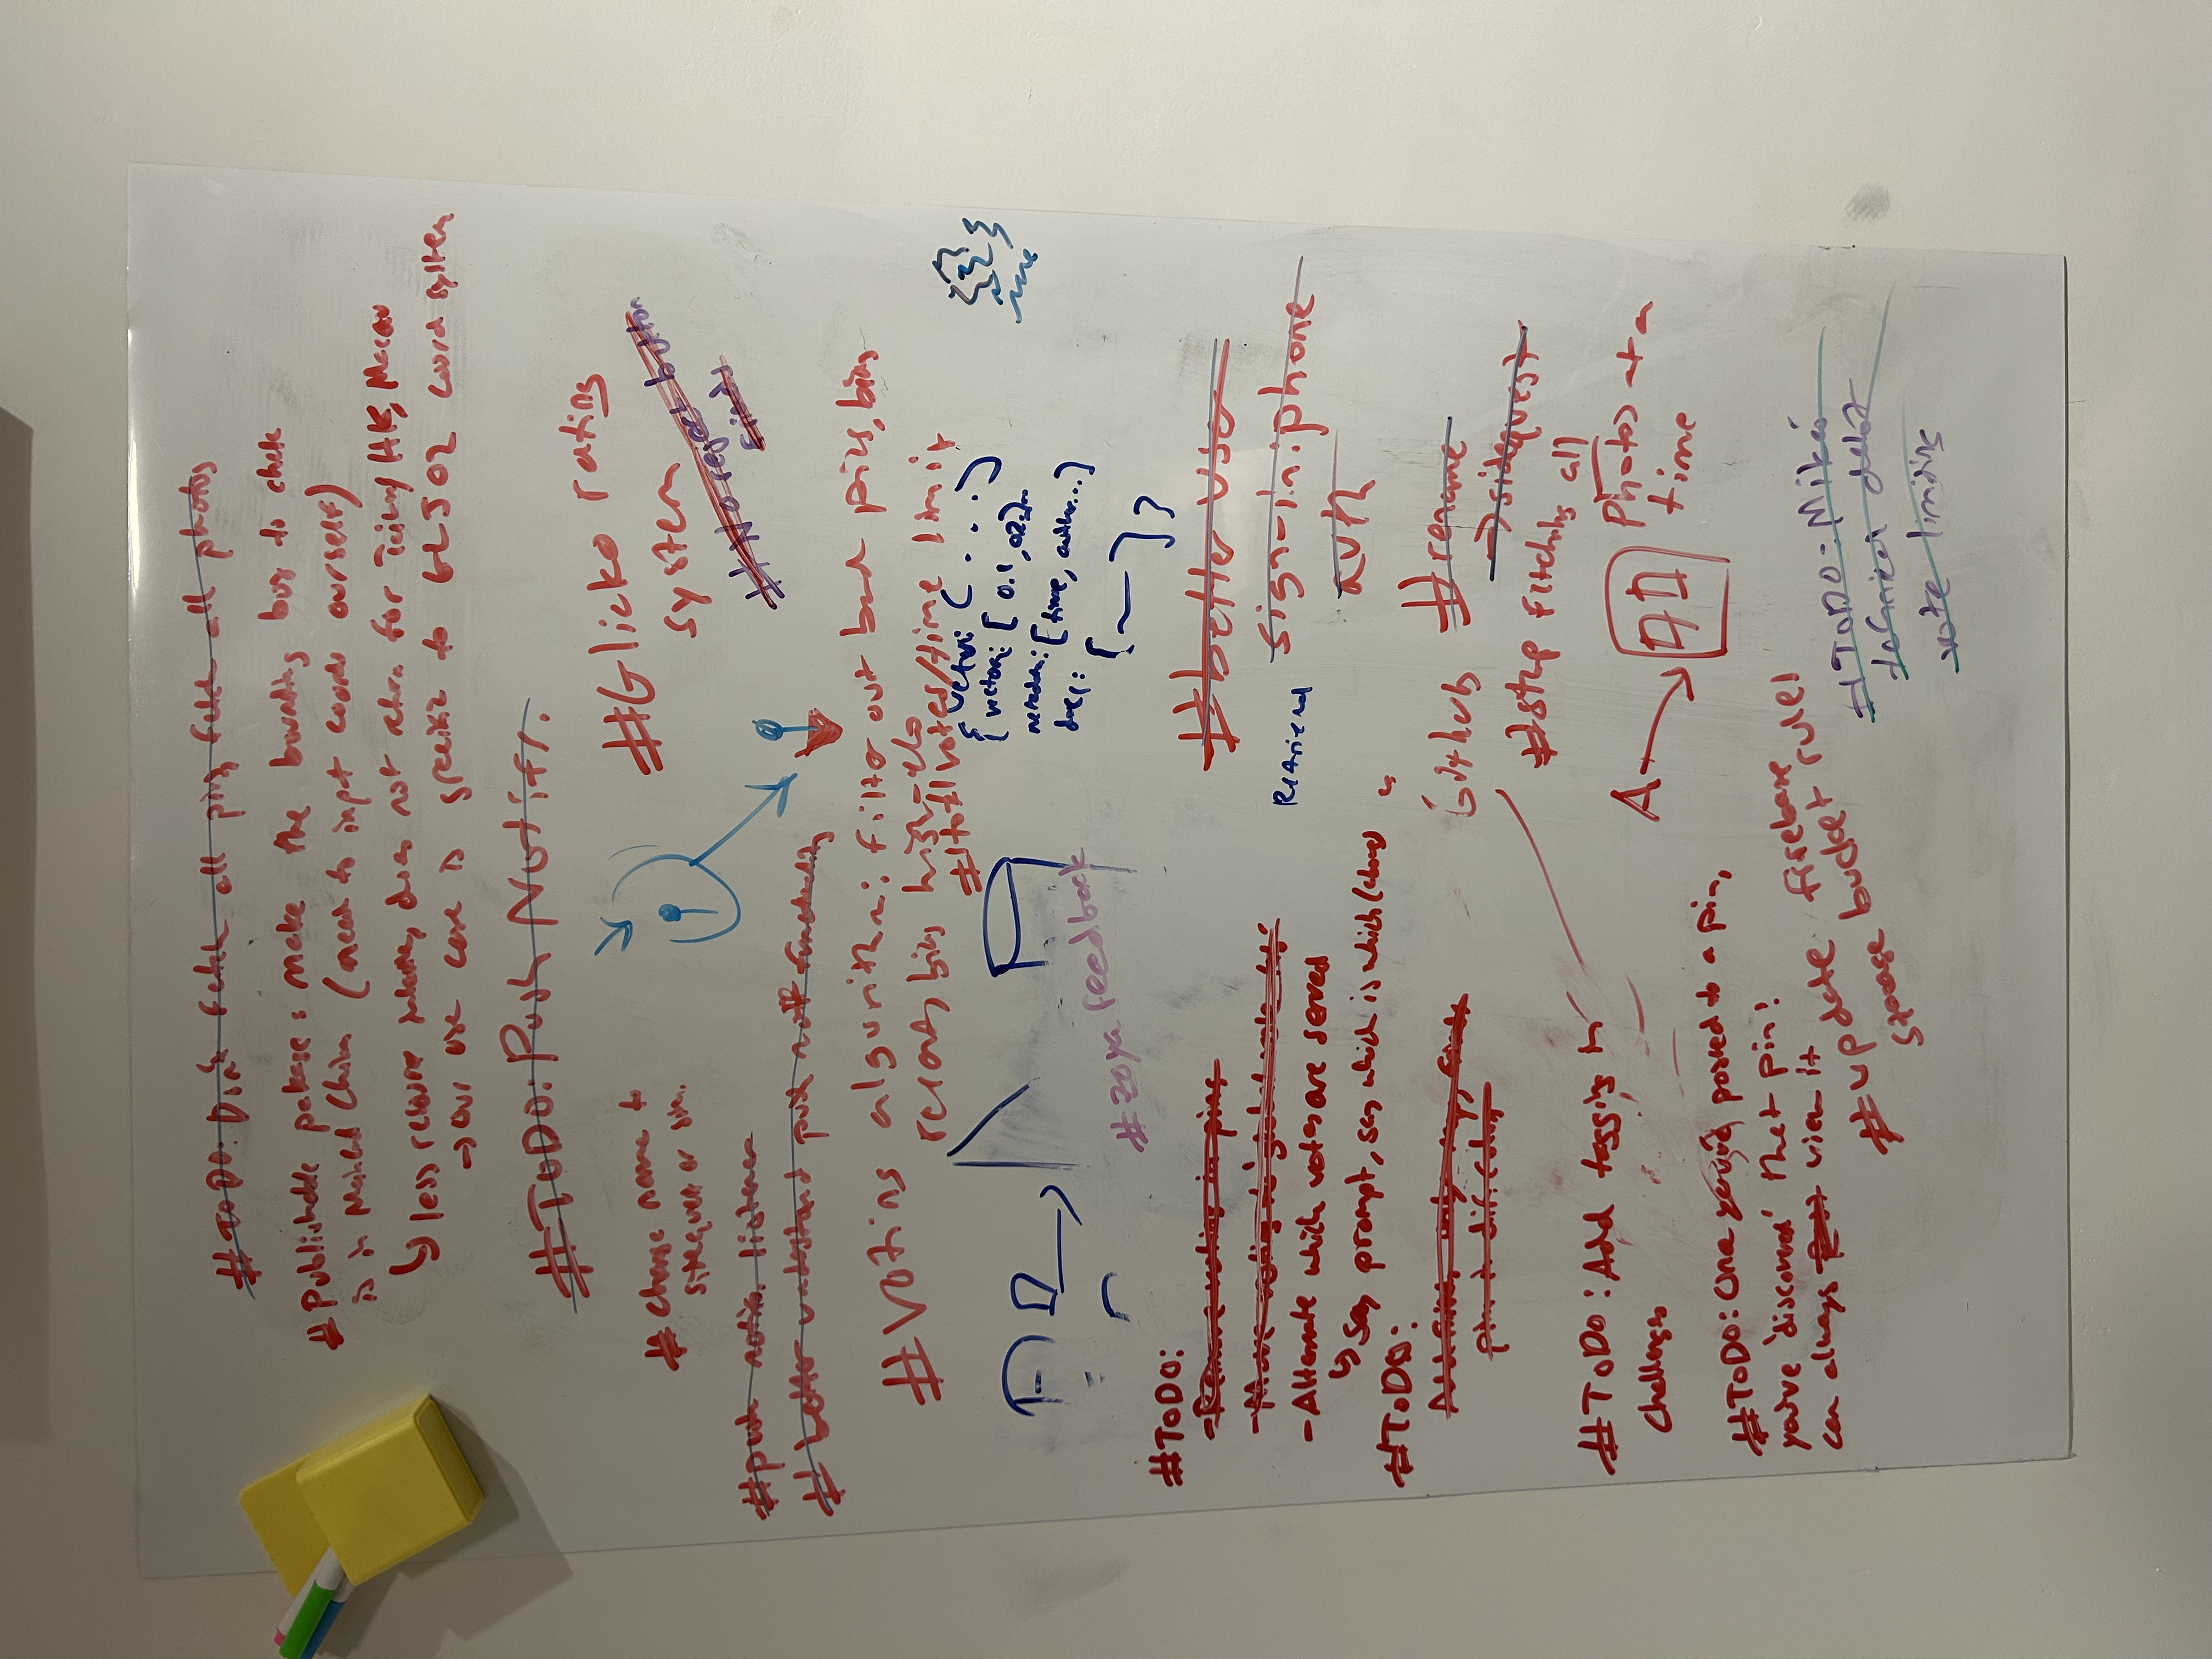
\includegraphics[width=\linewidth, angle=-90]{UserFeedbackWall.jpeg}
  \caption{Whiteboard backlog used to track open issues.}
  \label{fig:user-feedback-wall}
\end{wrapfigure}

SideQuest’s architecture decisions are heavily driven by user feedback and TestFlight deployment.

\subsubsection*{5.1 TestFlight as Formal Evaluation Channel}

TestFlight builds were released in rapid cycles. Each release included observed task flows, post-session qualitative feedback, and bug reproduction. This method allows for controlled evaluation of user UX smoothness, upload reliability, and issue detection.

\subsubsection*{5.2 Selected User Feedback and Responses}

The documented user feedback revealed abundant major issue categories. We noted qualitative feedback both on a 'product backlog' whiteboard \textit{(Fig.~\ref{fig:user-feedback-wall})}, as well as in a shared Obsidian notes app. A small selection of user problems and resolutions are included in the below table (Fig.~\ref{fig:user-feedback-table})


\begin{figure}[!b]
  \centering
  \renewcommand{\arraystretch}{1.25}
  \begin{tabular}{|p{0.32\linewidth}|p{0.62\linewidth}|}
  \hline
  \textbf{Identified problem} & \textbf{Resolution} \\
  \hline
  Swipe voting: flicker during swipes. & Image prefetch introduced; optimistic UI updates \\
  \hline
  Upload reliability issues: unclear upload state. & Promise resolution tracking; UI toast (notification message) on success \\
  \hline
  Aesthetic issues: poor cohesiveness. & Unified palette implementation; shared component primitives. \\
  \hline
  Elo integrity: ranking manipulation. & Token-based duel confirmation; rate limits and hourly caps. \\
  \hline
  \end{tabular}
  \caption{Selected user feedback issues and implemented resolutions.}
  \label{fig:user-feedback-table}
\end{figure}

\subsection*{6. Design Methods }

As we have already talked extensively about theory, this section aims to discuss specific process innovations and implementation.

\subsubsection*{3.1 Production Prototyping}

Instead of designing visuals first and engineering later, SideQuest follows a 'capability-first' method. Roughly, this means that system functionality is built out first (backend), and UI is designed around system constraints. This allows for simple UI iteration with confidence and catching concurrency bugs early.

\subsubsection*{3.2 Agile Development }

Development prioritized constant iterative improvement based on user feedback, following the Agile development philosophy. Each cycle began with a TestFlight release, followed by direct observation of user interaction (Fig. ~\ref{fig:agile-cycle}).

As issues emerged, we revisited architectural components in real time. It is important to have little emotional attachment to the current state of the project, and readily refactor when necessary. In several cases, this resulted in major overhauls of the app. After implementing changes, a new build was released and the cycle repeated. Over time, this iterative pattern functions like gradient descent optimization, as iterative releases gradually move the user toward a smoother product experience.

This process assumes that all of our assumptions are incorrect. Design and architecture remains highly fluid.

\subsubsection*{3.3 Git-Based Dev }

Git is simply incredible, and deserves an honorable mention. Git was used for version control and structured iteration.

Minimal-diff commits were important for identifying isolated behavior changes. One example of this is when fixing a particularly nasty UI bug related to issues only on every 3rd served photo, it was necessary to revert commits back several weeks to localize when the problem originated. Only by reverting to an earlier version was the problem identified and solved. Commit history also serves as a repository of product evolution and architectural maturation \textit{(Fig.~\ref{fig:repo-commit-diagram})}.

\begin{figure}[!htbp]
  \centering
  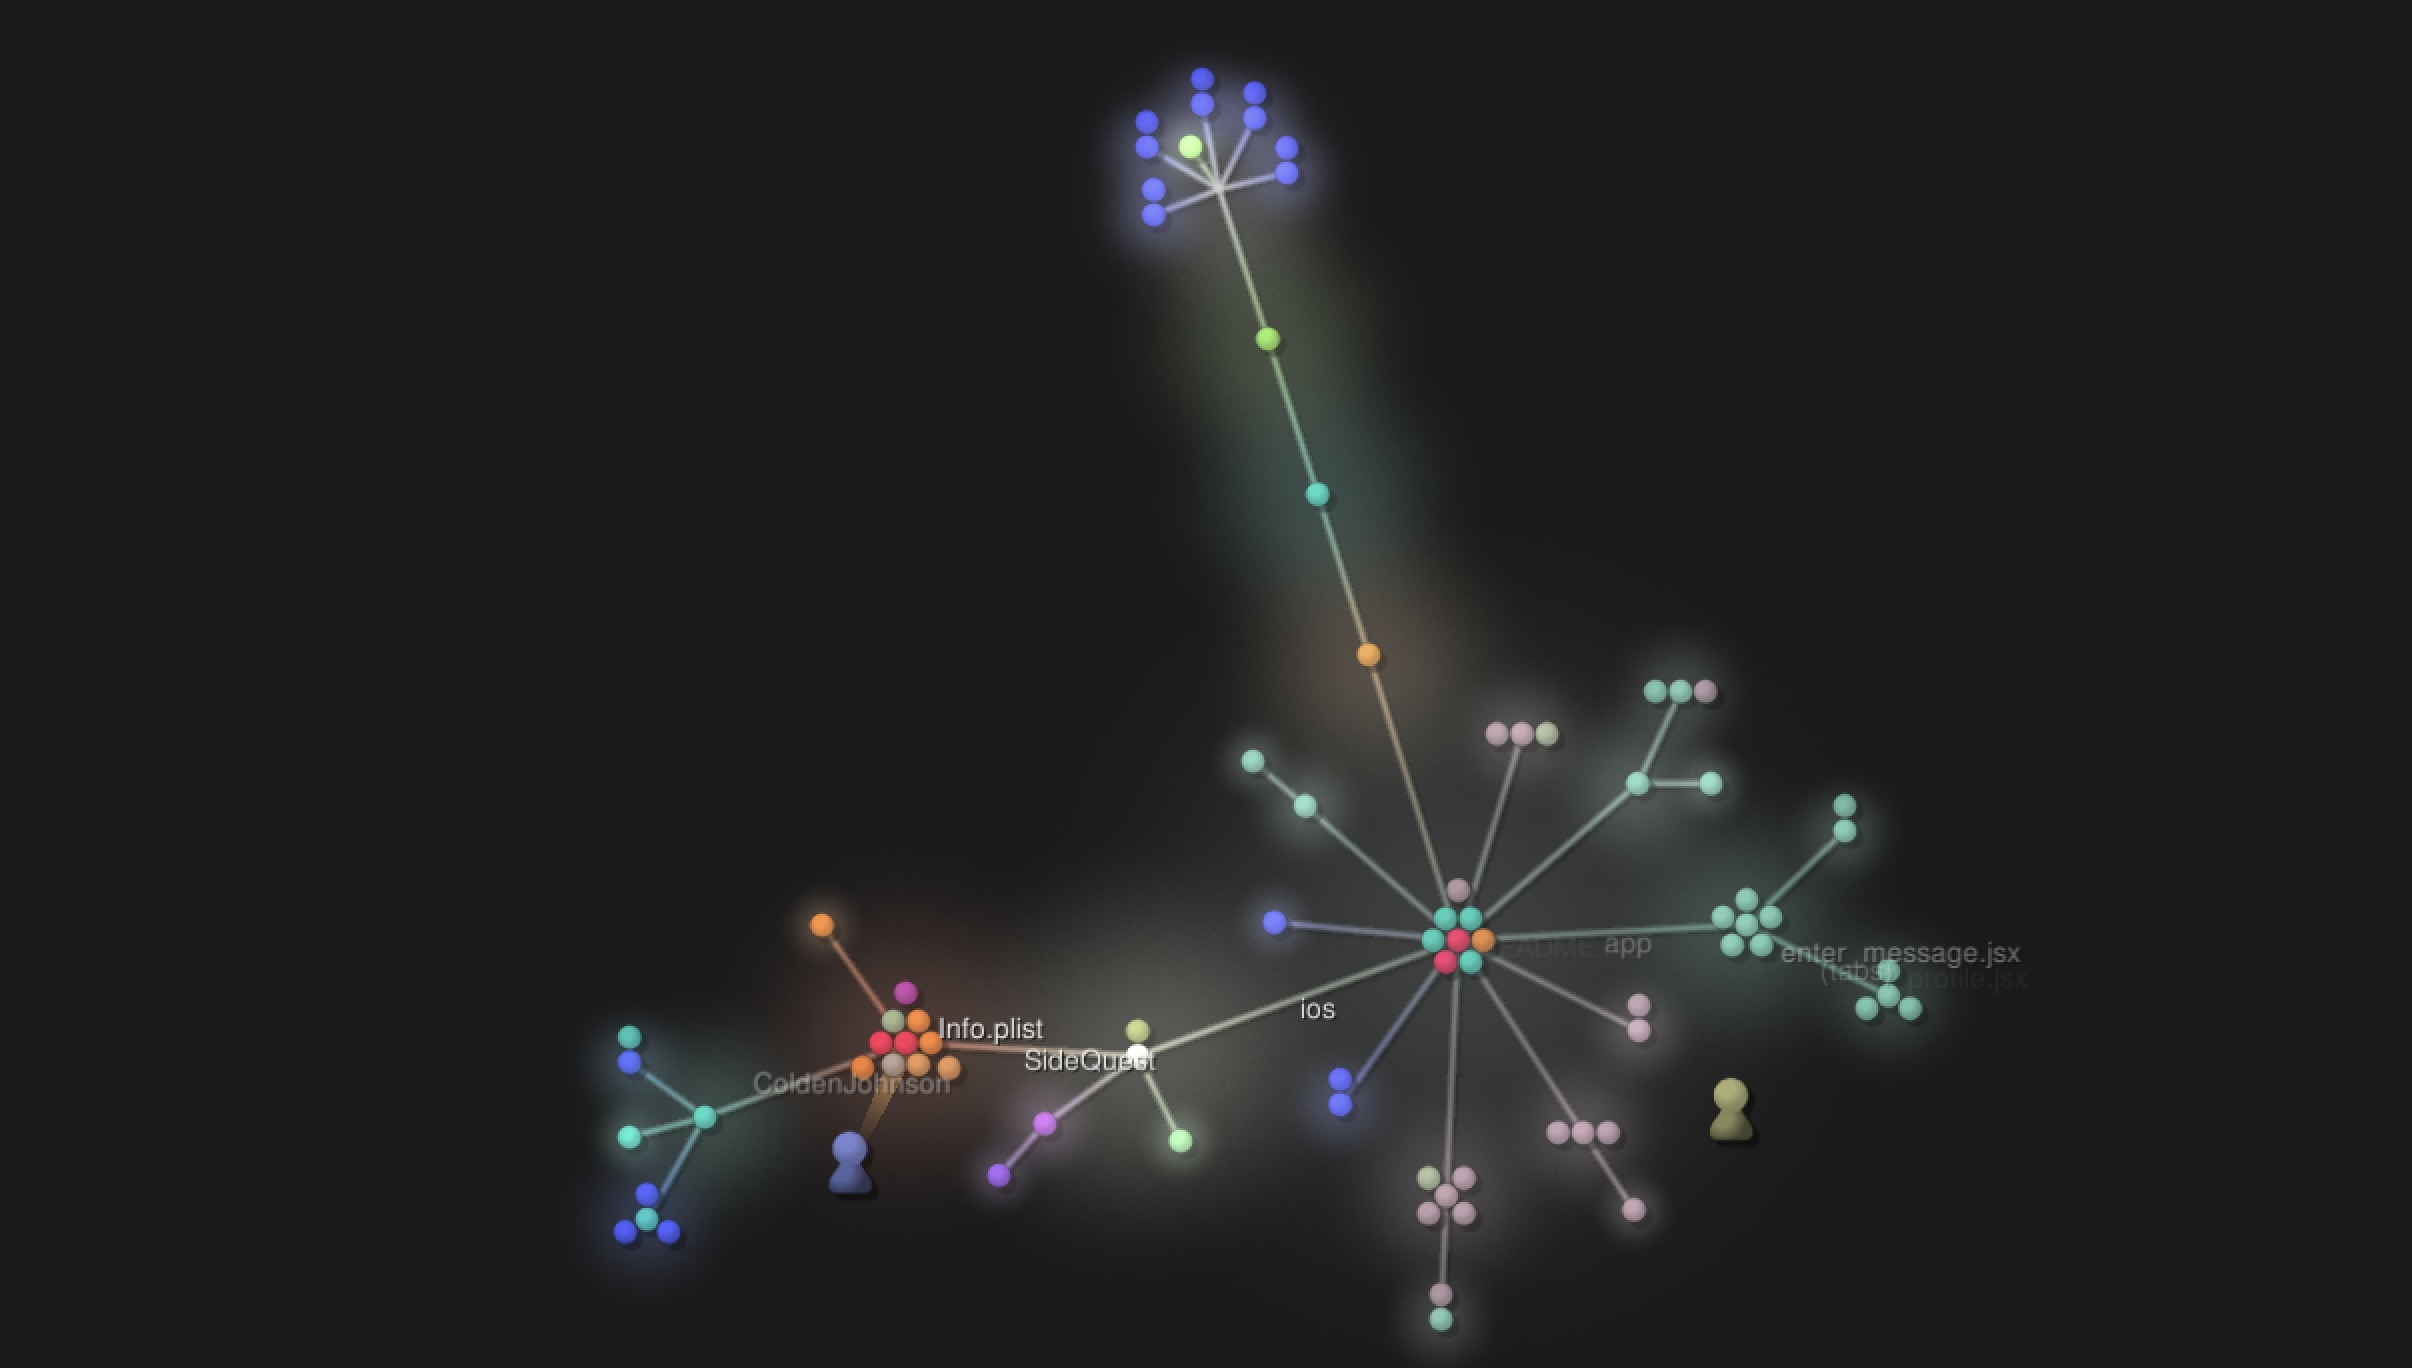
\includegraphics[width=0.9\linewidth]{RepoCommitDiagram.jpg}
  \caption{Gource Git commit visualization with multiple contributors and versioning.}
  \label{fig:repo-commit-diagram}
\end{figure}

\subsection*{7. AI Usage In Modern Development }

AI usage in modern app development is an entire paper on its own. That said, it is instructive to talk briefly about the ways we're using AI in our workflows and how it assists with architectural judgement.

We use primarily Codex 5.3 for simple implementation-related coding tasks. Architectural decisions are typically informed using a mix of Claude and ChatGPT (along with docs/example GitHubs). This separation is relatively strict, as models perform best when given well-scoped problems. In our workflow, we have found that spending the majority of time upfront thinking about architecture results in far easier implementation later on.

We maintain an extensive custom prompt and model library for recurring tasks. For example, our `summary' task is adapted from a leaked Claude Code summary template, and is used to prevent context overload during extended terminal sessions. Context management more broadly is critical. To address this, we use a combination of MCP servers for scoped context exposure, deep research for highly complex decisions, and manual identification of relevant documentation and code snippets when pursuing specific directions. In addition, we run several custom model configurations within a local Open WebUI instance connected to OpenRouter \textit{(see Fig.~\ref{fig:openwebui-example})}. These custom models allow for targeting specific jobs/recurring problem categories (for example, dealing with Elo/ranking logic or writing README documentation).

In short, AI is an important aspect of modern development, and we have put a significant amount of energy into setting up appropriate workflows to fully take advantage of this.

\begin{figure}[!htbp]
  \centering
  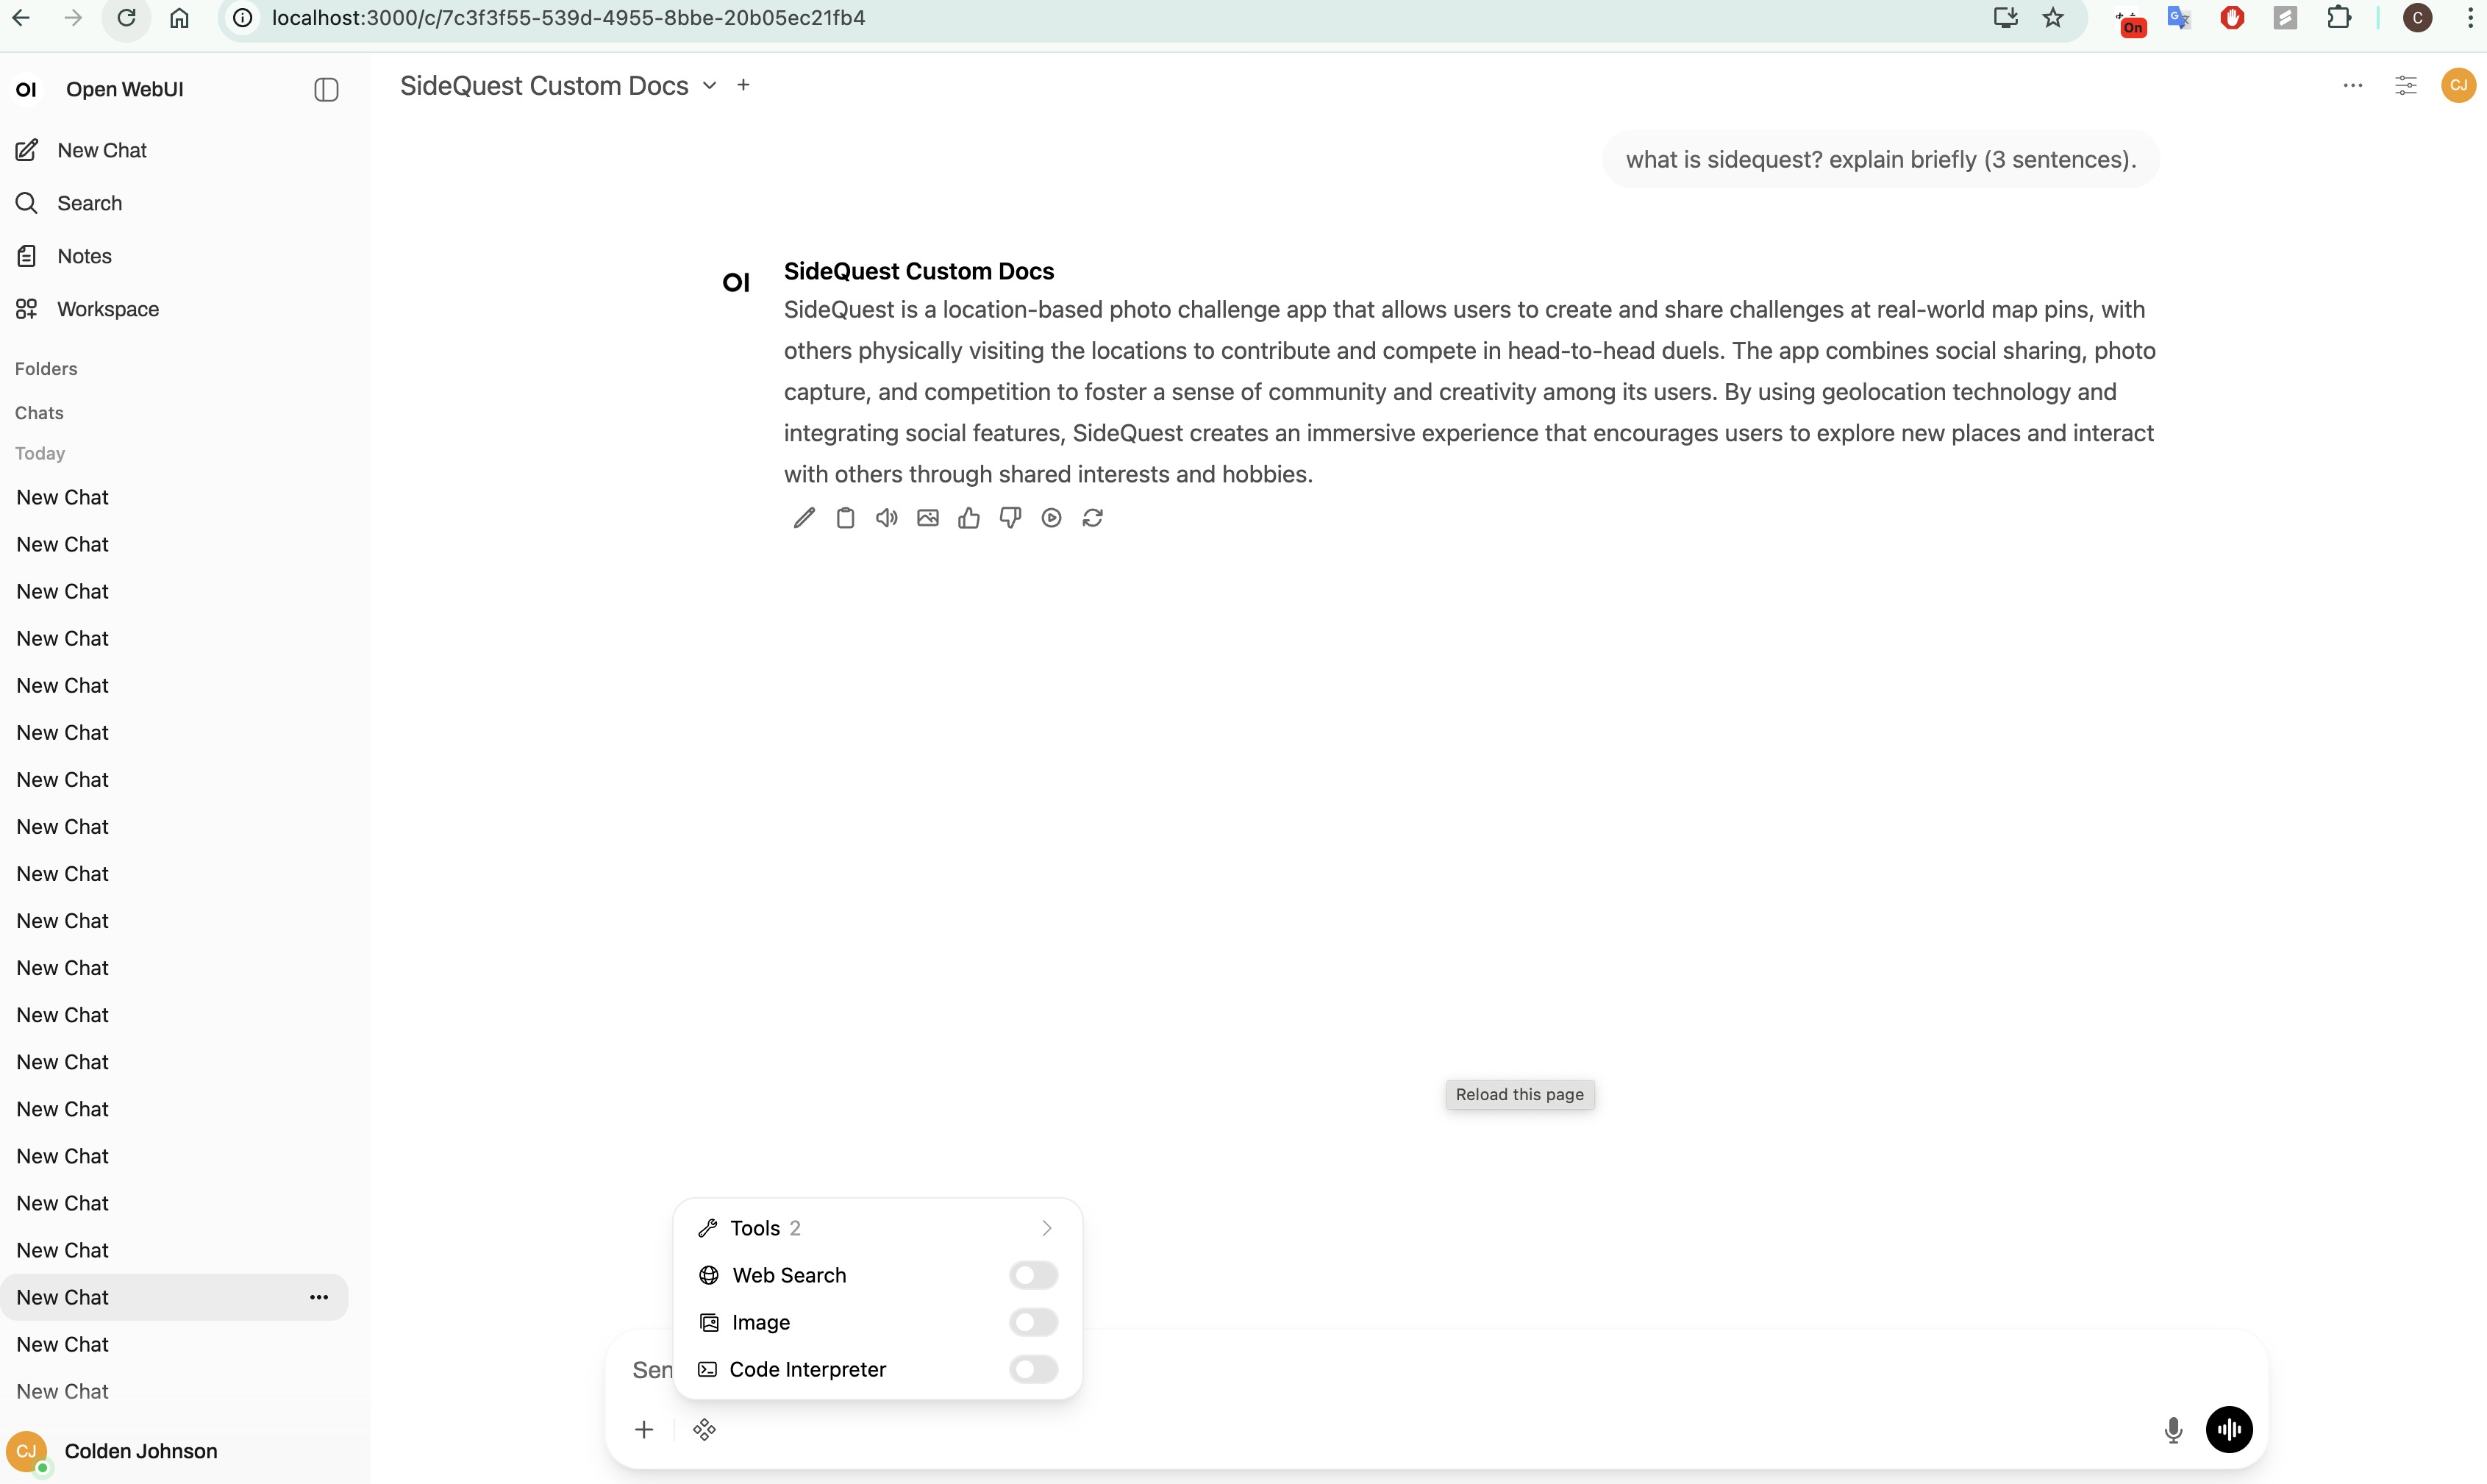
\includegraphics[width=0.5\linewidth]{OpenWebUI_example.jpg}
  \caption{Open WebUI local model workflow. \textit{Example of custom model config used for scoped, recurring docs querying/generation.}}
  \label{fig:openwebui-example}
\end{figure}

% =========================
% FINAL OUTCOME
% =========================
\section*{FINAL OUTCOME}
\subsection*{5.1 Concept statement}
SideQuest is a creative platform that transforms spaces into living, community-built creative artifacts. A user stands somewhere, captures a moment, adds a short prompt, and plants that creative challenge onto a map. Over time, this space becomes a shared public square shaped by many contributors. 

SideQuest is 'the anti-Instagram': while many social platforms reward passive scrolling, SideQuest asks users to explore and create.

Beyond being an innovative concept, SideQuest is a successful example of a full-stack iOS application published to the App Store and supported by production-grade architecture. The system manages authentication, media storage, geospatial correctness, and user interaction. It has X daily active users, providing evidence that the design holds under real usage conditions.

\subsection*{5.2 What is delivered (artifact inventory)}
This project delivers a complete set of artifacts suitable for a creative practice Signature Work:

\textbf{Primary artifact}
\begin{itemize}[leftmargin=*, itemsep=0.25\baselineskip]
  \item SideQuest iOS App
\end{itemize}

\textbf{Supporting artifacts}
\begin{itemize}[leftmargin=*, itemsep=0.25\baselineskip]
  \item Deployed backend (Dockerized API on Google Cloud Run)
  \item GitHub repository (source code, history, documentation)
  \item Design + testing documentation (TestFlight feedback notes; iterative change history)
  \item Evaluation evidence (DAU trend snapshots; usability findings; bug/issue log excerpts)
  \item Screenshots and visual documentation (final UI states for major flows)
  \item Architecture diagrams
\end{itemize}

\subsection*{5.4 Walkthrough of the final user experience}
<TODO: Upload screenshots here>
Let's look at our friend Krishna's user journey:


-onboarding + SMS
- live map screen
- challenge creation and contribution
-voting, viewing, immersion
-competition and motivation (gamification, duels)
-adding friends

\subsection*{5.5 Evidence of impact}
<TODO:  DAUs, Example challenge pin, outcome metrics table>

<TODO: Reflection, Bibliography, Prof. Feedback>

\begin{figure}[!htbp]
  \centering
  \begin{minipage}[t]{0.48\linewidth}
    \centering
    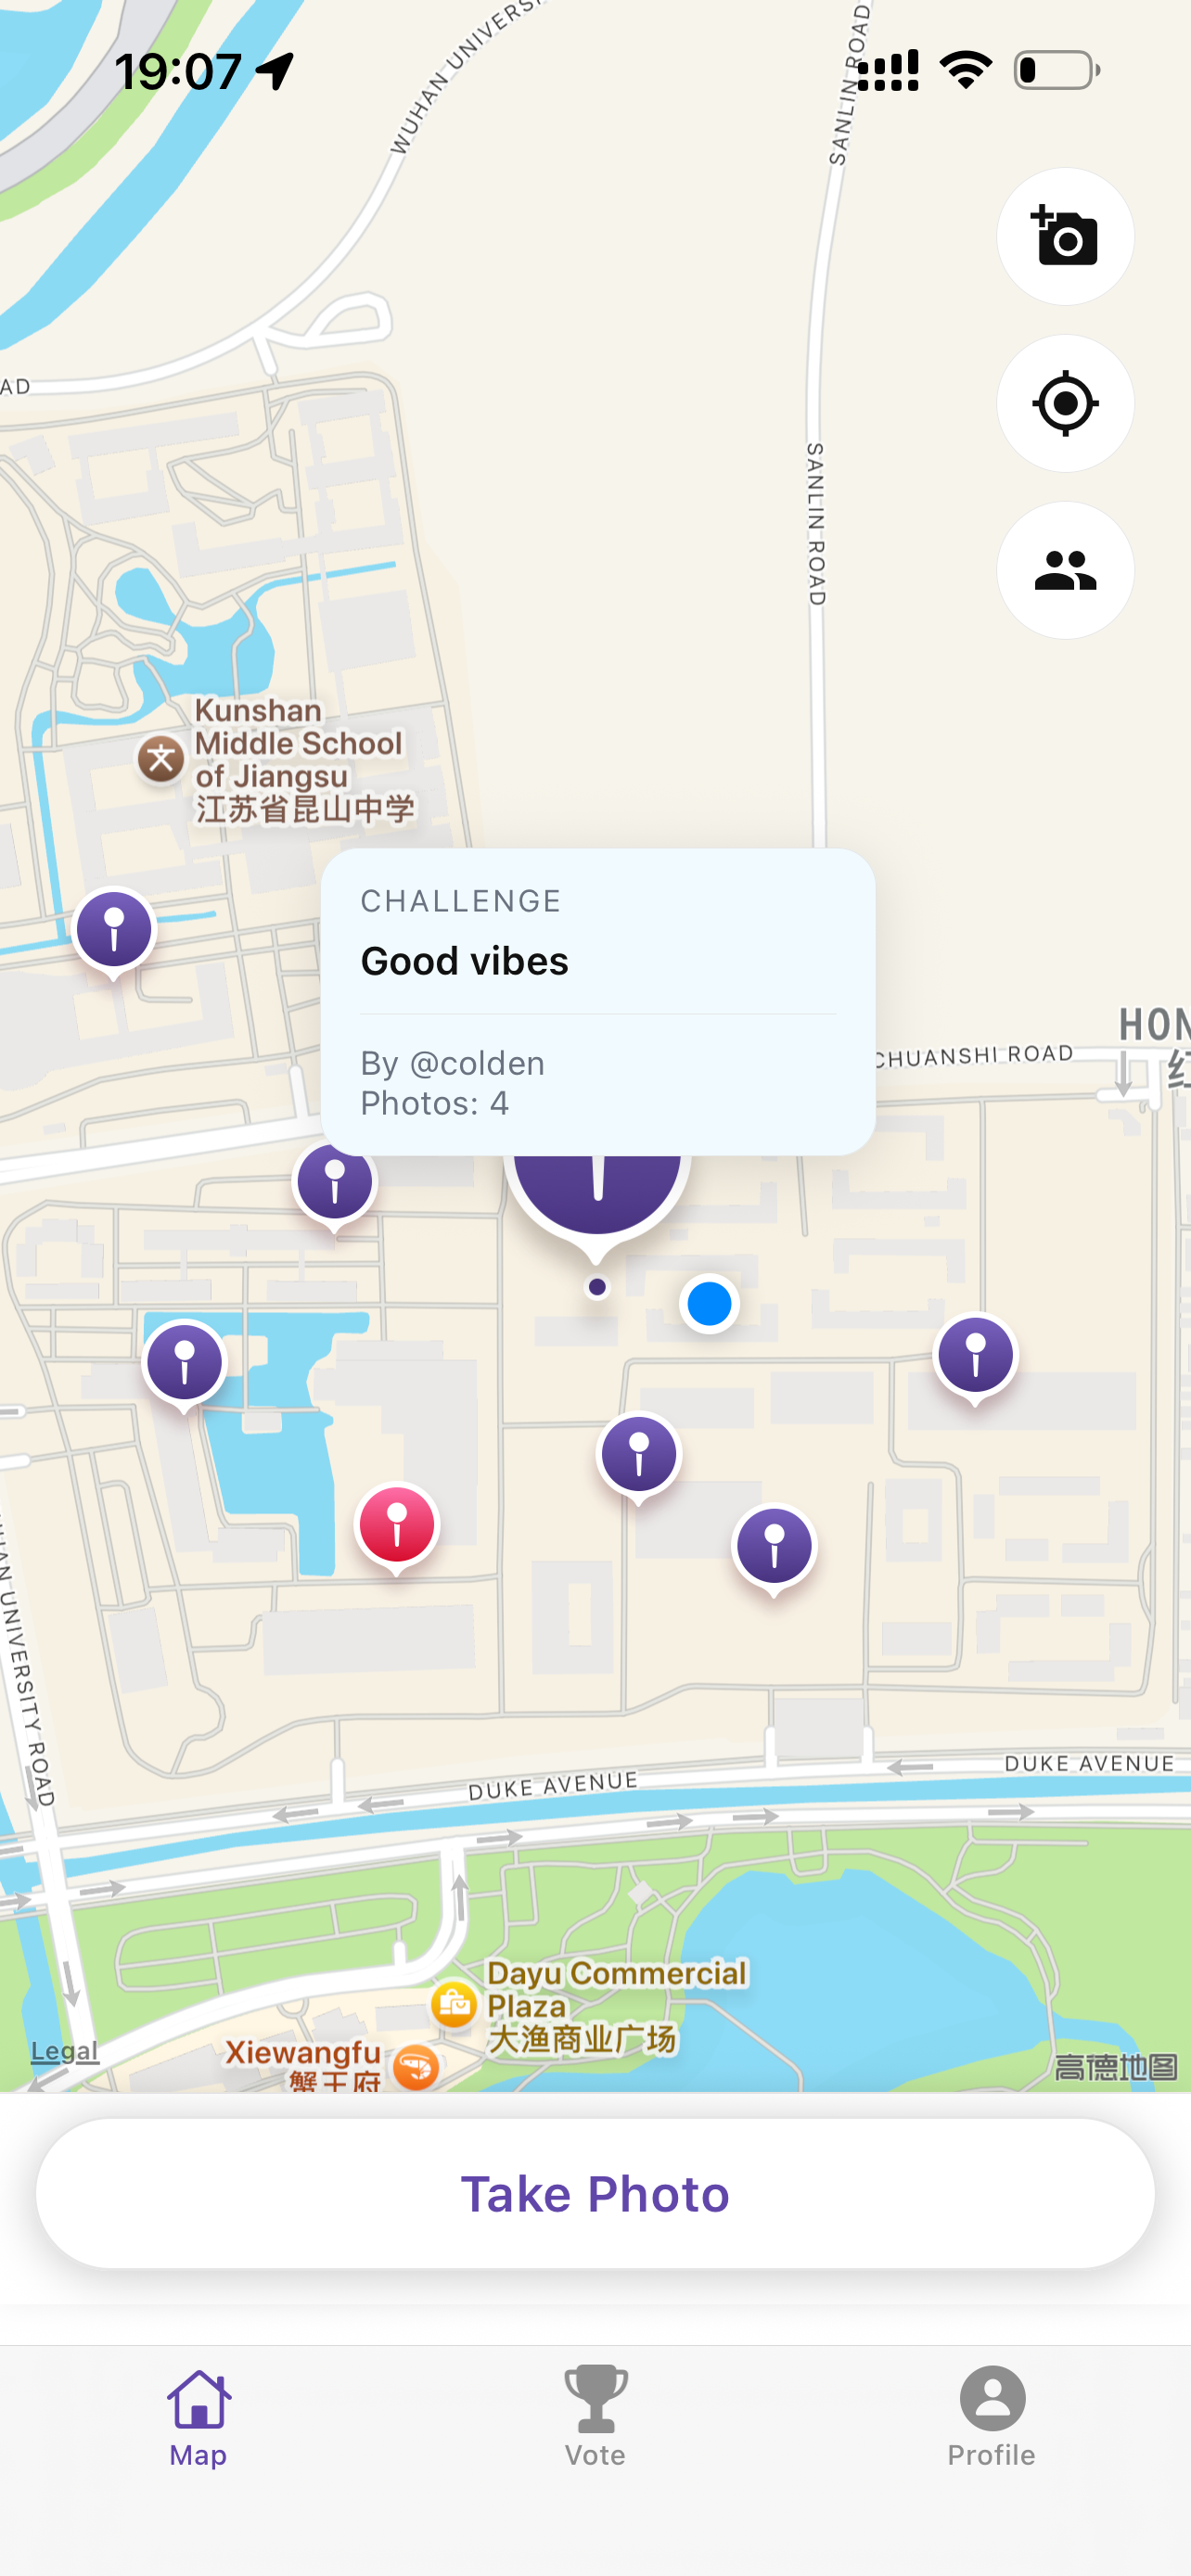
\includegraphics[width=\linewidth]{ChallengeMap.PNG}
    \caption{Challenge map landing page. \textit{(Landing page map view with pin uploads around DKU created by app users.)}}
    \label{fig:challenge-map}
  \end{minipage}\hfill
  \begin{minipage}[t]{0.48\linewidth}
    \centering
    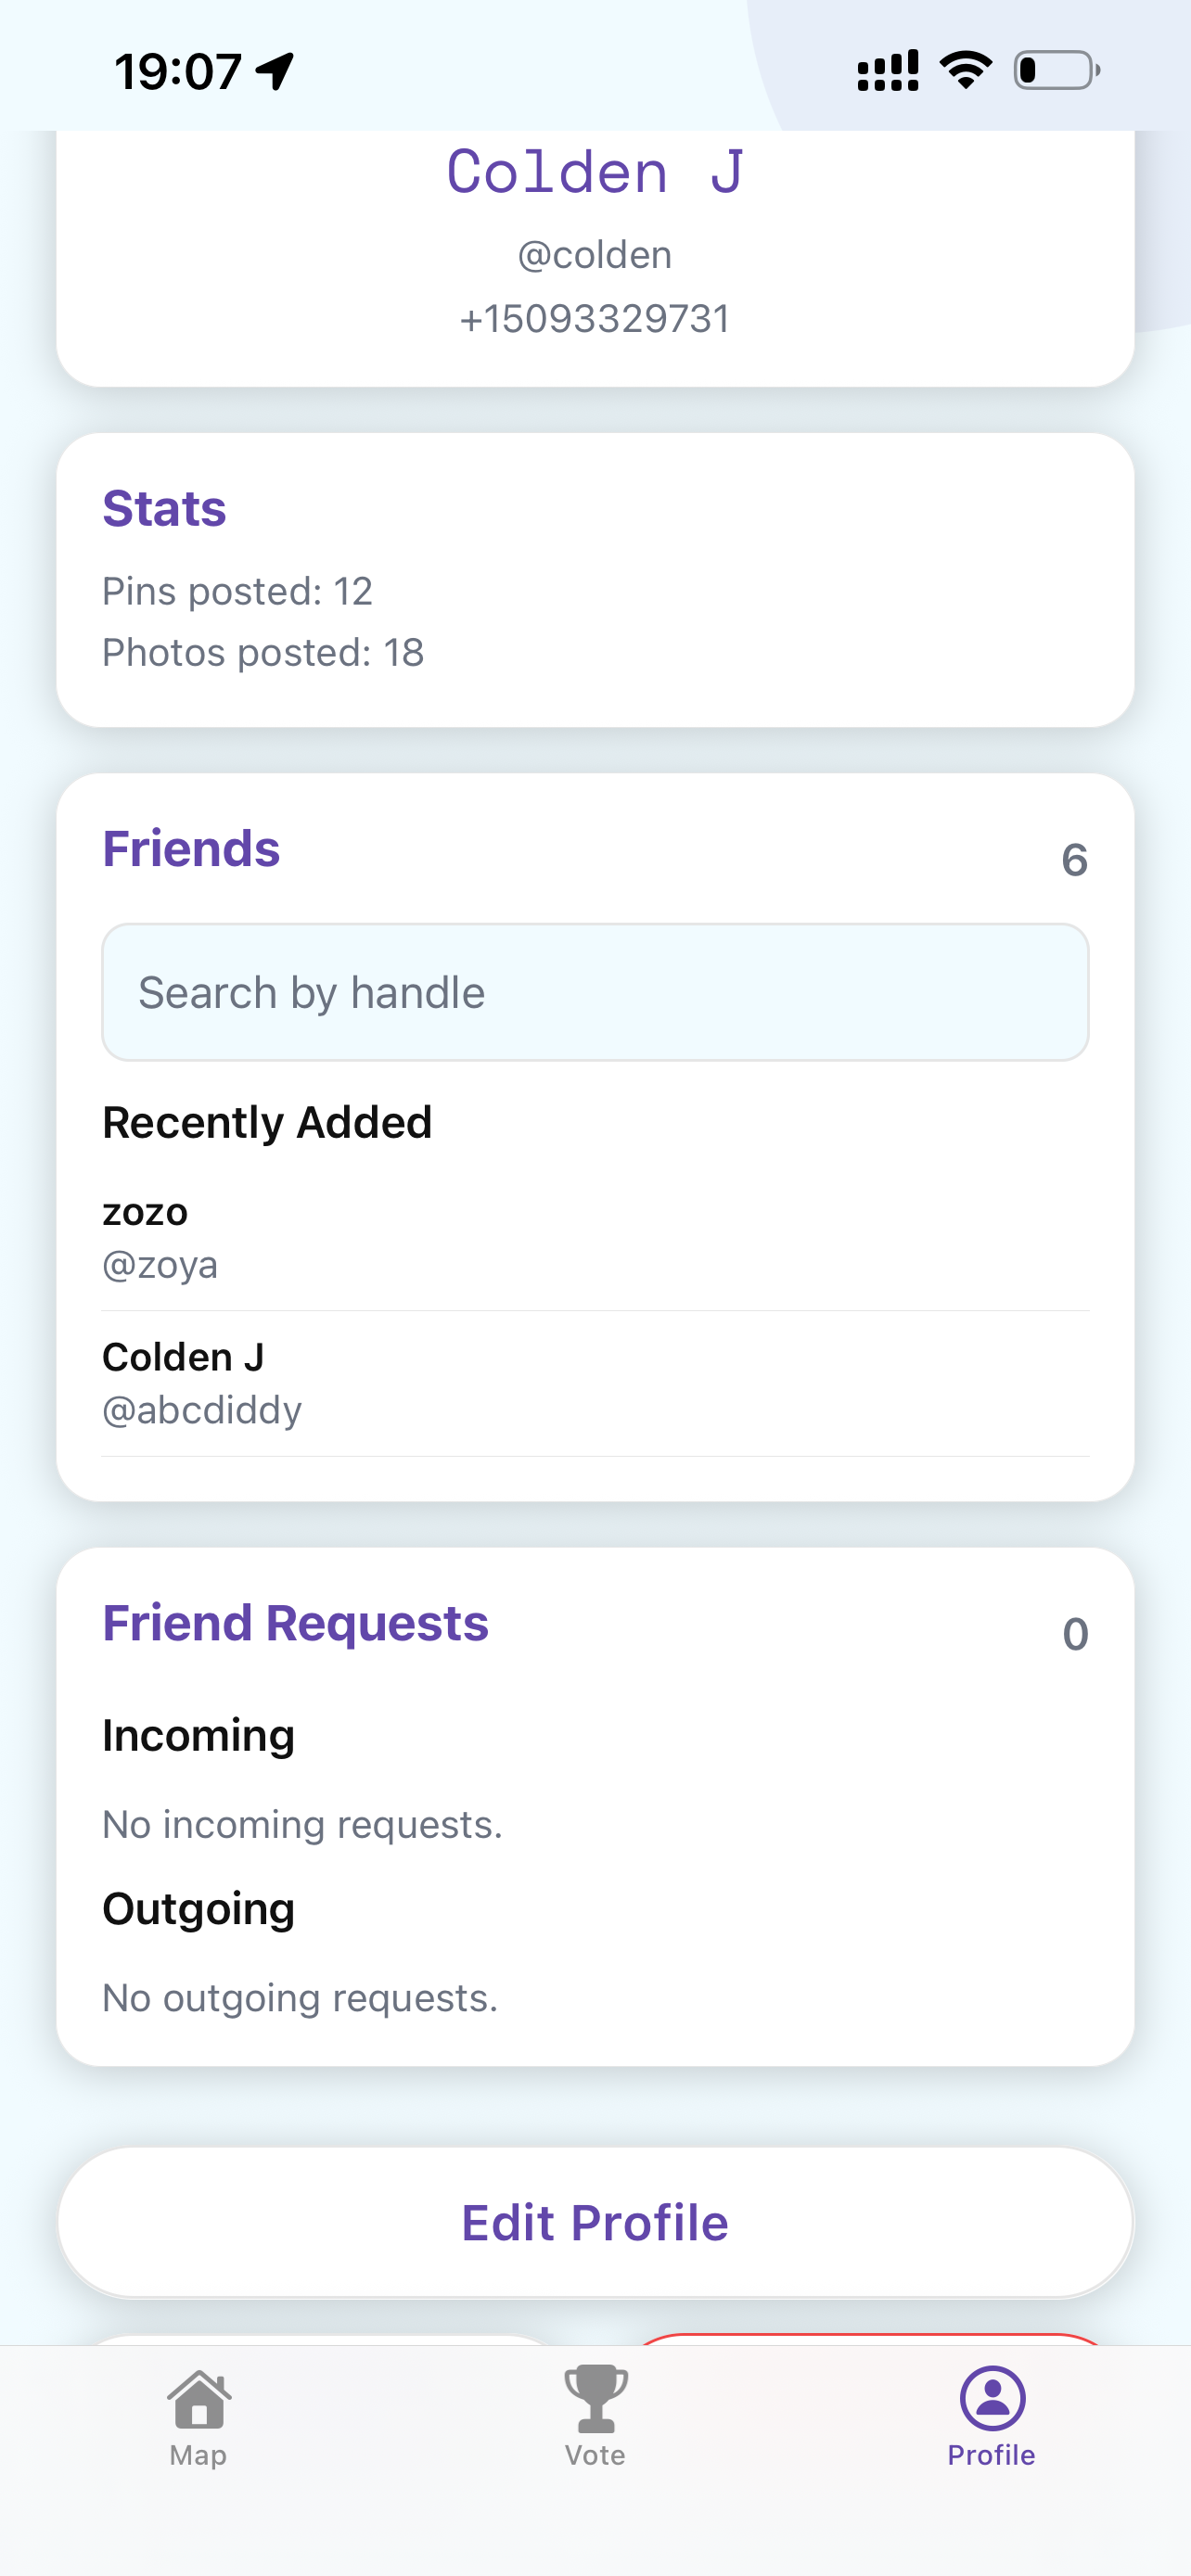
\includegraphics[width=\linewidth]{UserProfile.PNG}
    \caption{User profile with friends. \textit{(Current profile view, showing the friends system and user identity details.)}}
    \label{fig:user-profile}
  \end{minipage}
\end{figure}

\begin{figure}[!htbp]
  \centering
  \begin{minipage}[t]{0.48\linewidth}
    \centering
    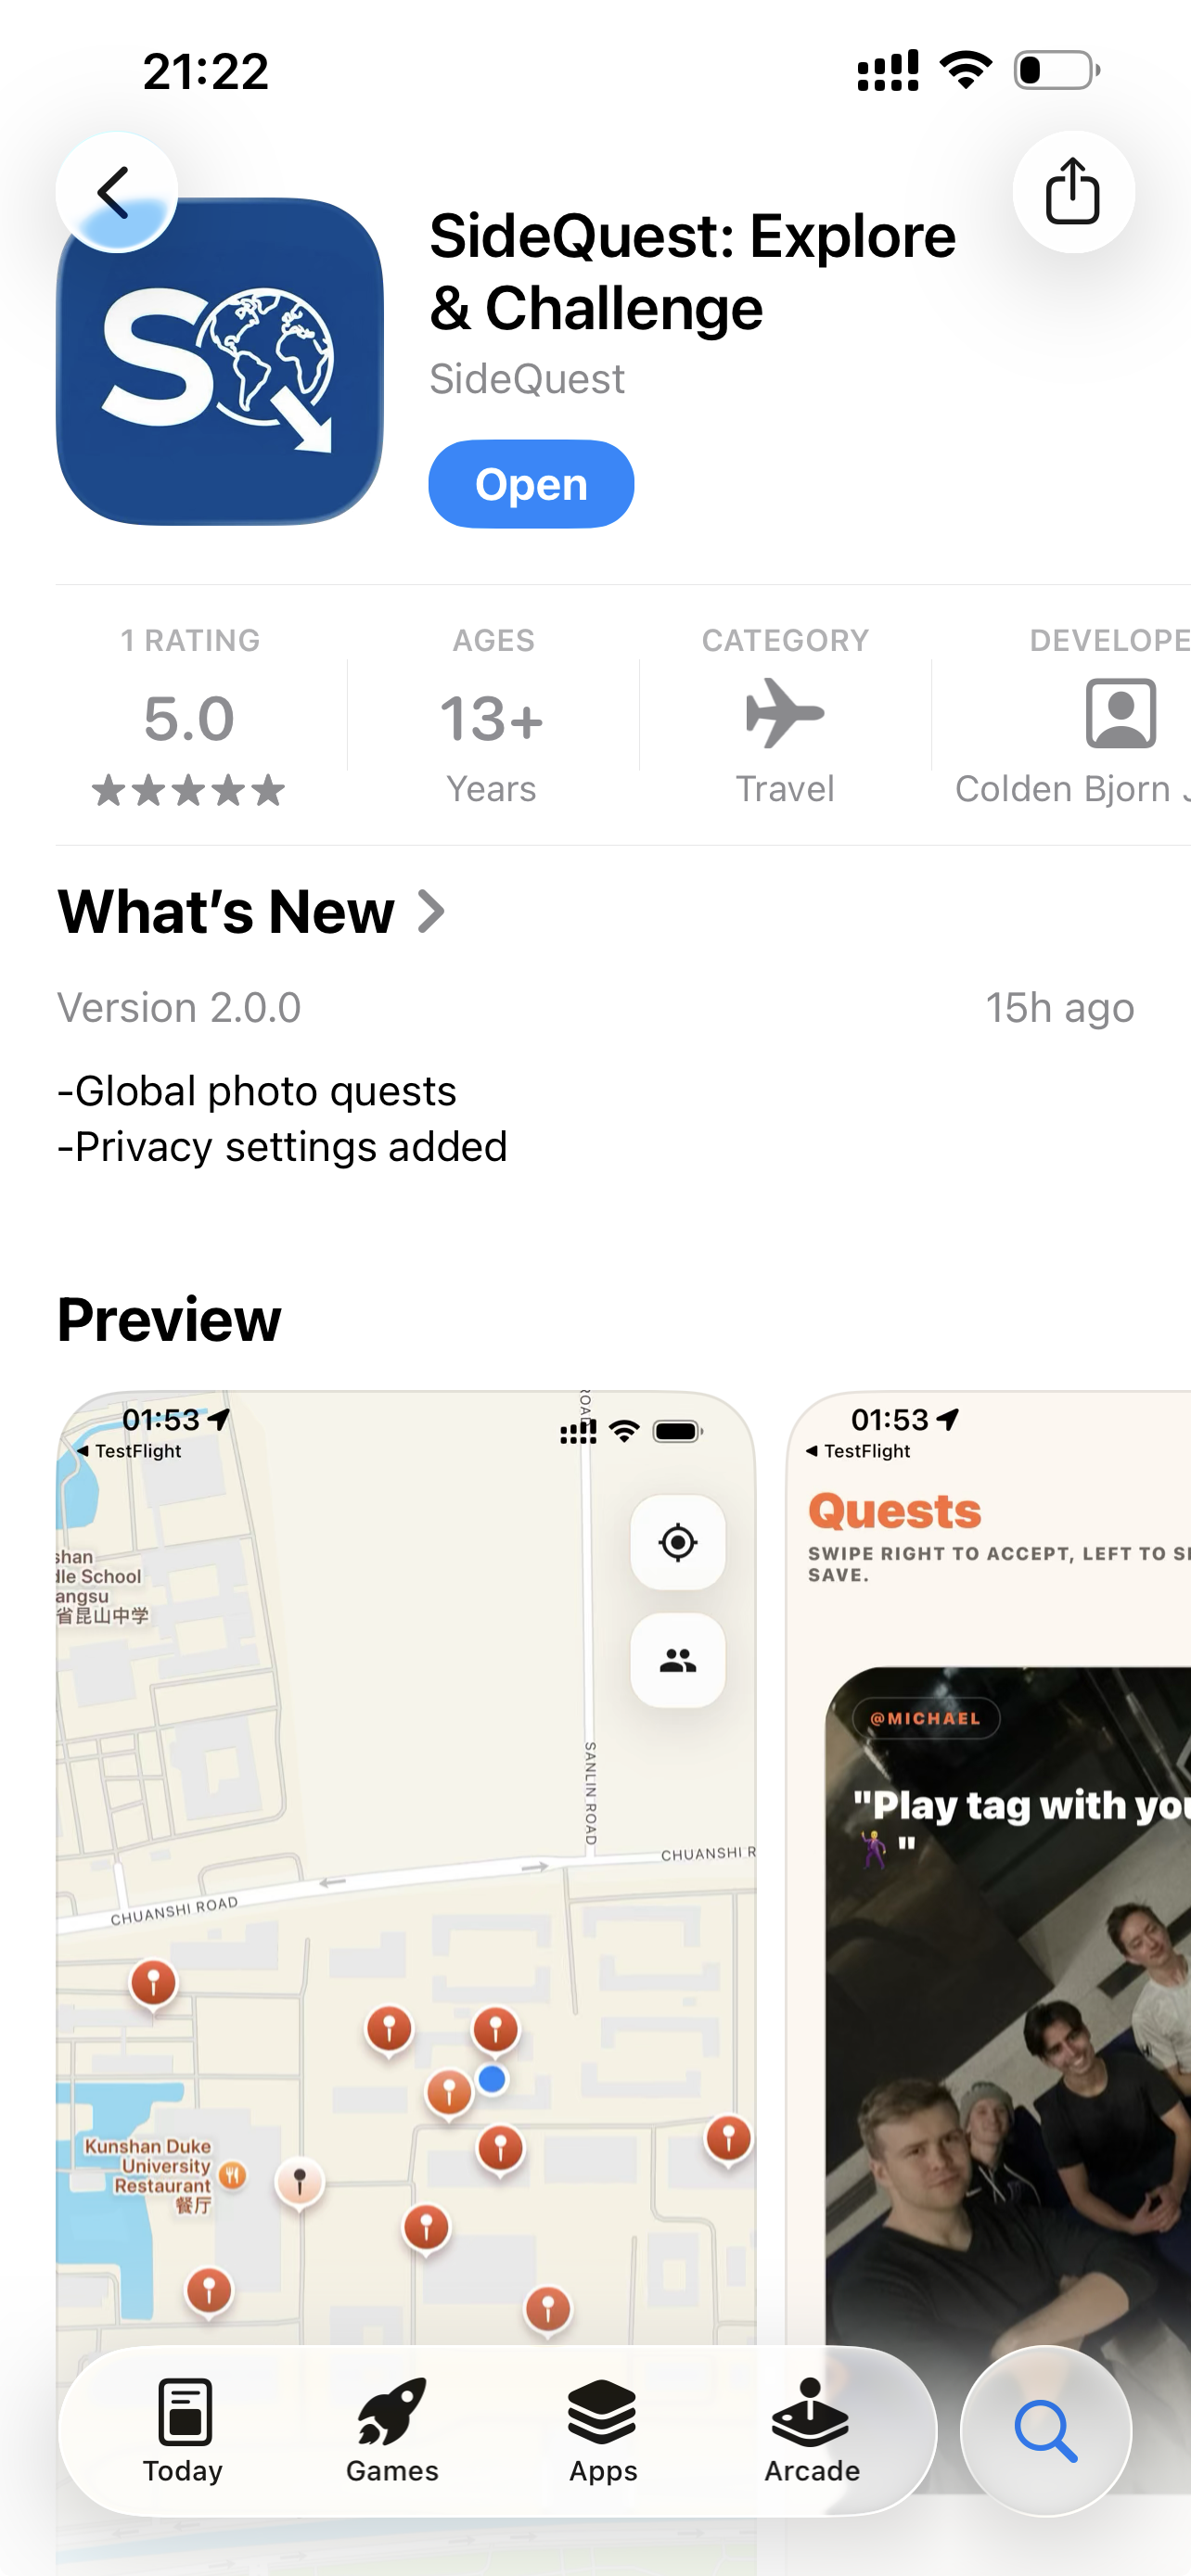
\includegraphics[width=\linewidth]{AppPhotos/sidequest_appstorepage.png}
    \caption{SideQuest App Store page. \textit{(Public listing for SideQuest: Explore \& Challenge.)}}
    \label{fig:appphotos-appstore-page}
  \end{minipage}\hfill
  \begin{minipage}[t]{0.48\linewidth}
    \centering
    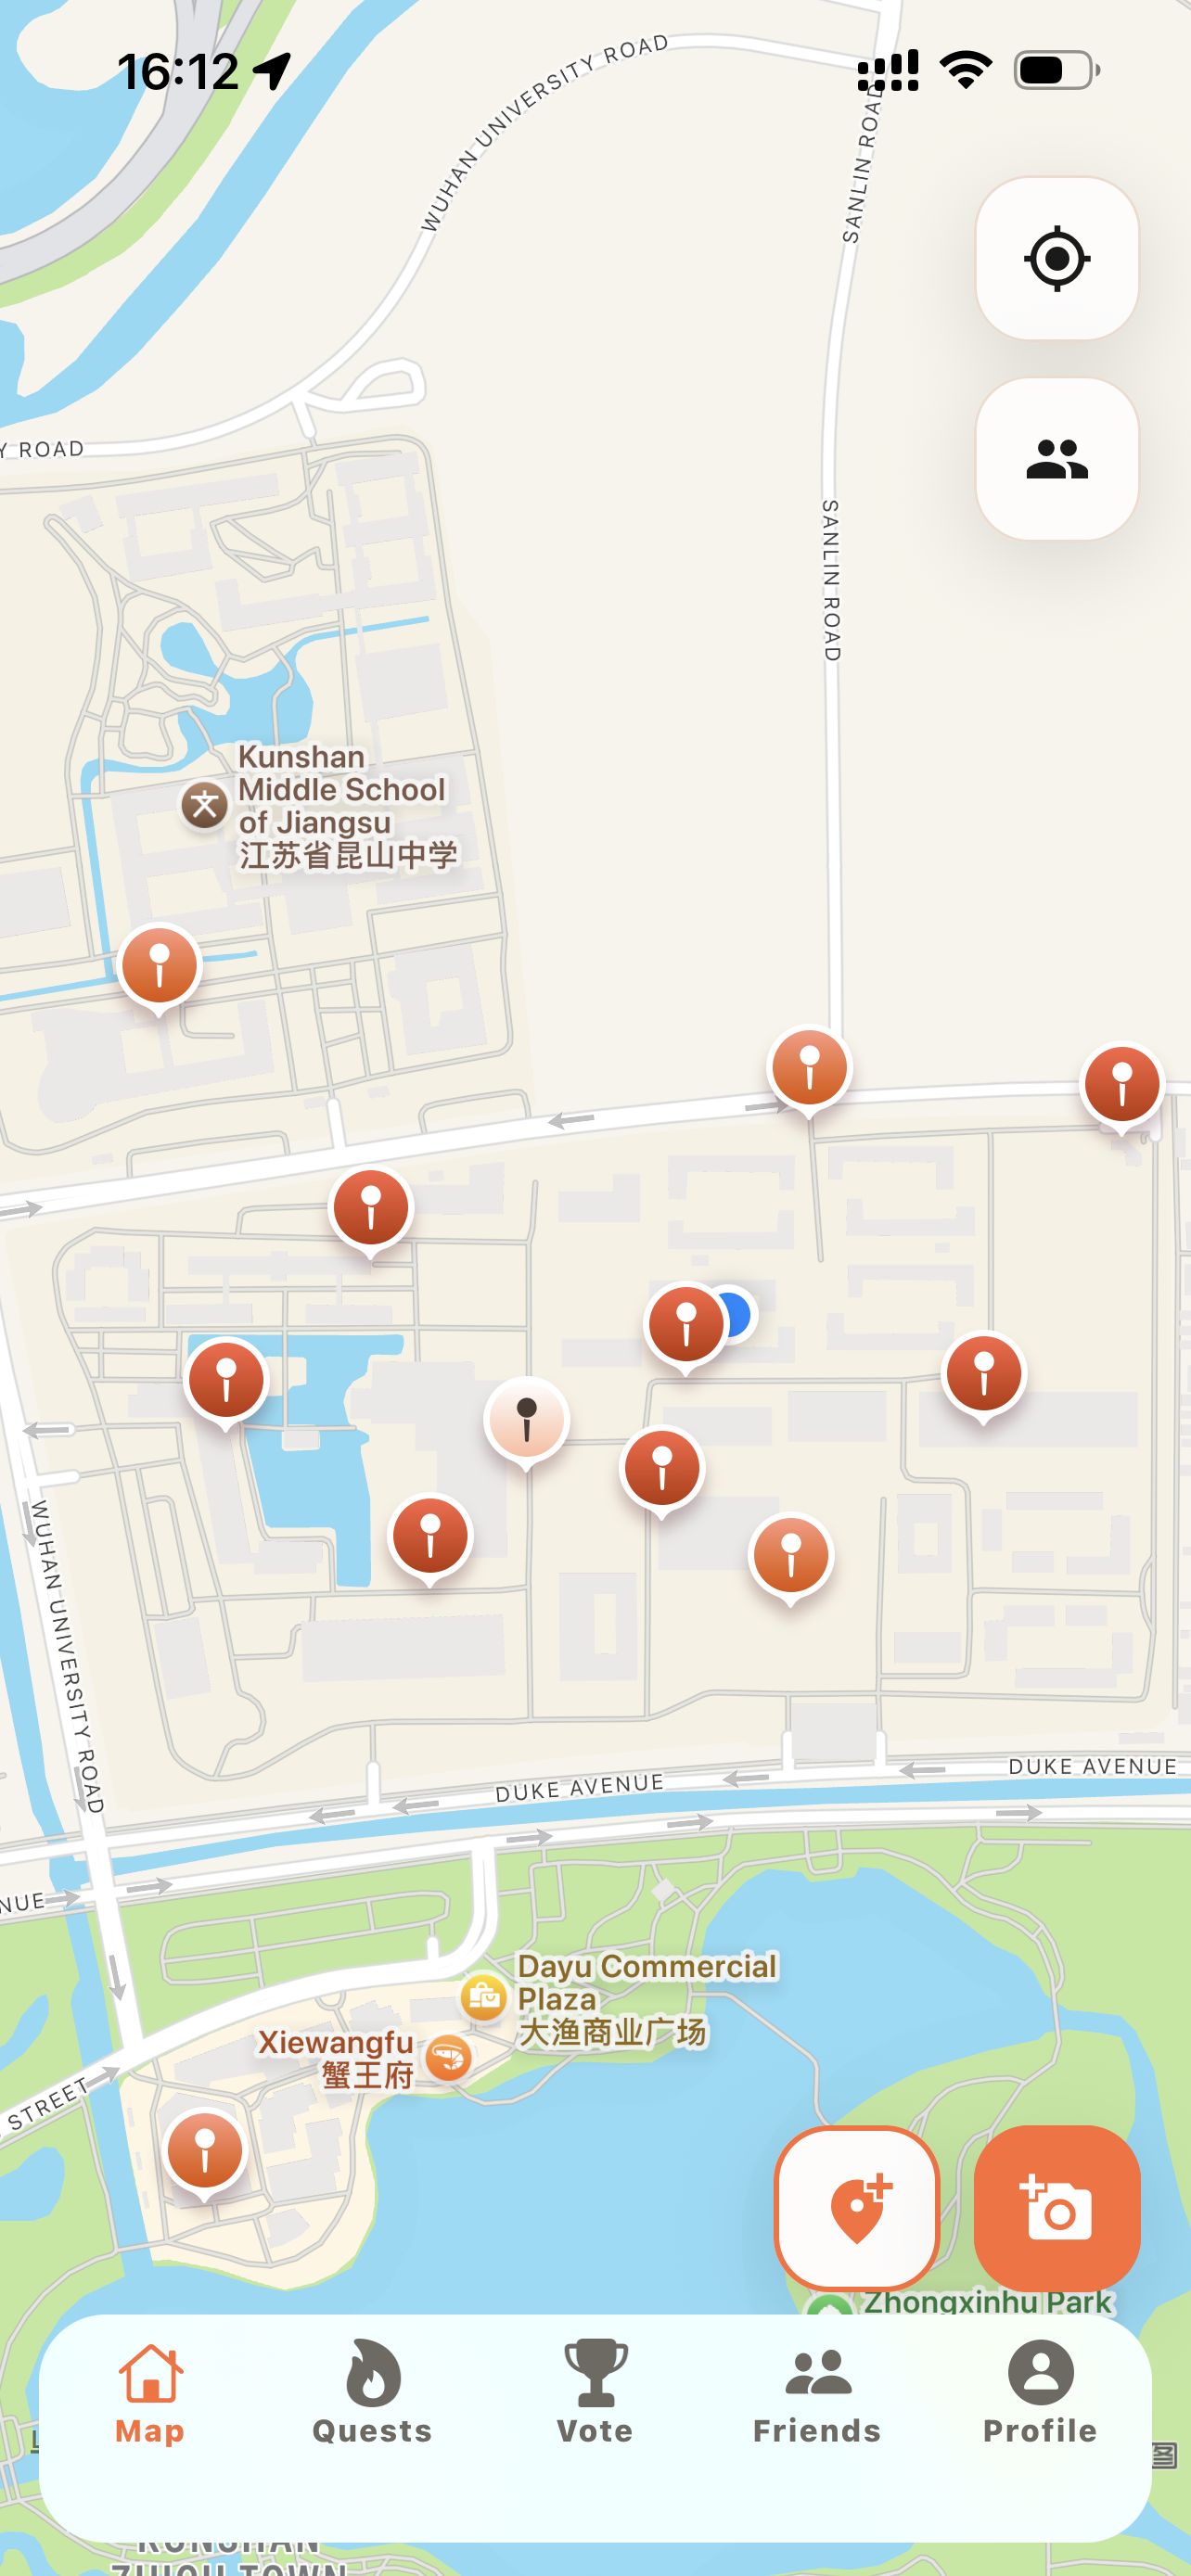
\includegraphics[width=\linewidth]{AppPhotos/Sidequest_Map.PNG}
    \caption{In-app map view. \textit{(Primary live map screen used to discover nearby Quests.)}}
    \label{fig:appphotos-map}
  \end{minipage}
\end{figure}

\begin{figure}[!htbp]
  \centering
  \begin{minipage}[t]{0.48\linewidth}
    \centering
    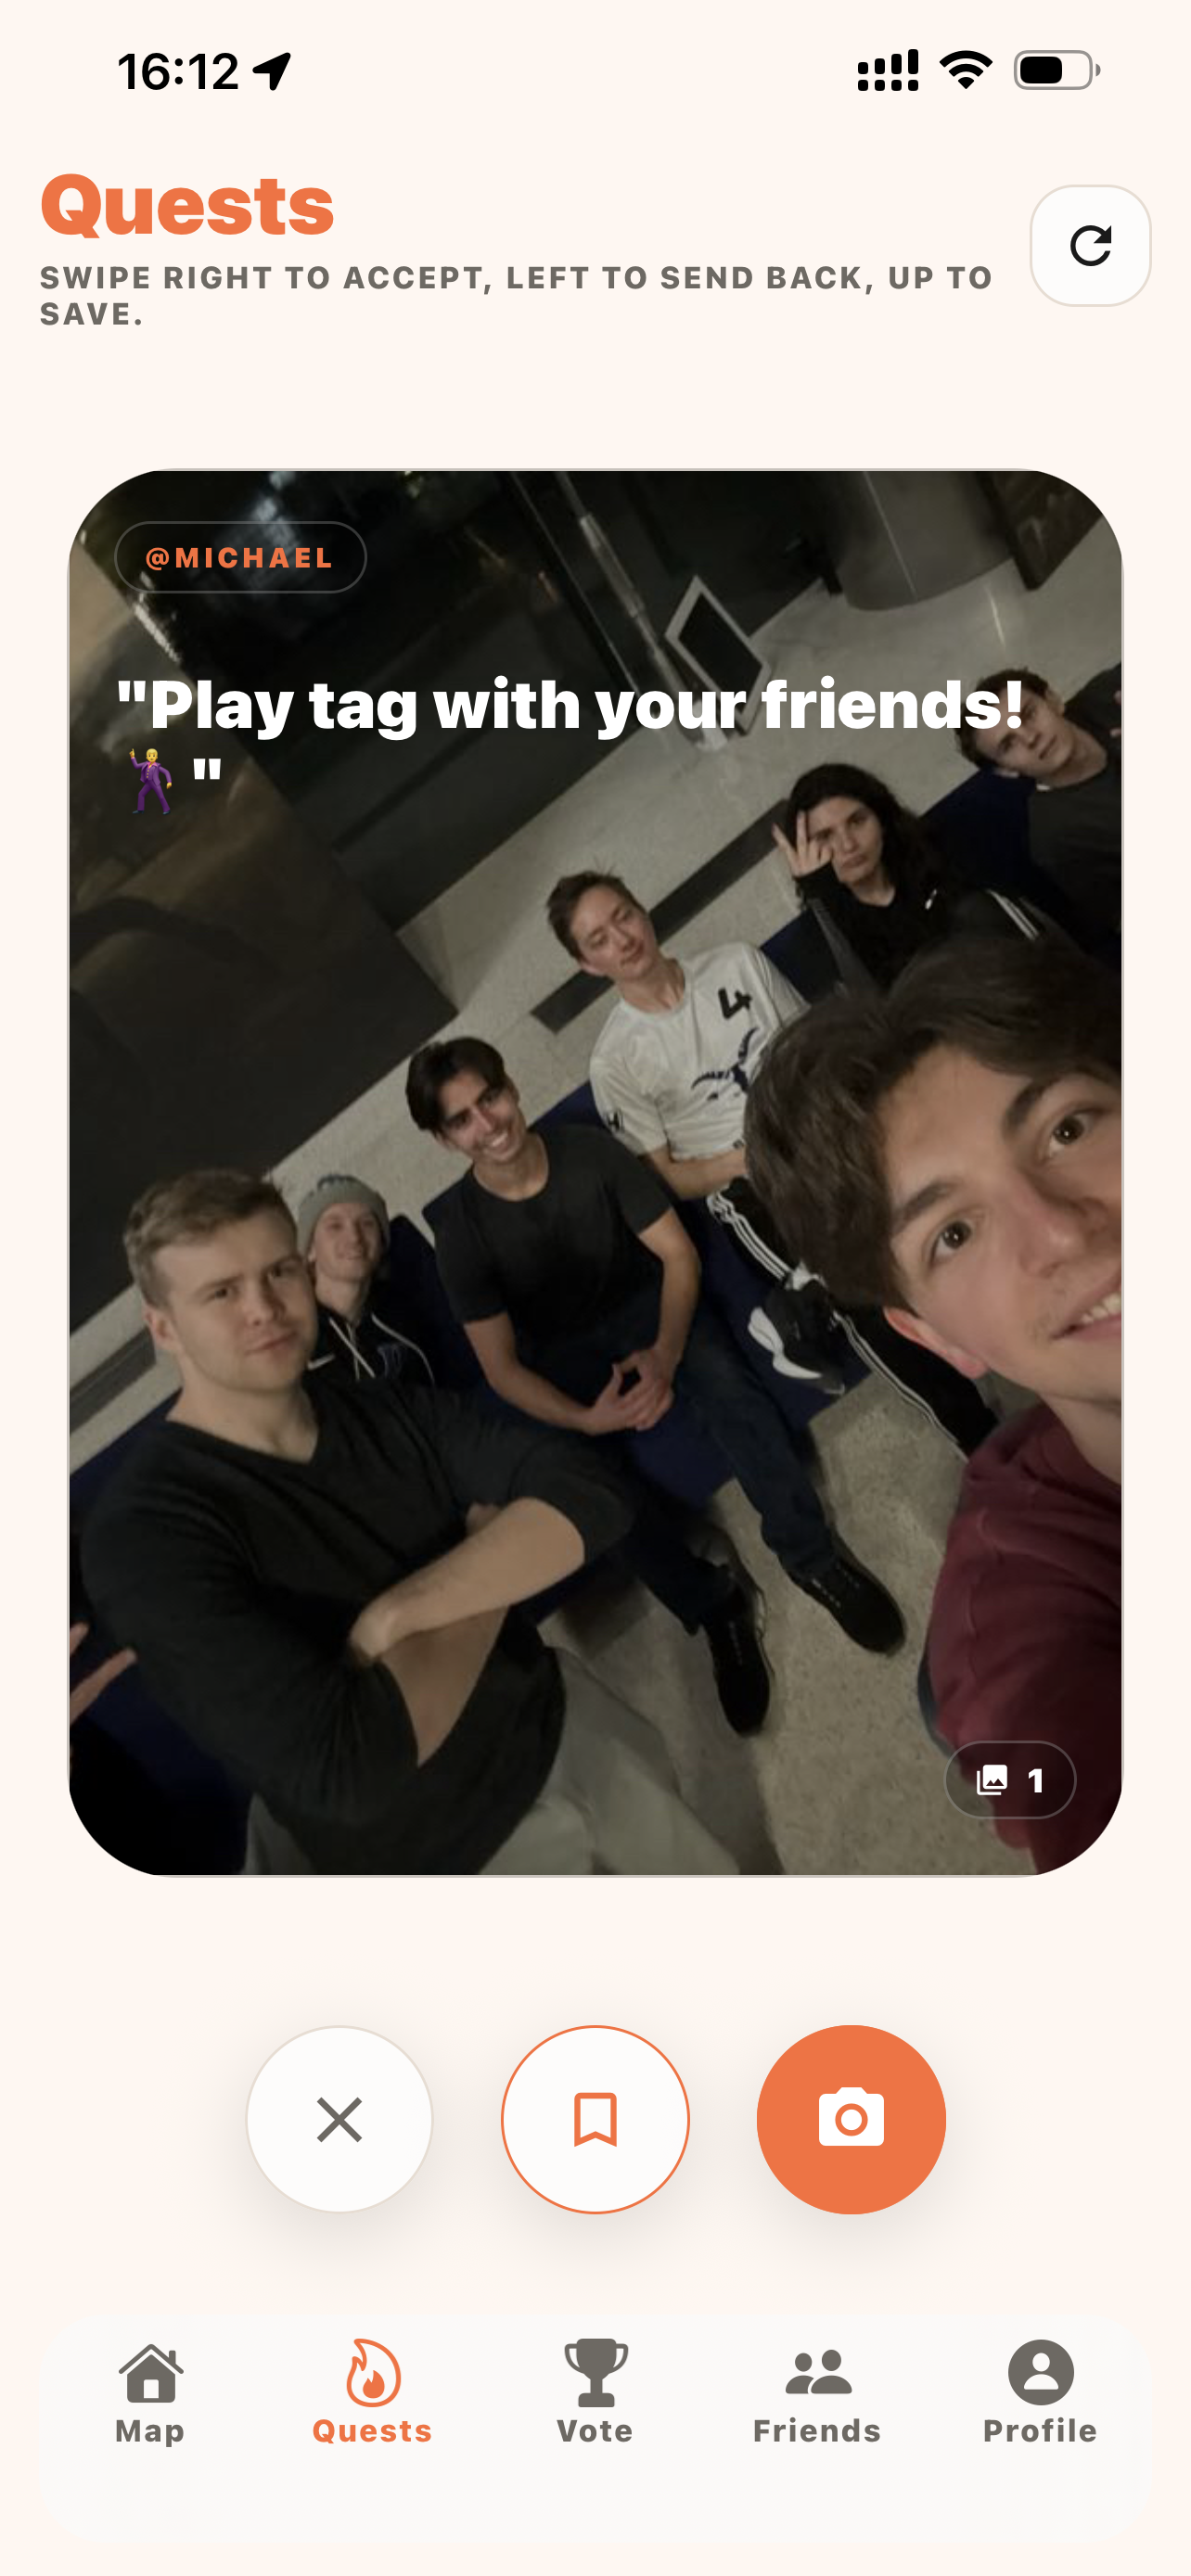
\includegraphics[width=\linewidth]{AppPhotos/Sidequest_Quests.PNG}
    \caption{Quests feed view. \textit{(Quest browsing interface for challenge discovery and participation.)}}
    \label{fig:appphotos-quests}
  \end{minipage}\hfill
  \begin{minipage}[t]{0.48\linewidth}
    \centering
    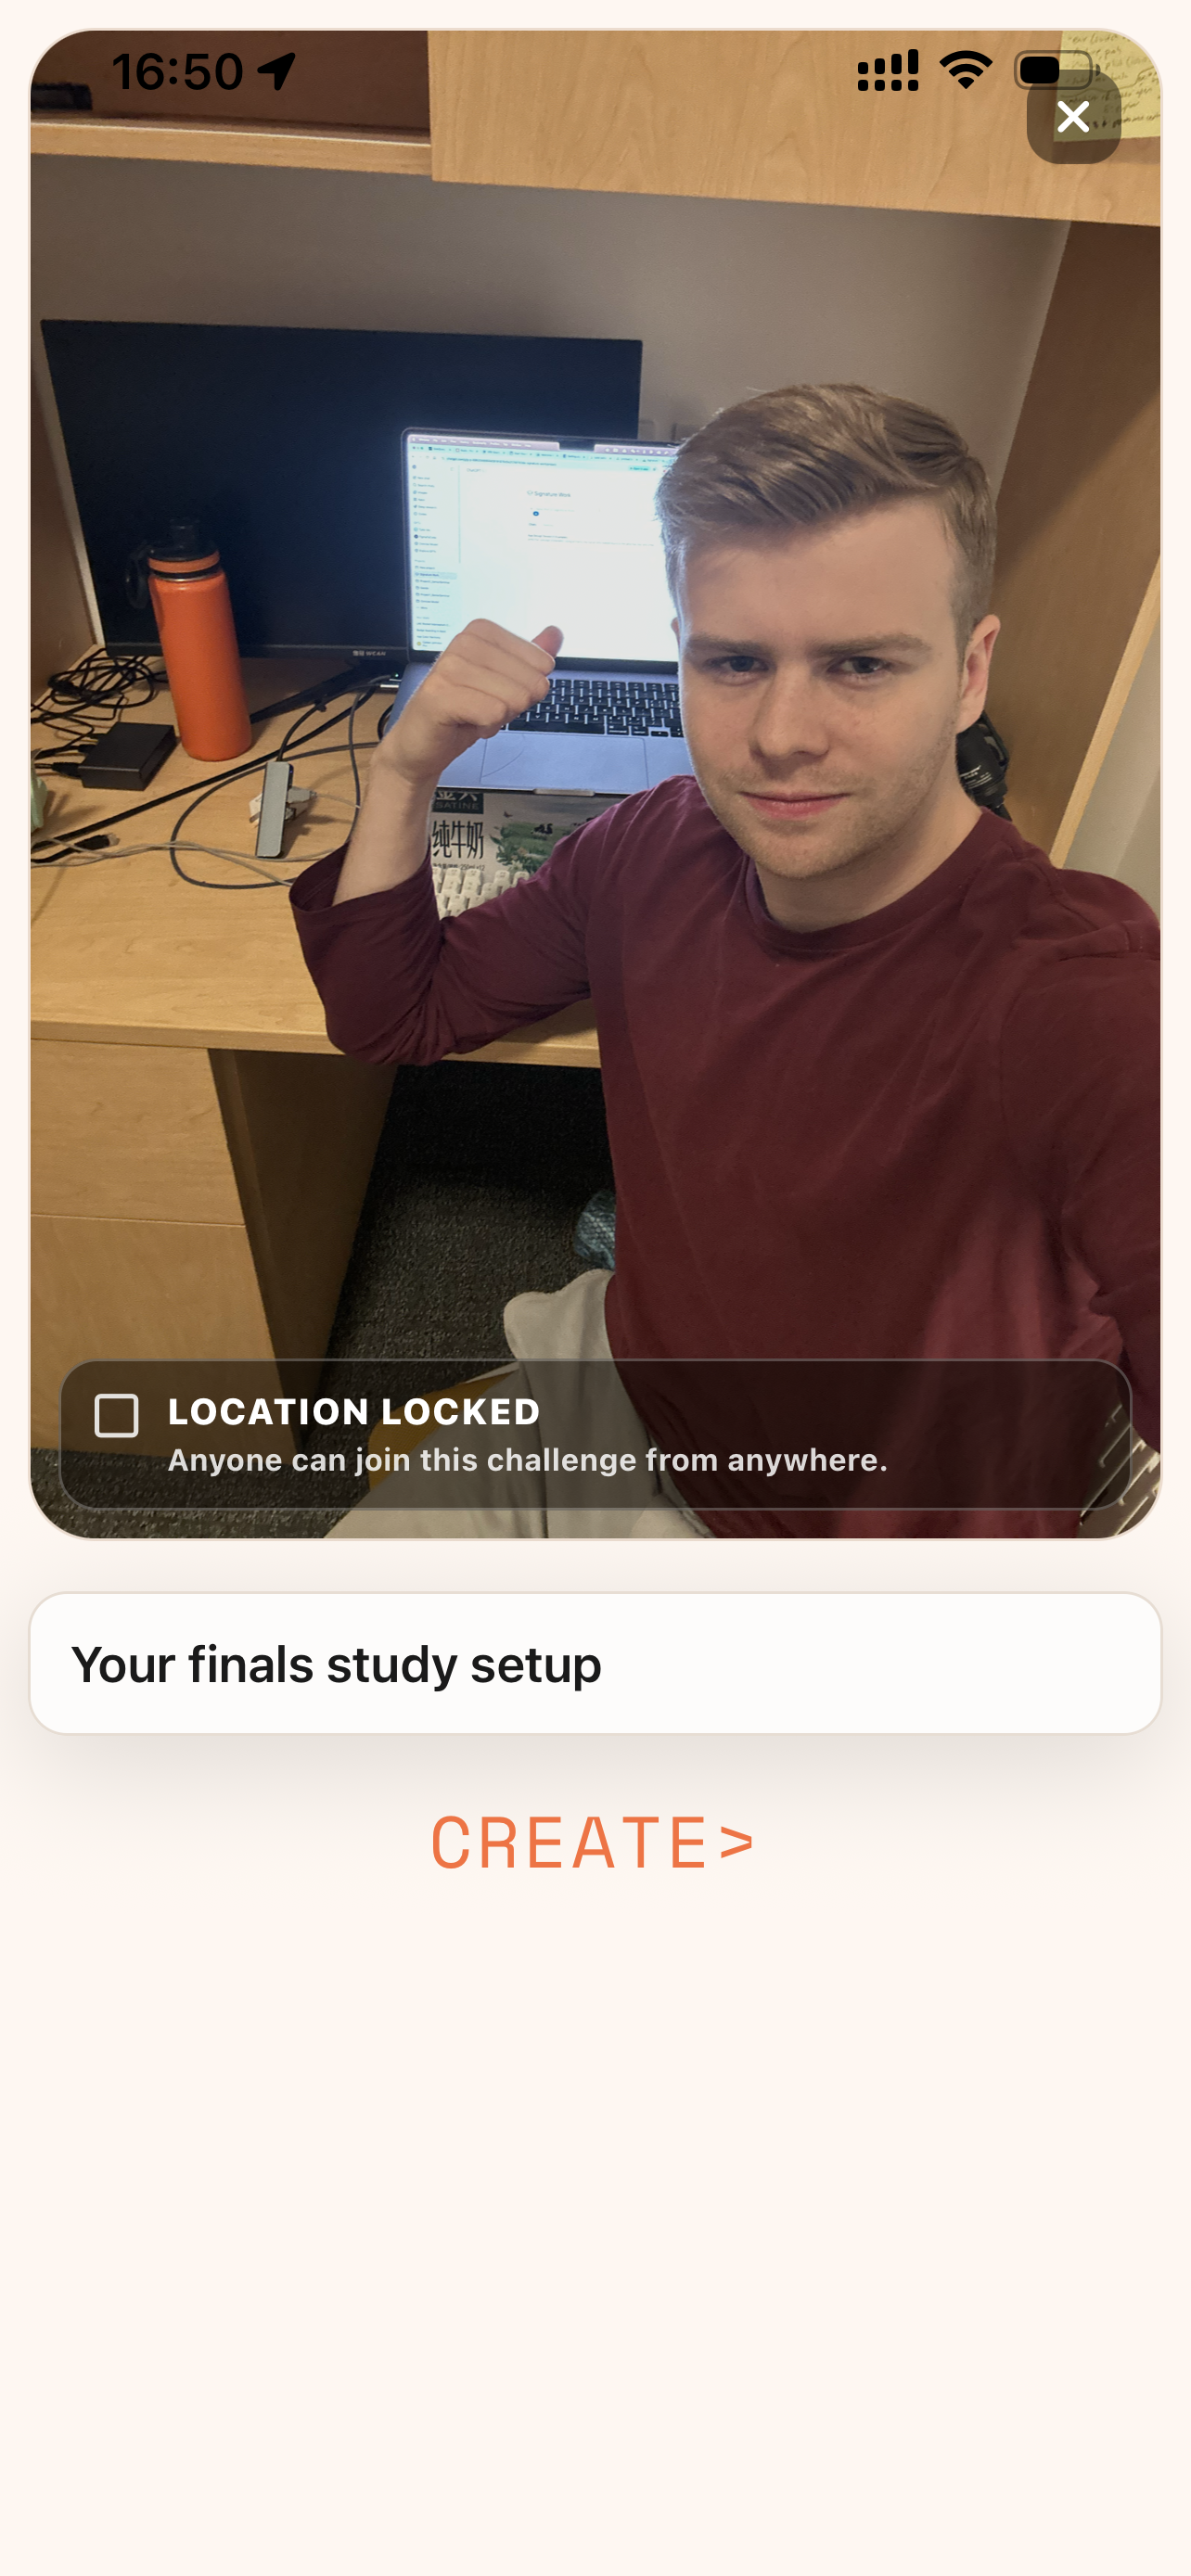
\includegraphics[width=\linewidth]{AppPhotos/Sidequest_ChallengeCreation.PNG}
    \caption{Challenge creation flow. \textit{(UI for creating a new Quest with image and prompt.)}}
    \label{fig:appphotos-challenge-creation}
  \end{minipage}
\end{figure}

\begin{figure}[!htbp]
  \centering
  \begin{minipage}[t]{0.48\linewidth}
    \centering
    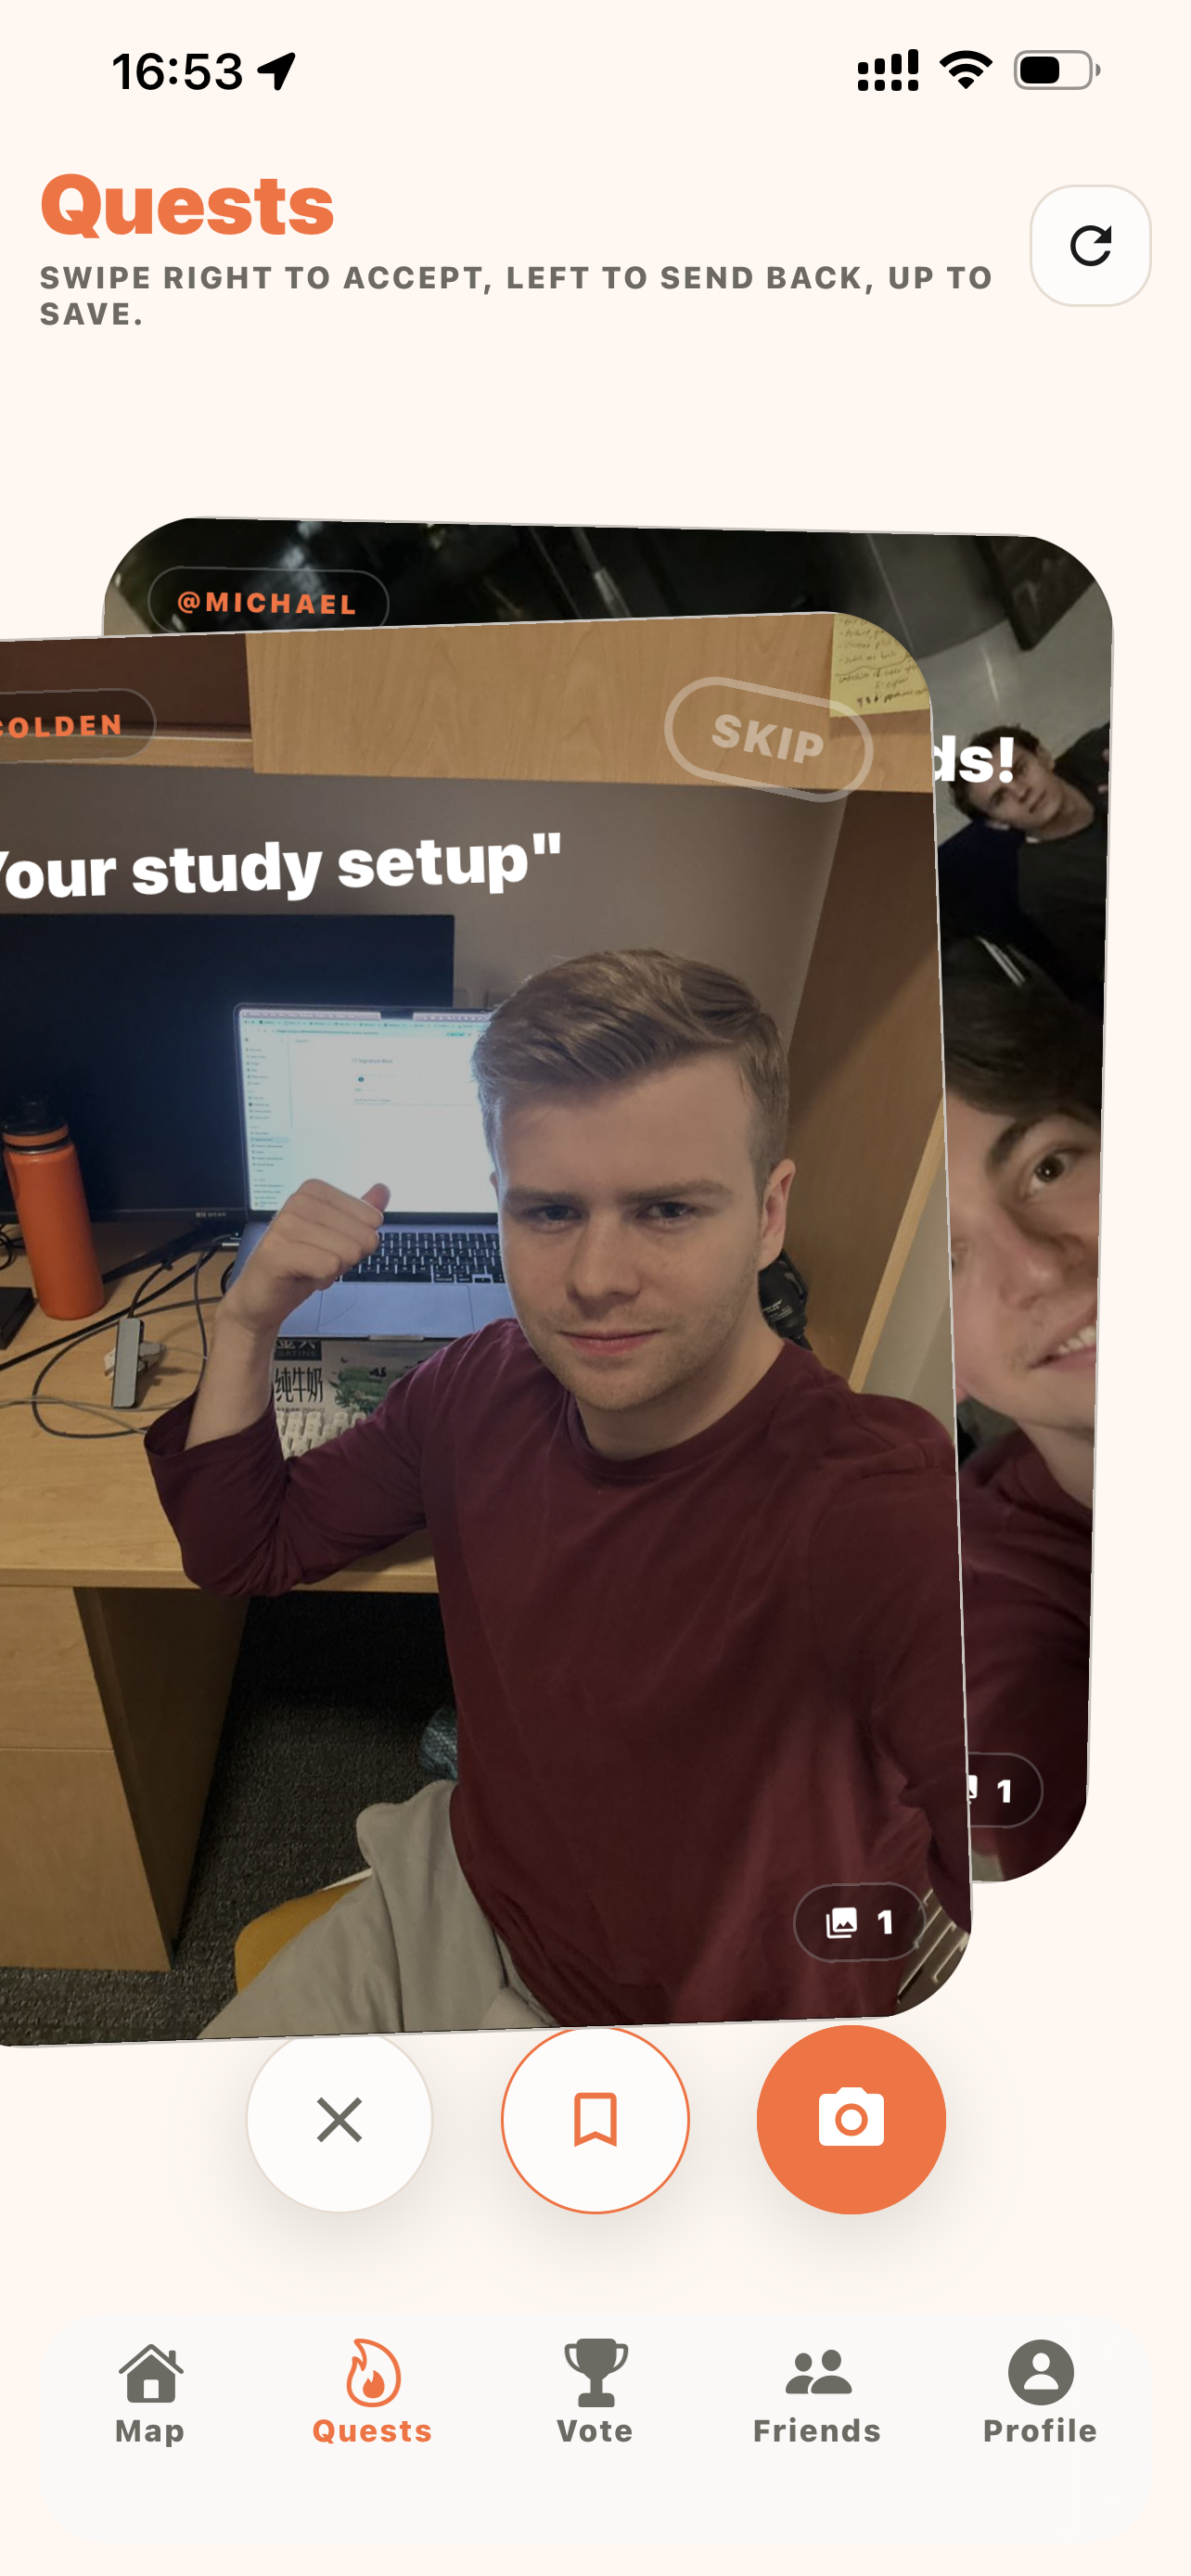
\includegraphics[width=\linewidth]{AppPhotos/SideQuest_ChallengeAppearsinQuests.PNG}
    \caption{Challenge appears in Quest list. \textit{(Newly created challenge surfaced to other users in the feed.)}}
    \label{fig:appphotos-challenge-appears}
  \end{minipage}\hfill
  \begin{minipage}[t]{0.48\linewidth}
    \centering
    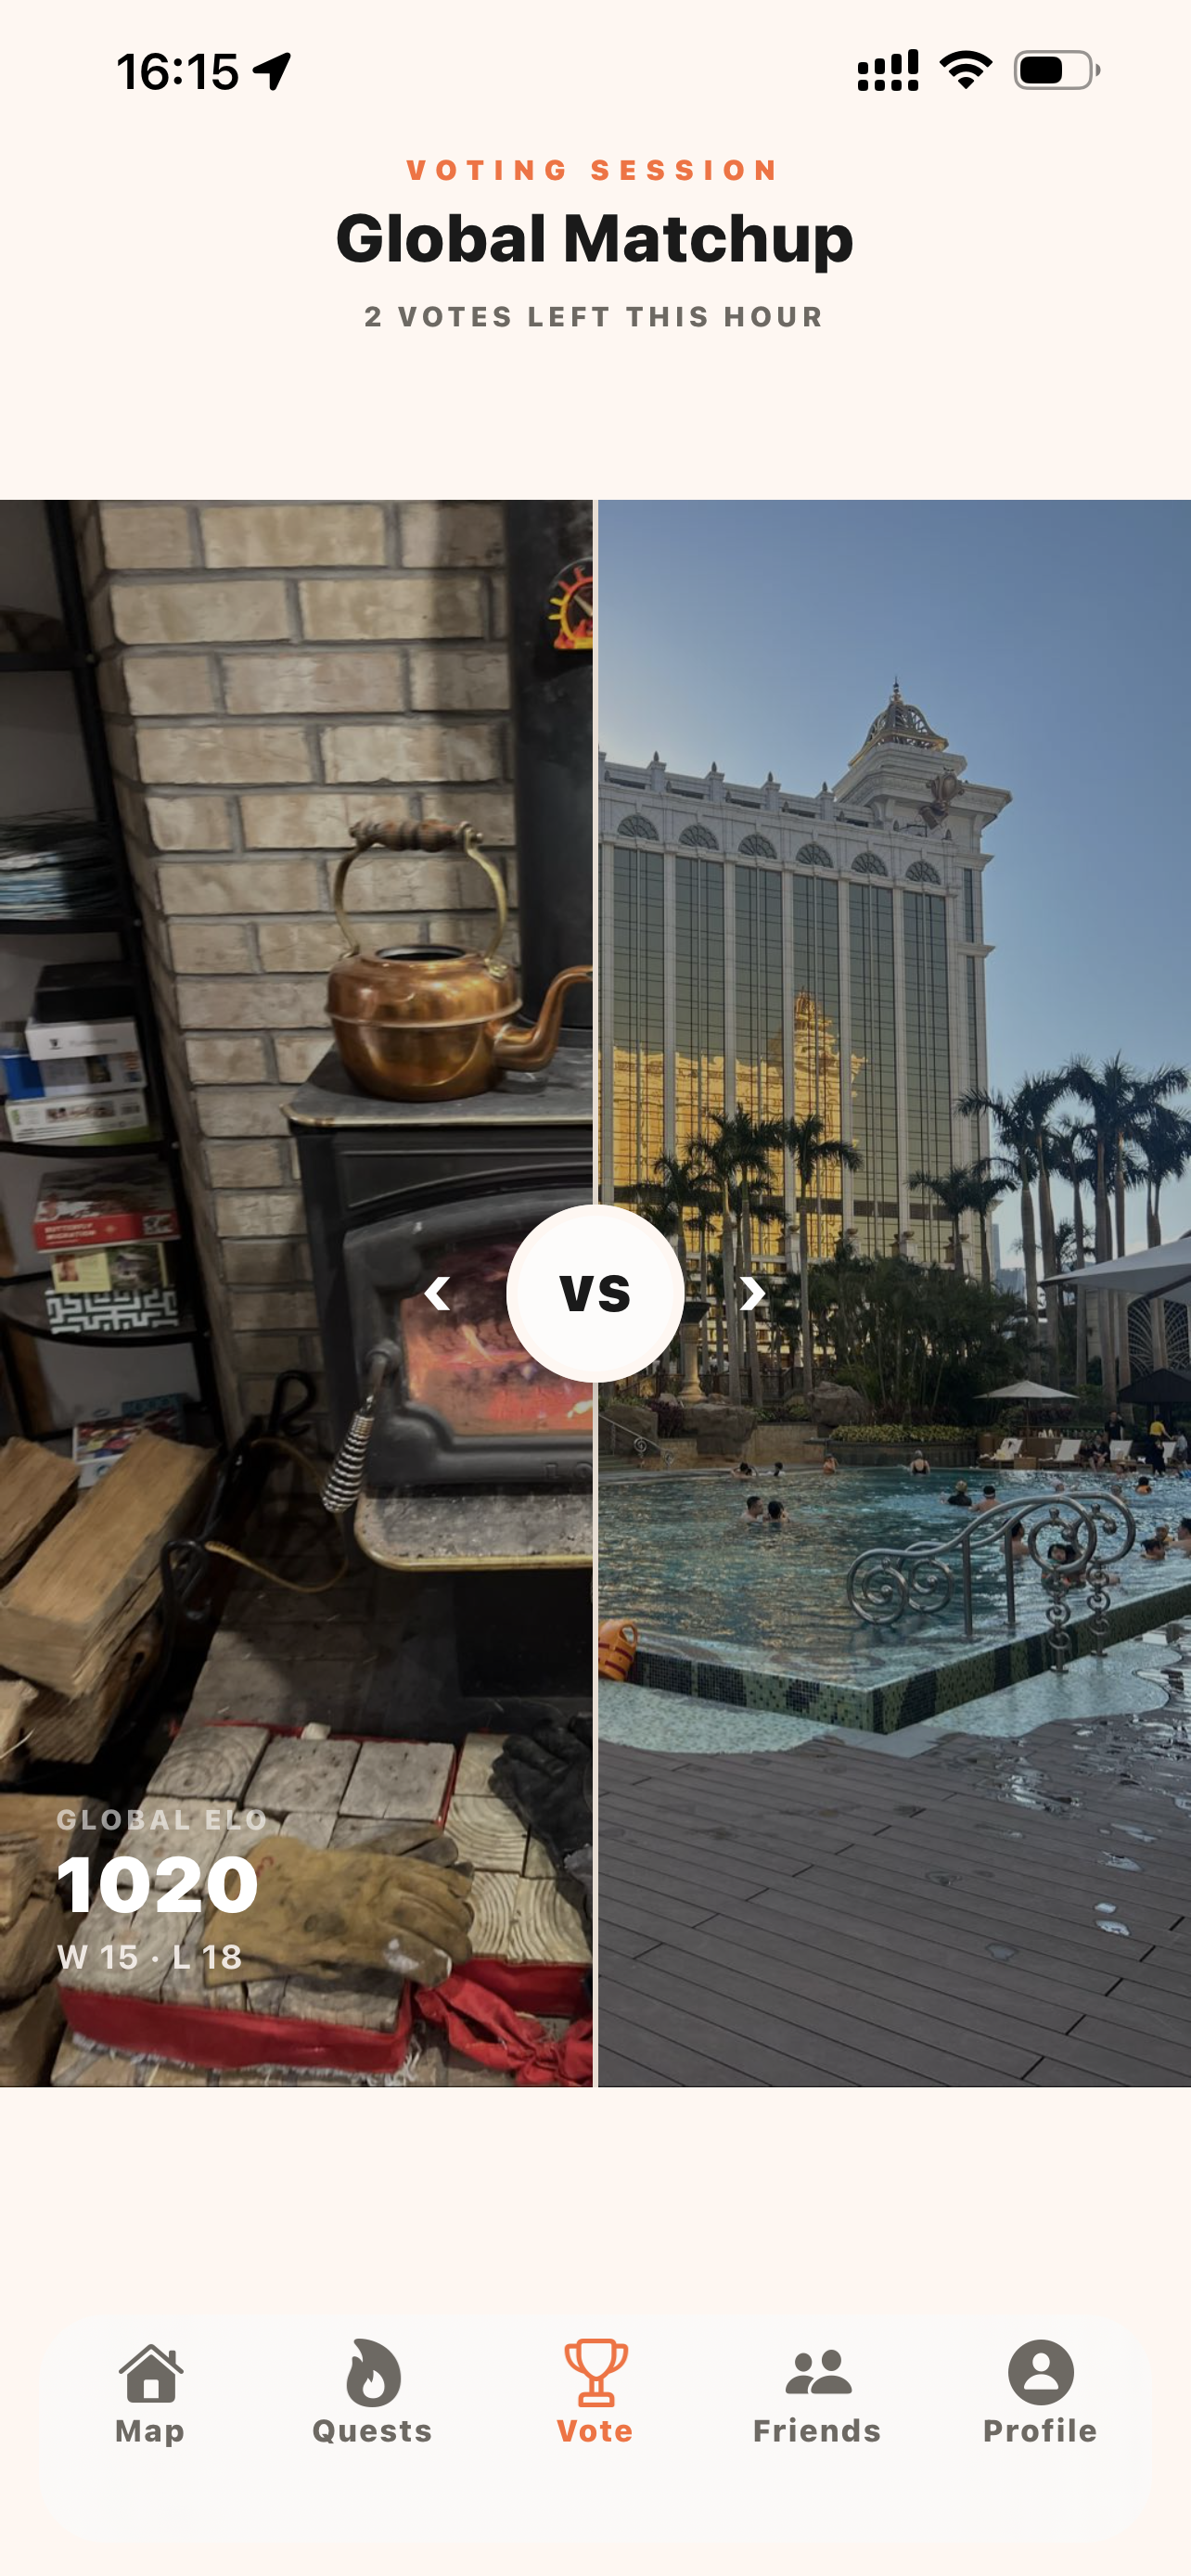
\includegraphics[width=\linewidth]{AppPhotos/Sidequest_voting.PNG}
    \caption{Voting and duel screen. \textit{(Head-to-head voting interface for community ranking.)}}
    \label{fig:appphotos-voting}
  \end{minipage}
\end{figure}

\begin{figure}[!htbp]
  \centering
  \begin{minipage}[t]{0.48\linewidth}
    \centering
    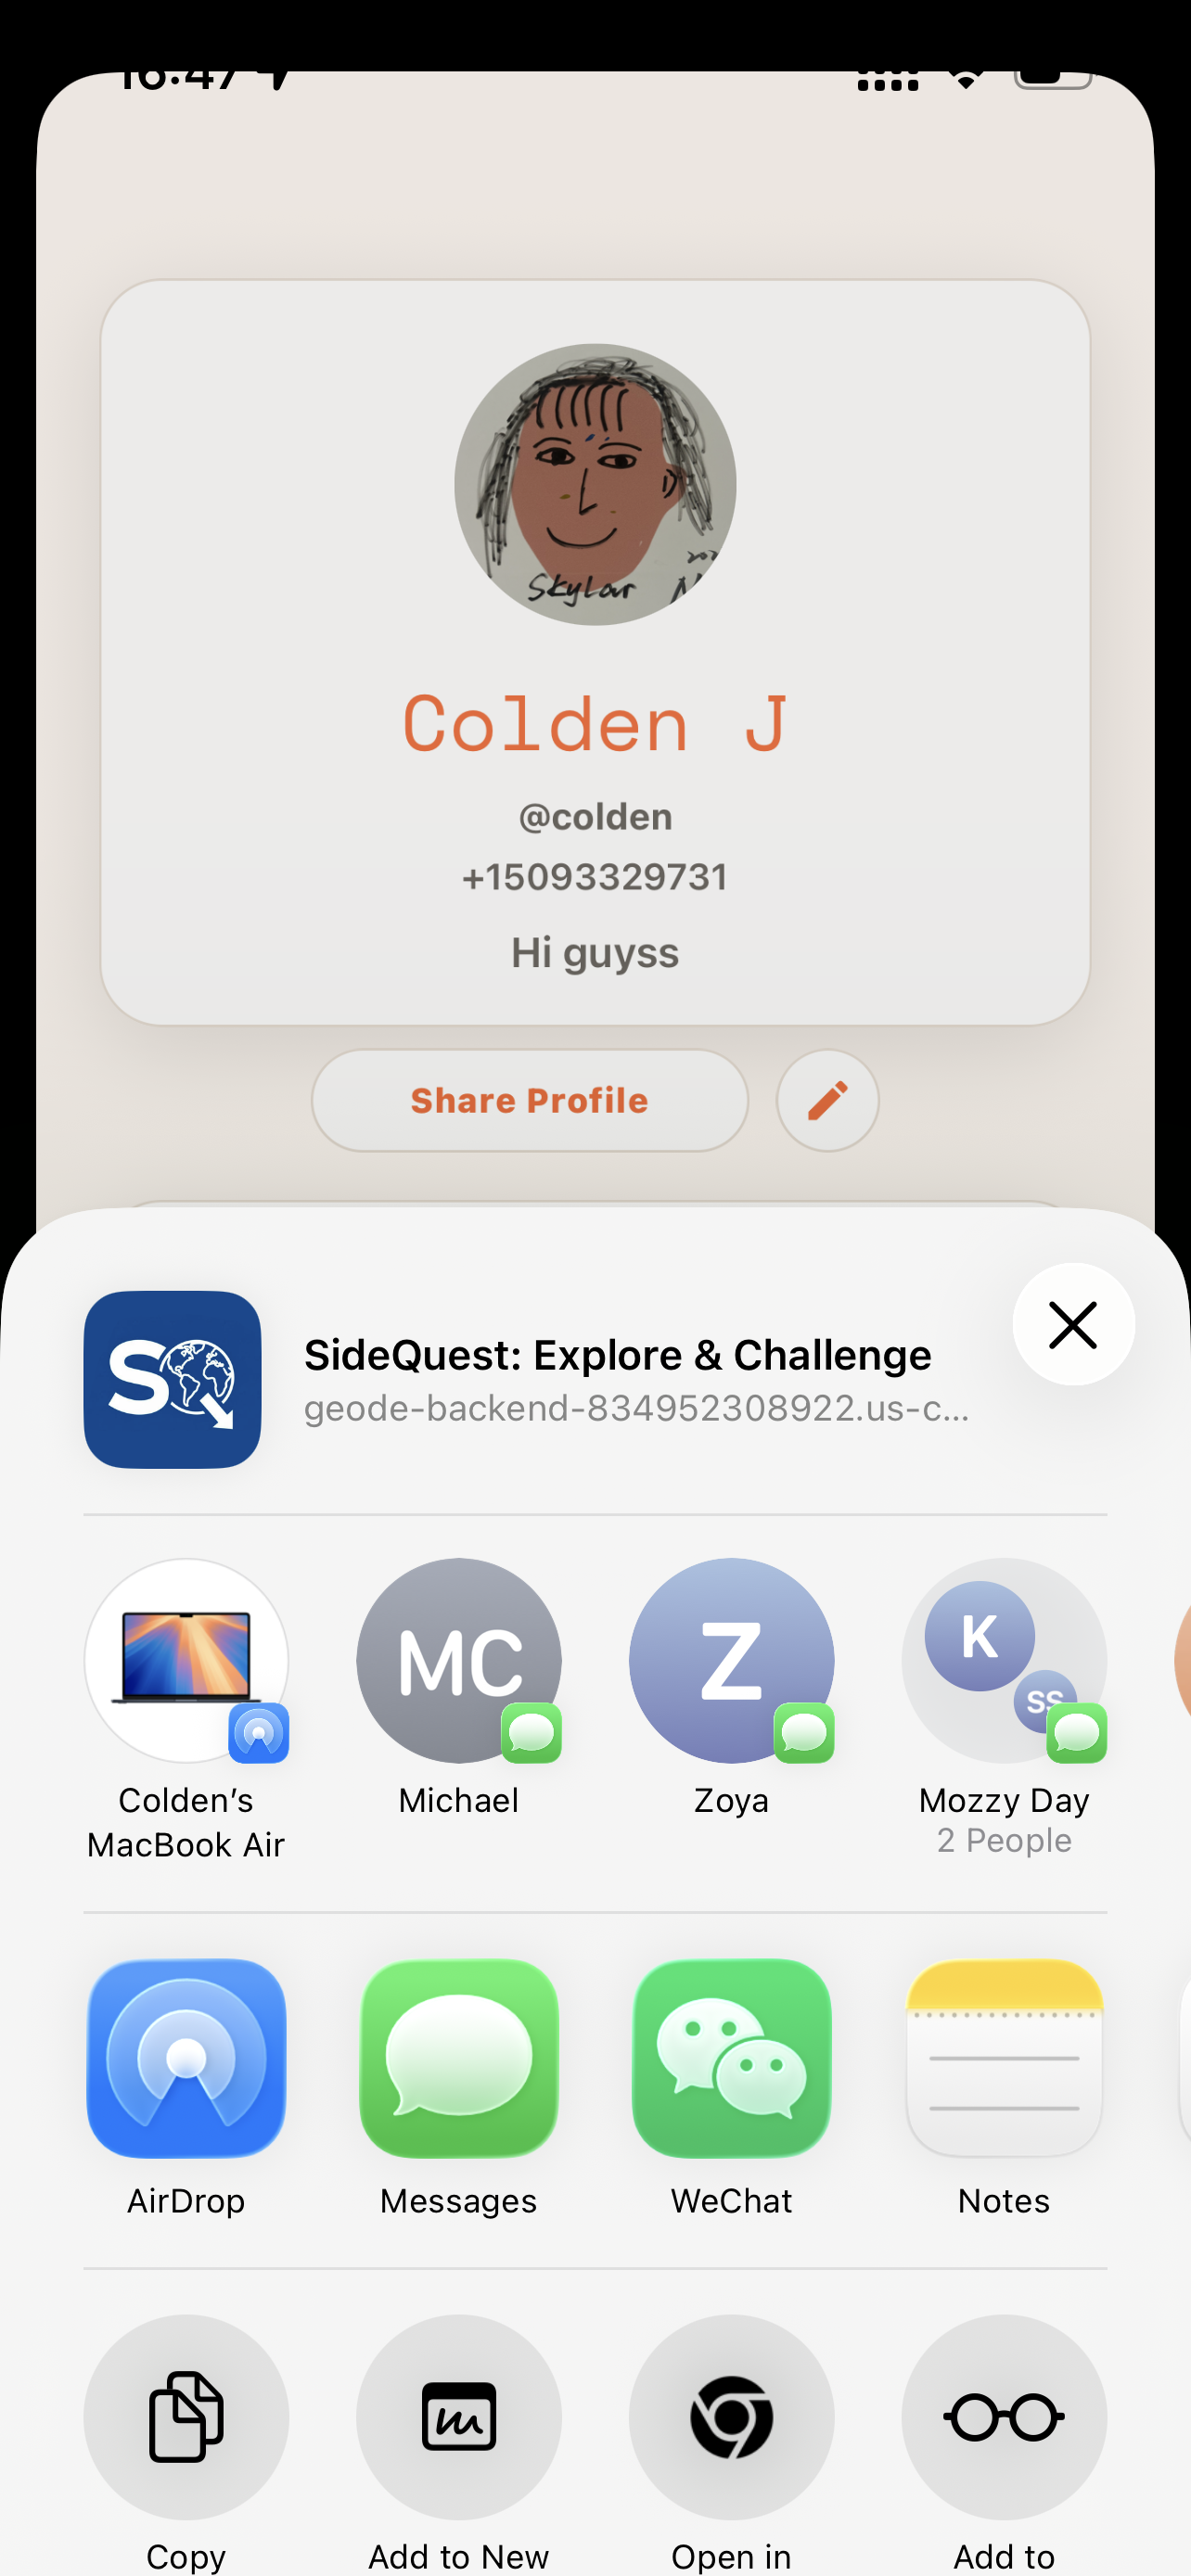
\includegraphics[width=\linewidth]{AppPhotos/Sidequest_Share.PNG}
    \caption{Quest sharing view. \textit{(Sharing interface to distribute challenges with friends.)}}
    \label{fig:appphotos-share}
  \end{minipage}\hfill
  \begin{minipage}[t]{0.48\linewidth}
    \centering
    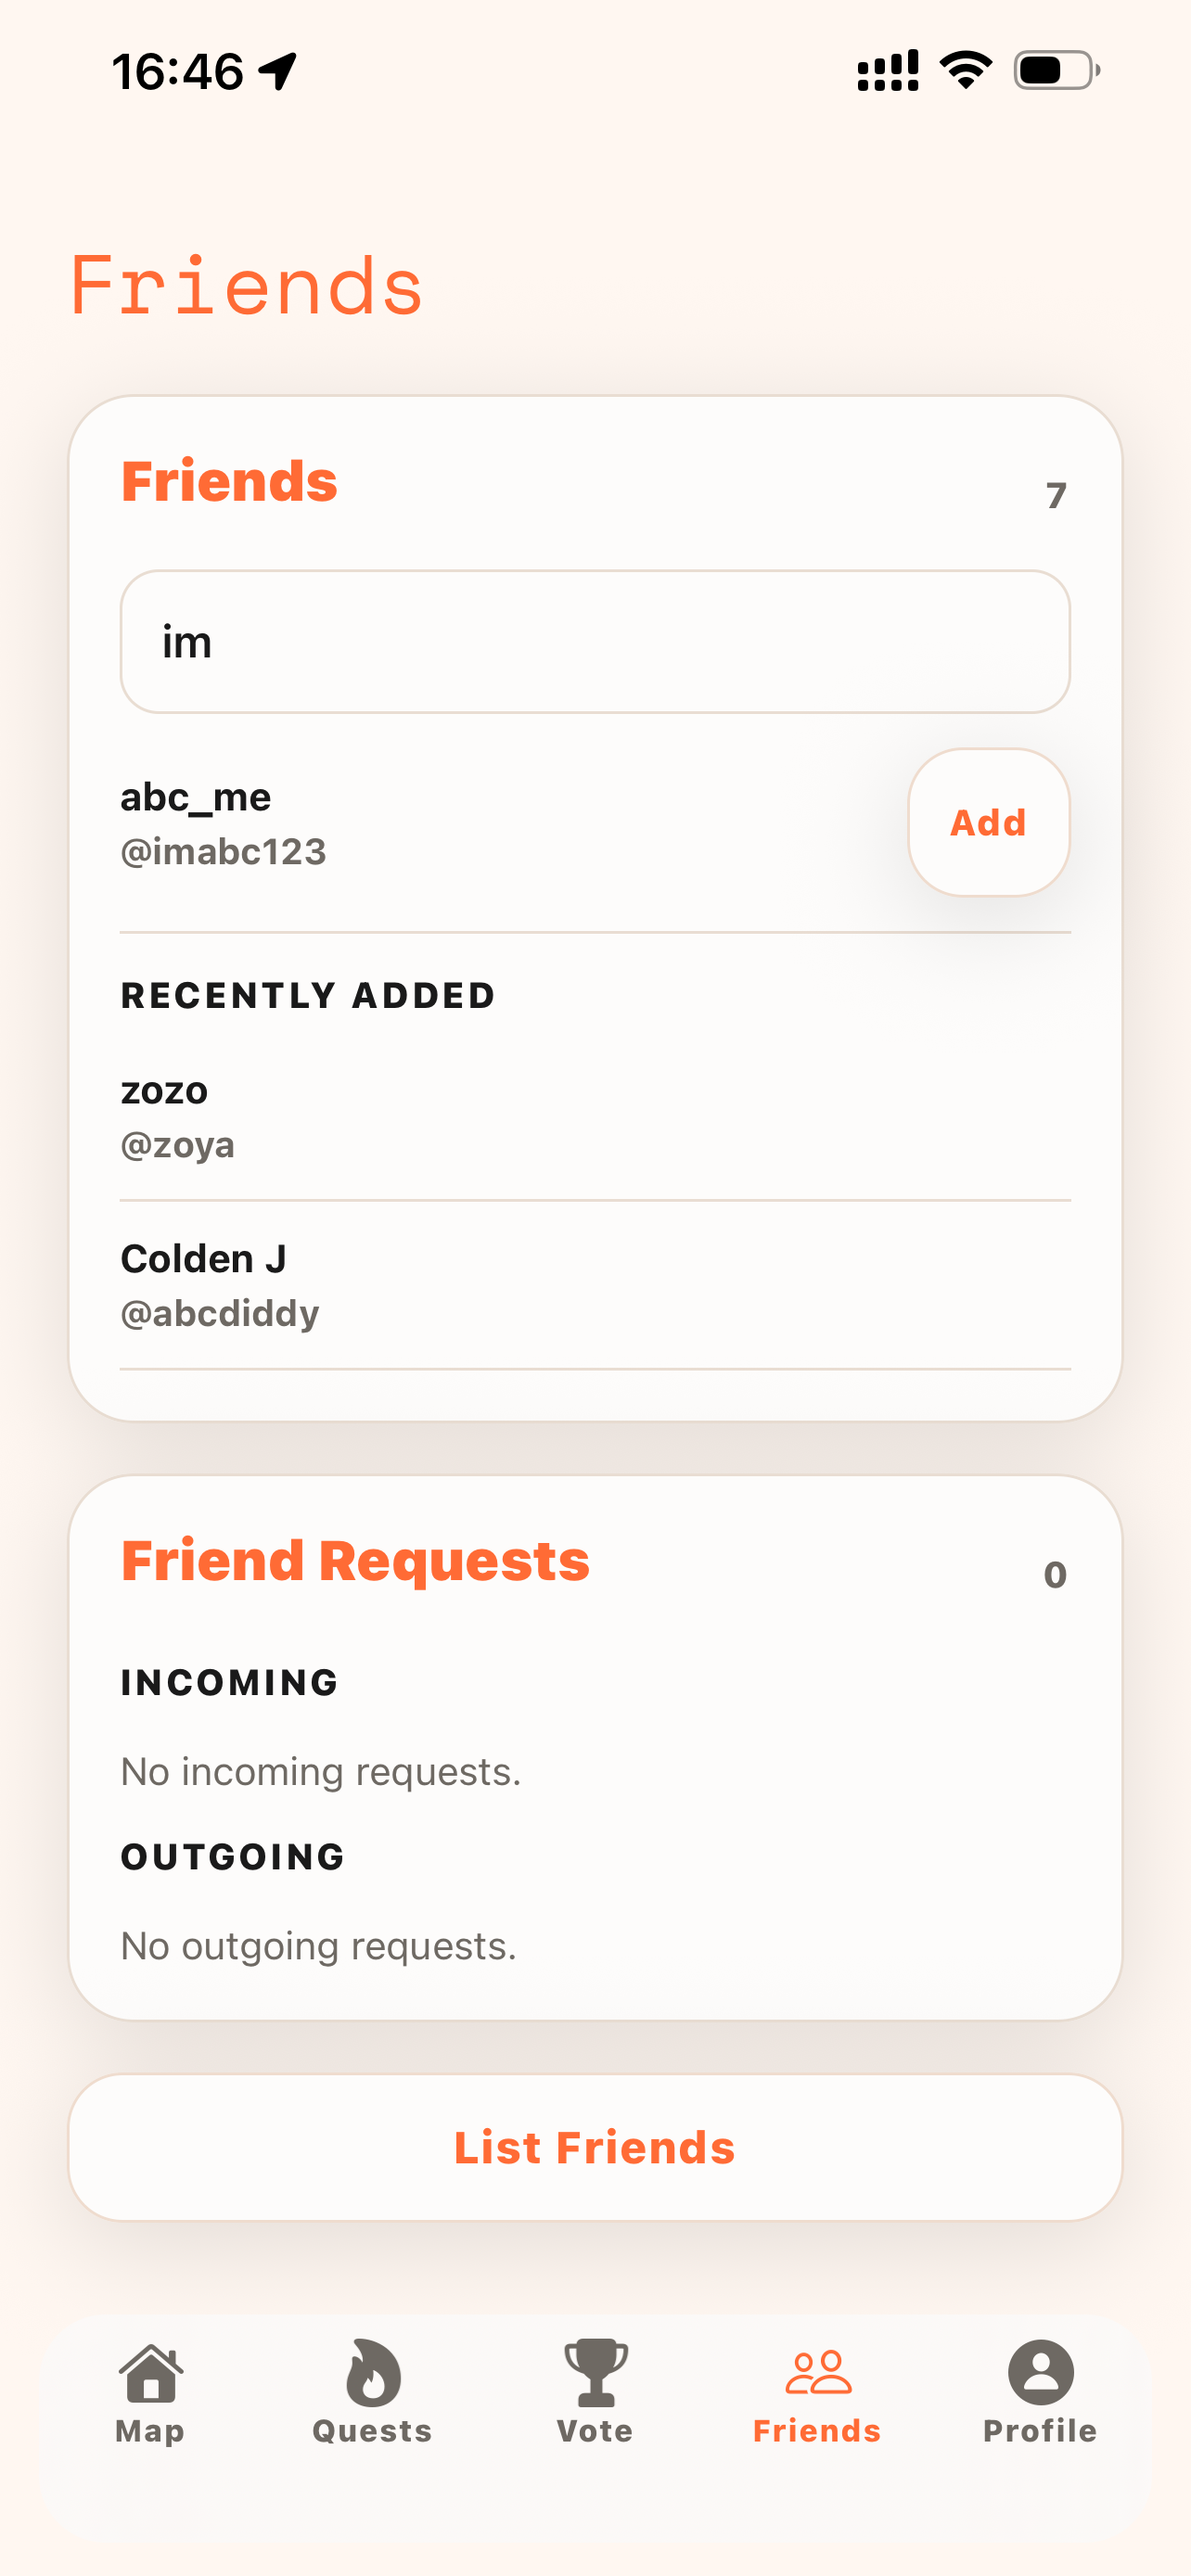
\includegraphics[width=\linewidth]{AppPhotos/Sidequest_Friends.PNG}
    \caption{Friends system UI. \textit{(Social graph and friend challenge interactions.)}}
    \label{fig:appphotos-friends}
  \end{minipage}
\end{figure}

\begin{figure}[!htbp]
  \centering
  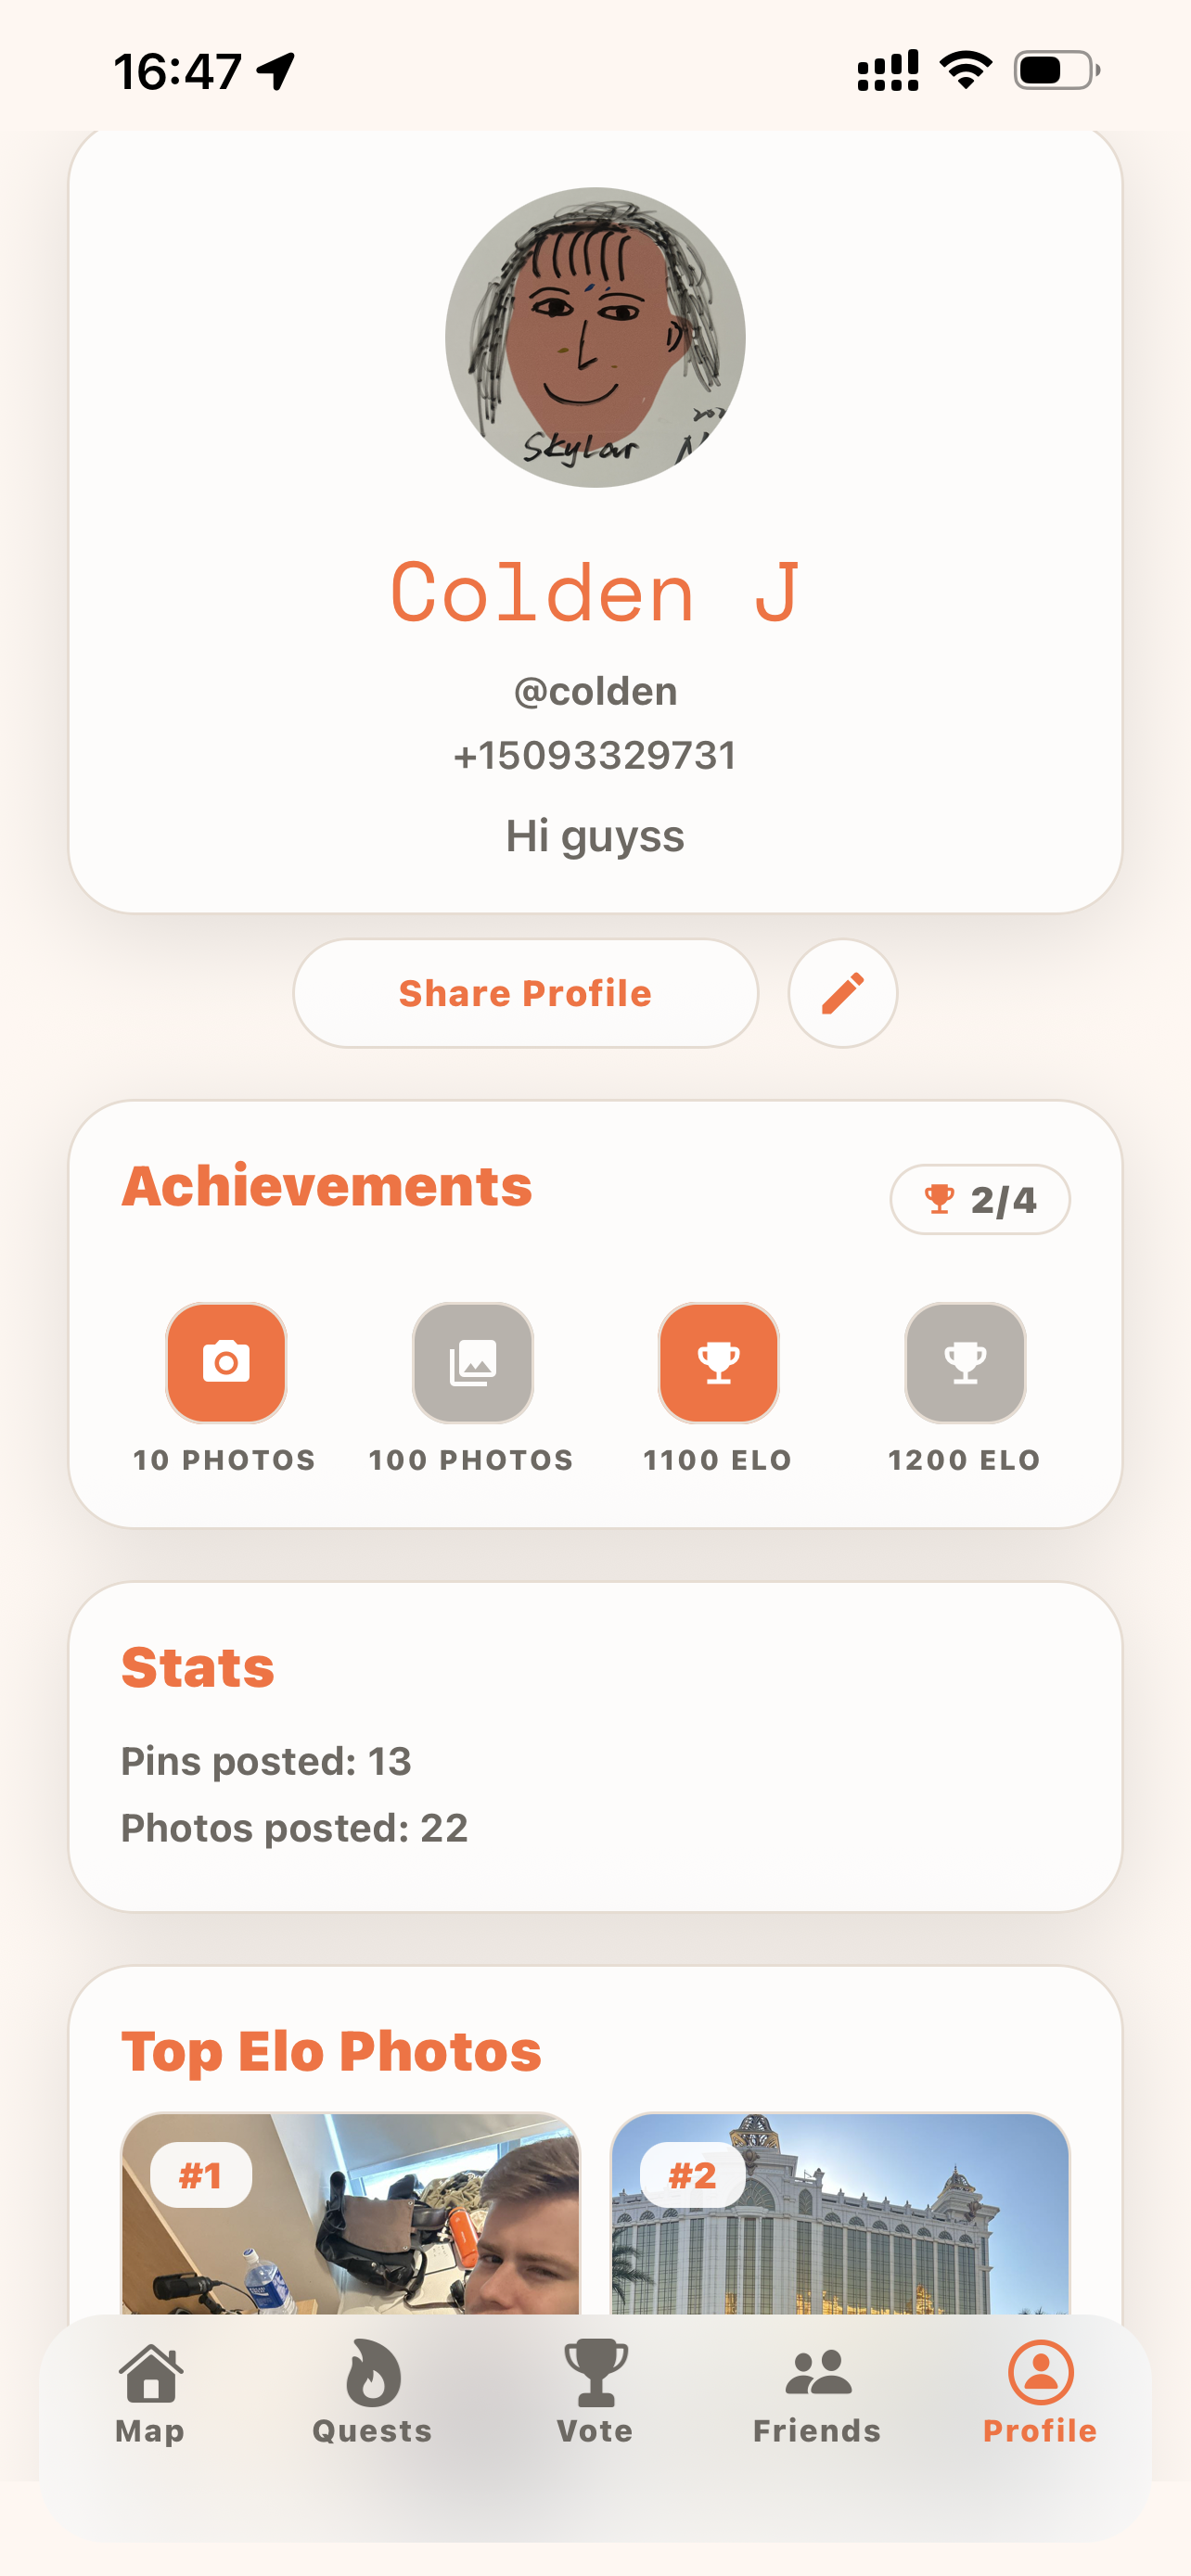
\includegraphics[width=0.48\linewidth]{AppPhotos/Sidequest_Profile.PNG}
  \caption{Profile view. \textit{(User profile page with identity and participation details.)}}
  \label{fig:appphotos-profile}
\end{figure}

\section*{REFERENCES}

{\setlength{\parindent}{0pt}%
\setlength{\parskip}{0.6\baselineskip}%
\newcommand{\mlaentry}[1]{\noindent\hangindent=0.5in\hangafter=1 #1\par}%
\mlaentry{Abidin, Crystal. “Visibility Labour: Engaging with Influencers’ Fashion Brands and \#OOTD Advertorial Campaigns on Instagram.” \textit{Media International Australia}, vol. 161, no. 1, 2016, pp. 86--100. https://doi.org/10.1177/1329878X16665177.}
\mlaentry{BeReal. “BeReal: Your Friends for Real.” BeReal, https://bere.al.}
\mlaentry{Biskjaer, Michael Mose, Peter Dalsgaard, and Kim Halskov. “A Constraint-Based Understanding of Design Spaces.” \textit{Proceedings of the SIGCHI Conference on Human Factors in Computing Systems}, 2014, pp. 2599--2608. https://doi.org/10.1145/2556288.2557342.}
\mlaentry{Bucher, Taina. “Want to Be on the Top? Algorithmic Power and the Threat of Invisibility on Facebook.” \textit{New Media \& Society}, vol. 14, no. 7, 2012, pp. 1164--1180. https://doi.org/10.1177/1461444812440159.}
\mlaentry{de Souza e Silva, Adriana, and Daniel M. Sutko. \textit{Digital Cityscapes: Merging Digital and Urban Playspaces}. Peter Lang, 2009.}
\mlaentry{Deterding, Sebastian, et al. “From Game Design Elements to Gamefulness: Defining ‘Gamification.’” \textit{Proceedings of the 15th International Academic MindTrek Conference}, 2011, pp. 9--15. https://doi.org/10.1145/2181037.2181040.}
\mlaentry{Hemment, Drew. “Locative Arts.” \textit{Leonardo}, vol. 39, no. 4, 2006, pp. 348--355. https://doi.org/10.1162/leon.2006.39.4.348.}
\mlaentry{Instagram. “About Instagram.” Instagram, https://about.instagram.com.}
\mlaentry{Niantic, Inc. “Pokémon GO.” Niantic, 2016, https://pokemongolive.com.}
\mlaentry{Nielsen, Jakob. \textit{Usability Engineering}. Morgan Kaufmann, 1994.}
\mlaentry{Norman, Don. \textit{The Design of Everyday Things}. Revised and expanded ed., Basic Books, 2013.}
\mlaentry{Snap Inc. “Snapchat.” Snap, https://snap.com.}
\mlaentry{Stokes, Patricia D. \textit{Creativity from Constraints: The Psychology of Breakthrough}. Springer, 2005.}
\mlaentry{Zimmerman, John, Jodi Forlizzi, and Shelley Evenson. “Research through Design as a Method for Interaction Design Research in HCI.” \textit{Proceedings of the SIGCHI Conference on Human Factors in Computing Systems}, 2007, pp. 493--502. https://doi.org/10.1145/1240624.1240704.}
}

\end{document}

\begin{figure}[!htbp]
  \centering
  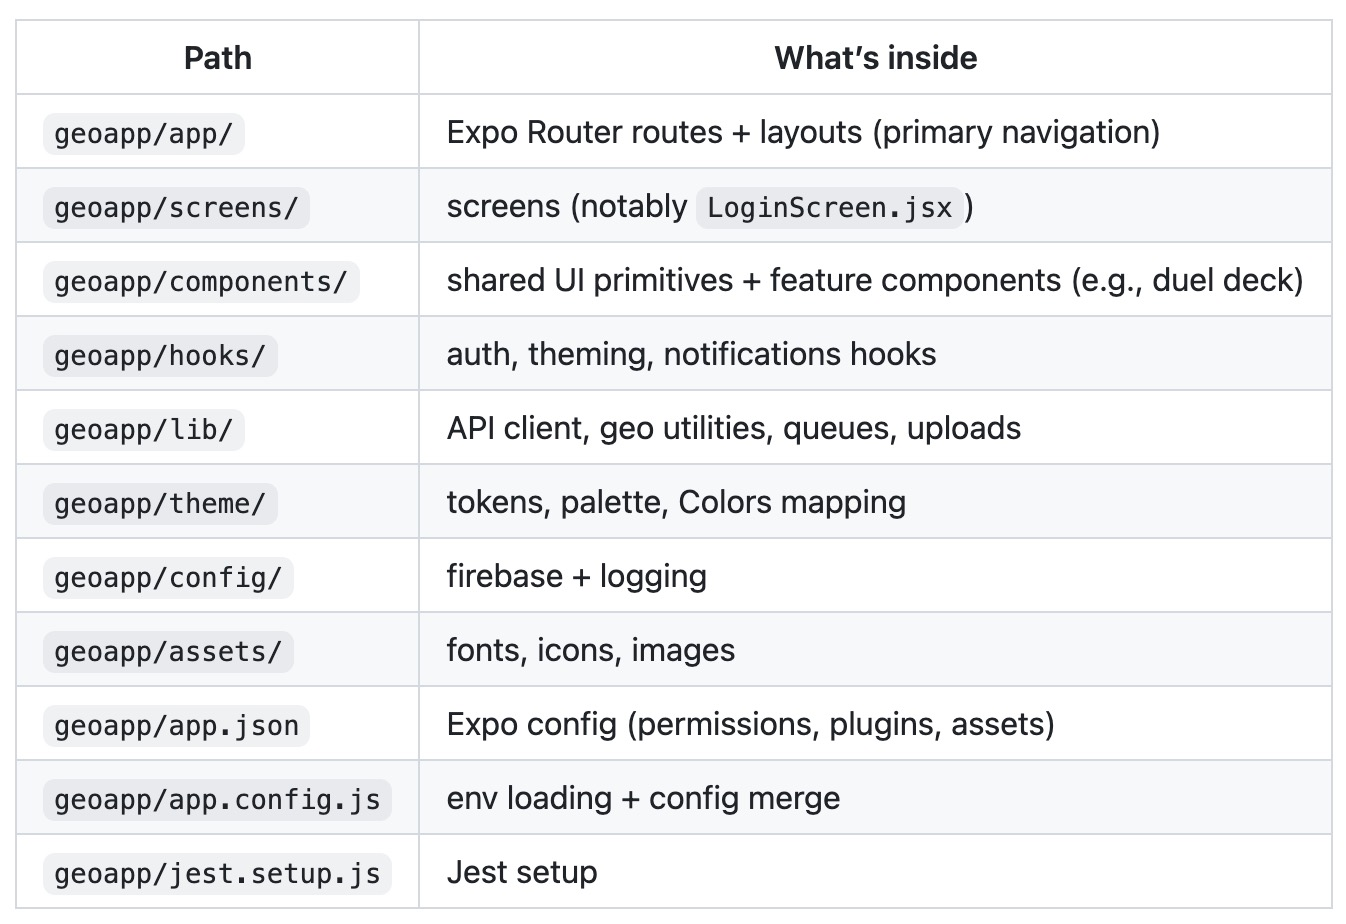
\includegraphics[width=0.7\linewidth]{FrontendStructureChart.jpg}
  \caption{Frontend structure chart. \textit{(High-level organization of the React Native app.)}}
  \label{fig:frontend-structure}
\end{figure}

\subsection*{2. Backend: Node.js with Express (MERN)}

The backend is built using Node.js and Express, forming part of the MERN (MongoDB, Express, React, Node) stack.

Node.js allows JavaScript to run server-side. Using the same language across frontend and backend reduces context switching and improves development speed. Express is a REST API layer that is simple, flexible, and widely adopted.

The primary advantage of this stack is cohesion. React on the frontend and Node/Express on the backend share conceptual patterns (components, middleware, JSON APIs). This makes it easy to reason about how data flows across the system.

Alternative backend frameworks were considered. Python (Flask or Django) would provide strong tooling and readability. Additionally, I have significant prior experience with both Python and Flask, and thus am much more comfortable with this type of backend. However, the flexibility and ecosystem alignment of Express made it better suited for rapid iteration and a custom-designed API. A more rigid framework would increase complexity, something against our design philosophy.

The backend enforces server-authoritative logic. All ranking updates (Elo calculations), vote validation, and rate limiting occur server-side. This prevents manipulation from the client and preserves competitive integrity.

\subsection*{3. Data Architecture and Authentication}

\subsubsection*{3.1 Database: MongoDB Atlas + Mongoose}

SideQuest uses MongoDB Atlas as its primary database. MongoDB is a document-oriented database, meaning it stores JSON-like documents rather than strictly relational tables. This allows for flexible schema evolution, which was valuable during early development when data models changed frequently.

MongoDB was selected partially due to its generous free tier and ease of cloud deployment. Atlas provides managed hosting, backups, and scaling without requiring infrastructure management.

However, MongoDB is not relational in the traditional SQL sense. To introduce structure and validation, Mongoose is used as an Object Data Modeling (ODM) layer. Mongoose defines schemas, enforces validation rules, and creates relationships between collections. While MongoDB itself does not enforce foreign key constraints, Mongoose allows us to simulate relational structure through references and schema design.

A relational SQL database (ex: PostgreSQL) was considered. SQL databases provide stronger built-in relational guarantees and transactional consistency. However, SideQuest data shape is naturally hierarchical and document shaped, not deeply relational. For example, a given pin is usually fetched as a nested JSON in the API response regardless: thus, the symmetry feels both natural and convenient. Additionally, MongoDB has a faster iteration model, and lets us evolve documents without migrations. With Postgress, schema migrations would be required each time we changed data models, which has been troublesome on past projects. For a rapidly changing product, schema rigidity can slow development.

\subsubsection*{3.2 Media Storage: Firebase Storage}

Images are not stored directly in MongoDB. Instead, image files are uploaded to Firebase Storage, and only their URIs are stored in the database.

Storing images directly inside MongoDB (for example, as binary blobs) would dramatically increase database size and degrade performance. Databases are optimized for structured data, not large media objects. Separating media storage from structured data is standard practice in production systems. Firebase Storage provides scalable object storage optimized for large files. This separation keeps the database efficient and independent.

\subsubsection*{3.3 Authentication: Firebase Auth}

Authentication is handled using Firebase Authentication. Users can sign in via email/password, phone (SMS), or Google accounts.

Implementing authentication from scratch would require handling password hashing, token management, SMS verification infrastructure, and security auditing. Firebase abstracts this complexity while still allowing server-side token verification using Firebase Admin SDK.

All privileged backend routes verify Firebase-issued ID tokens before allowing writes. This ensures that authentication is also enforced server-side, securing server routes.

\subsection*{4. Deployment, Containerization, and Testing}

The backend is containerized using Docker. Containerization ensures the application runs identically across development and production environments. Dependencies, Node versions, and environment variables are packaged consistently. A common developer joke captures the problem Docker is meant to solve: a developer's code works locally, but upon pushing to someone else's computer (or prod), it immediately breaks. The developer simply responds, "It works on my machine", and proceeds to ignore the problem, much to the distress of everyone else on the team. Docker is intended to eliminate this problem, by standardizing the execution environment.

The Docker container is deployed to Google Cloud Run. Cloud Run automatically scales instances based on traffic and provides global accessibility without managing servers manually. Compared to traditional VM hosting, Cloud Run abstracts infrastructure management while still allowing full control over the runtime env.

Alternative deployment options included Heroku or traditional virtual machines. However, Docker + Cloud Run provided greater control and scalability without excessive complexity. Additionally, the CI/CD pipeline was incredibly easy to set up, and the service is generally very straightforward to work with.

For API validation and debugging, Postman is used to test endpoints independently of the frontend. This allows for isolating backend issues without UI interference. Jest is used for unit testing critical backend logic.

\subsection*{5. User Testing and Iterative Validation}

SideQuest’s architecture decisions are heavily driven by user feedback and TestFlight deployment.

\subsubsection*{5.1 TestFlight as Formal Evaluation Channel}

TestFlight builds were released in rapid cycles. Each release included observed task flows, post-session qualitative feedback, and bug reproduction attempts. This method allows for controlled evaluation of user UX smoothness, upload reliability, and issue detection.

\subsubsection*{5.2 Selected User Feedback and Responses}

The documented user feedback revealed abundant major issue categories. We noted qualitative feedback both on a 'product backlog' whiteboard \textit{(Fig.~\ref{fig:user-feedback-wall})}, as well as in a shared Obsidian notes app.

\begin{figure}[!htbp]
  \centering
  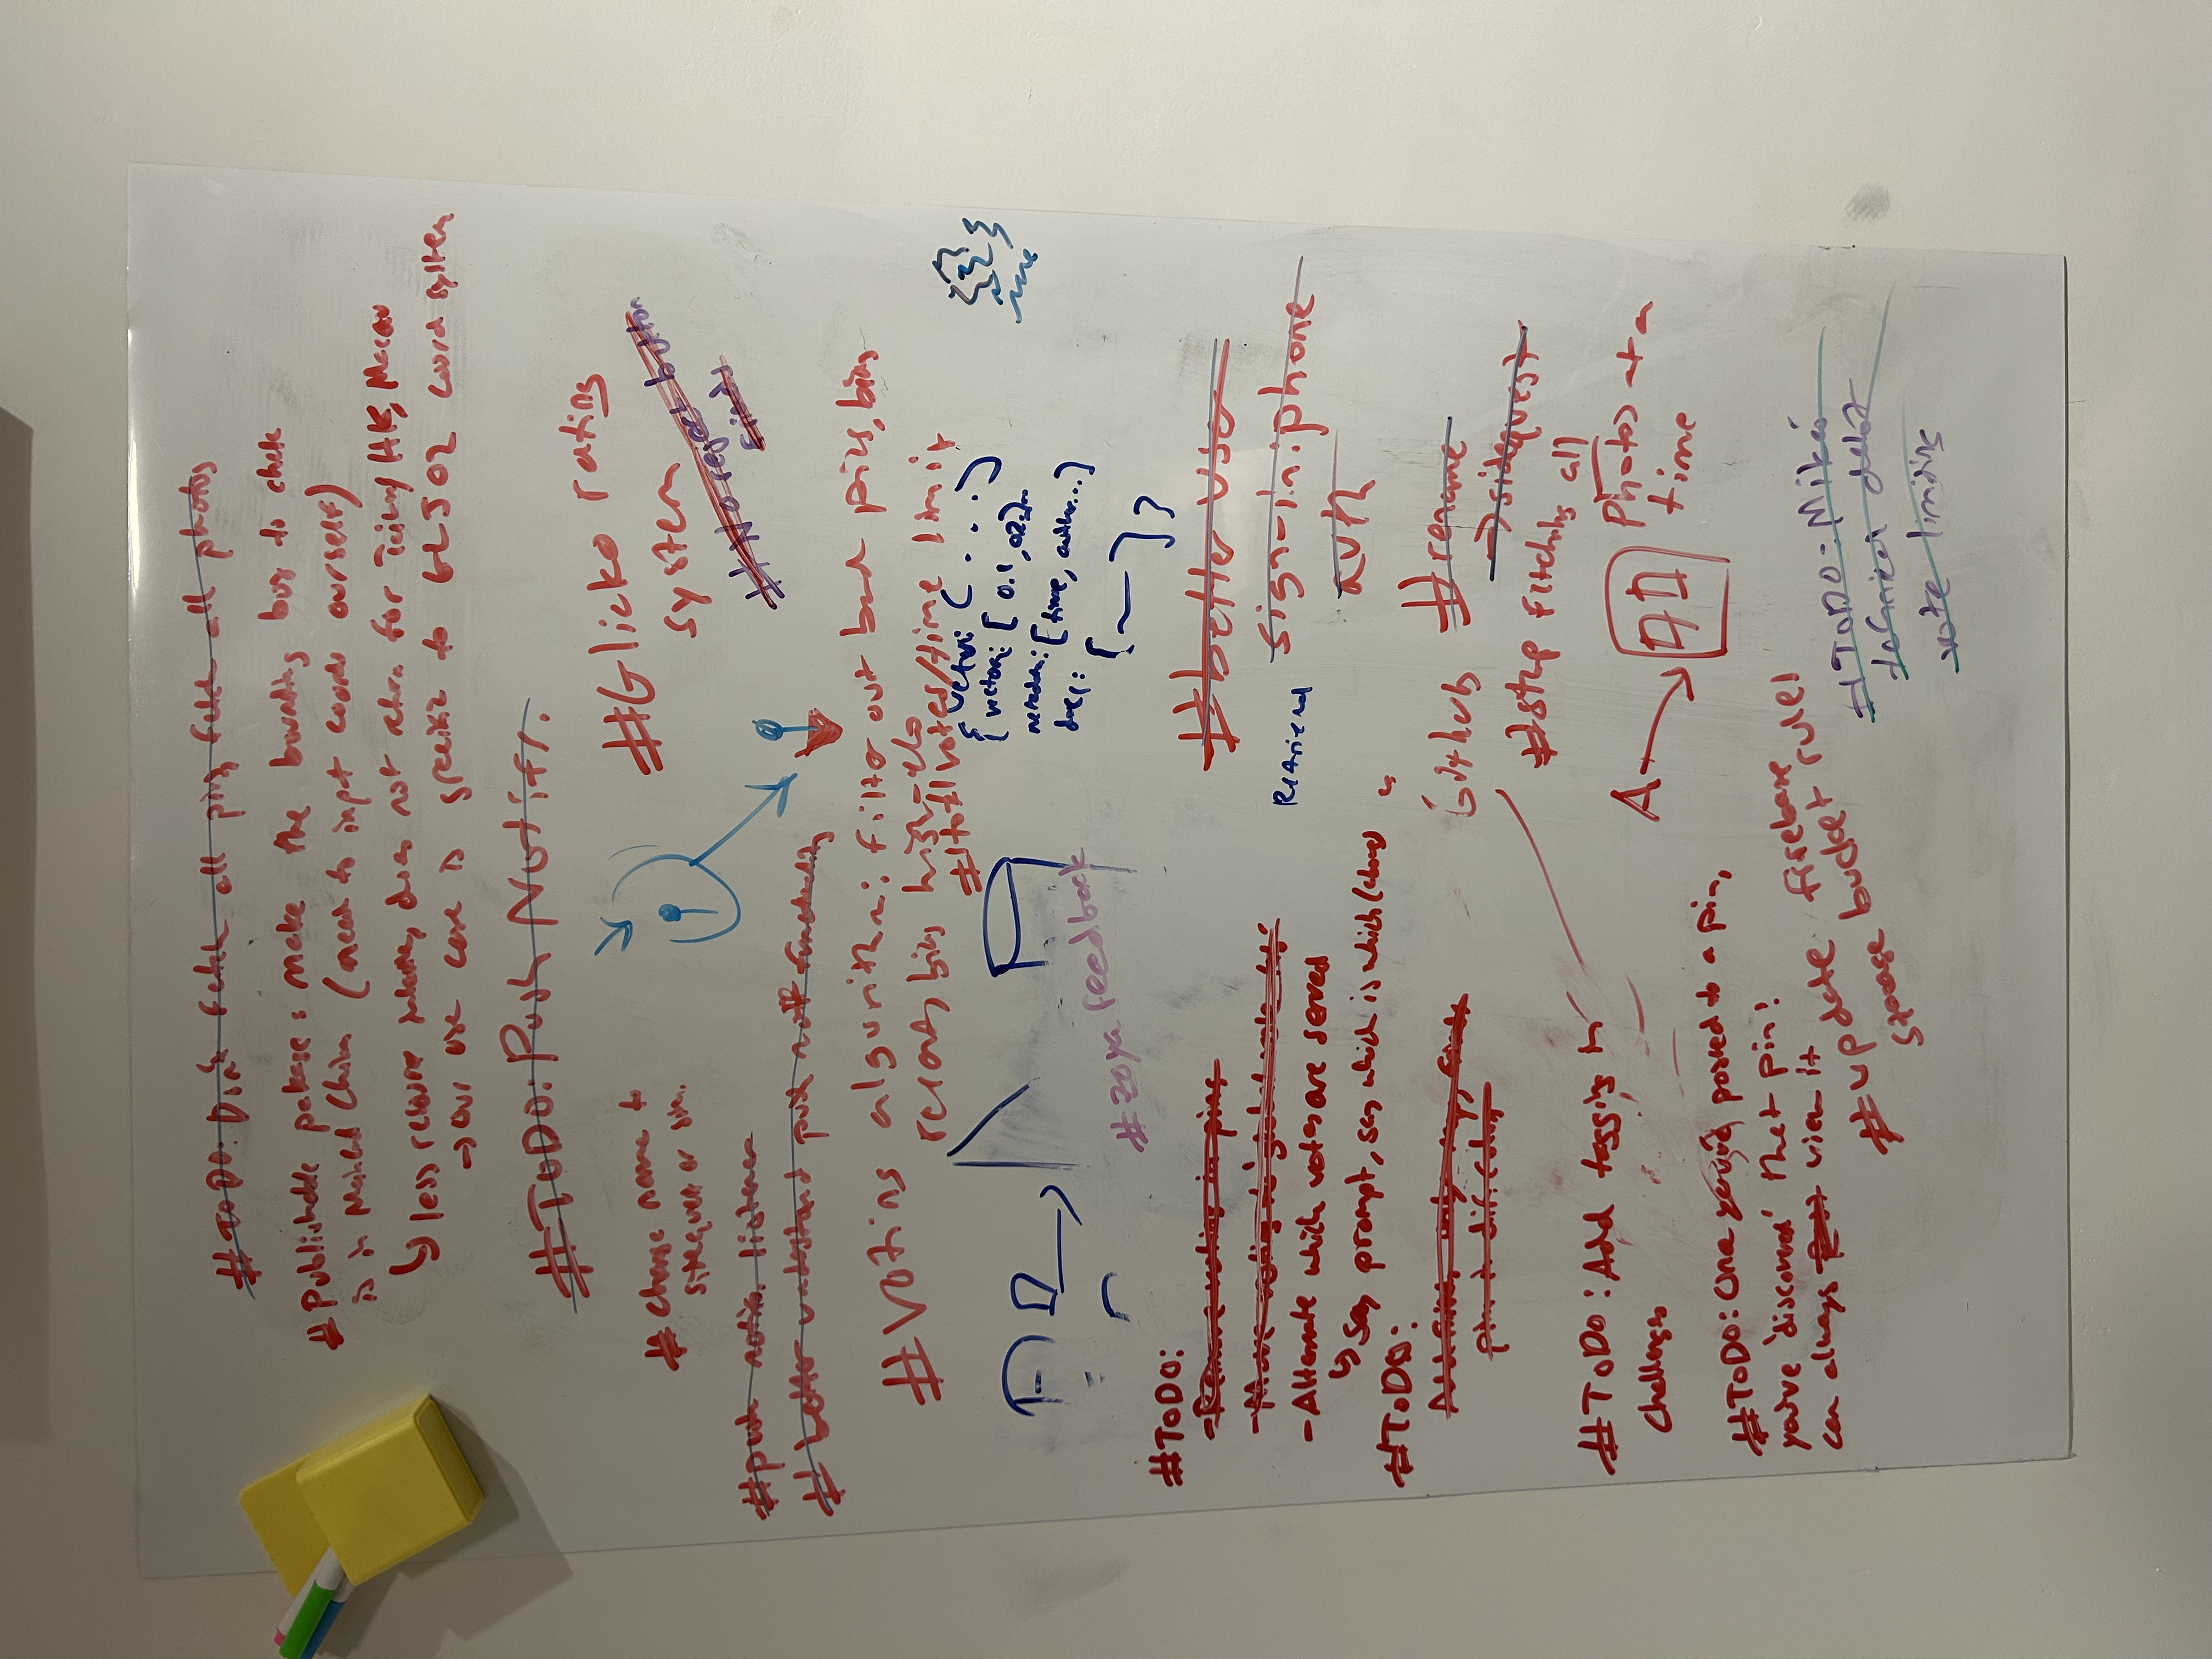
\includegraphics[width=0.4\linewidth, angle=-90]{UserFeedbackWall.jpeg}
  \caption{User feedback wall / product backlog snapshot. \textit{(Whiteboard backlog used to track open issues.)}}
  \label{fig:user-feedback-wall}
\end{figure}

\renewcommand{\arraystretch}{1.25}
\begin{center}
\begin{tabular}{|p{0.32\linewidth}|p{0.62\linewidth}|}
\hline
\textbf{Identified problem} & \textbf{Resolution} \\
\hline
Swipe voting confusion: flicker during swipes. & DuelDeck animation logic decoupled from vote submission timing; image prefetching introduced; hard locks on gestures removed to make UI more responsive. \\
\hline
Upload reliability issues: repeated presses needed; unclear upload state. & Explicit upload state management; promise resolution tracking; UI toast (notification message) on success; guards to prevent duplicate submissions. \\
\hline
Aesthetic issues: poor cohesiveness. & Centralized token system (spacing, radii, typography); unified palette implementation; shared component primitives; removal of ad-hoc inline styles; still being improved. \\
\hline
Elo integrity: ranking manipulation. & Server-side vote validation; token-based duel confirmation; rate limits and hourly caps. \\
\hline
\end{tabular}
\end{center}

\subsection*{6. Design Methods }

As we have already talked extensively about theory, this section aims to discuss specific process innovations.

\subsubsection*{3.1 Production Prototyping}

Instead of designing visuals first and engineering later, SideQuest follows a 'capability-first' method. Roughly, this means that system functionality is built out first (backend), and UI is designed around these system constraints. This allows for:

Simple UI iteration with confidence

Catching concurrency bugs early

\subsubsection*{3.2 Git-Based Dev }

Git is simply incredible, and deserves an honorable mention. Git was used for version control and structured iteration.

Minimal-diff commits were important for identifying isolated behavior changes. One example of this is when fixing a particularly nasty UI bug related to issues only on every 3rd served photo, it was necessary to revert commits back several weeks to localize when the problem originated. Only by reverting to an earlier version was the problem identified and solved. Commit history also serves as a repository of product evolution and architectural maturation \textit{(Fig.~\ref{fig:repo-commit-diagram})}.

\begin{figure}[!htbp]
  \centering
  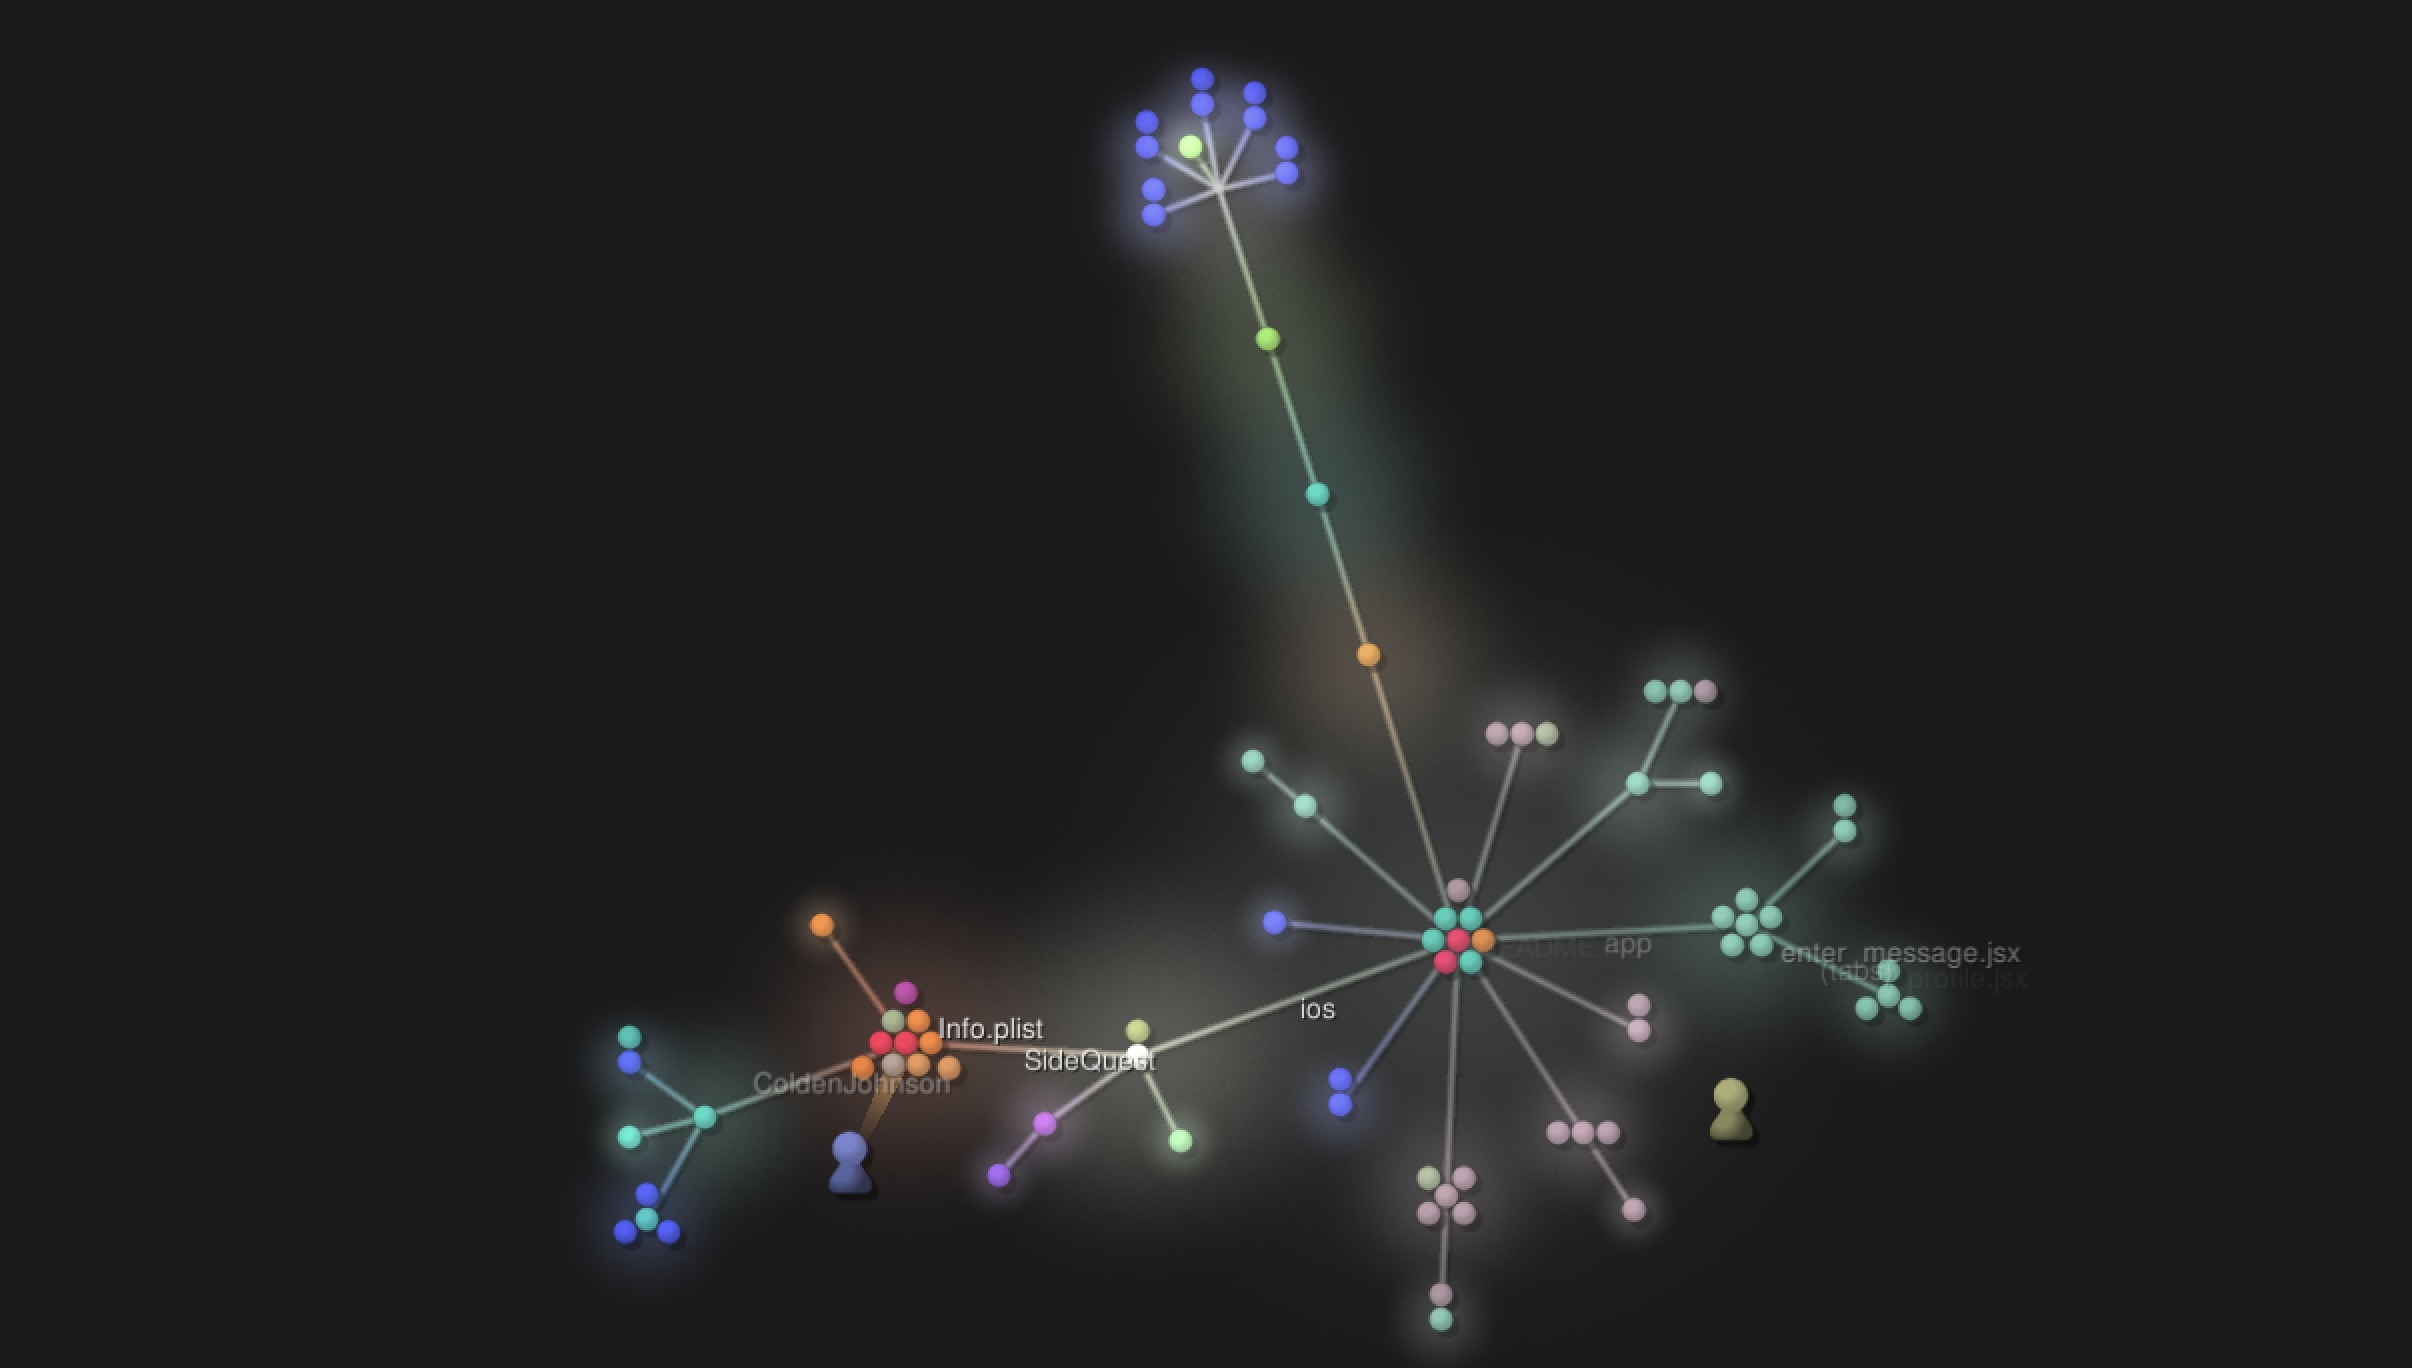
\includegraphics[width=0.9\linewidth]{RepoCommitDiagram.jpg}
  \caption{Gource Git commit visualization with multiple contributors and versioning.}
  \label{fig:repo-commit-diagram}
\end{figure}

\subsubsection*{3.3 Agile Development }

Development prioritized constant iterative improvement based on user feedback, following the Agile development philosophy. Each cycle began with a TestFlight release, followed by direct observation of user interaction.

As issues emerged, we revisited architectural components in real time. It was important to have little emotional attachment to the current state of the project, and readily refactor when necessary. In several cases, this resulted in major overhauls of the app. After implementing changes, a new build was released and the cycle repeated. Over time, this iterative pattern functions like gradient descent optimization, as iterative releases gradually move the user toward a smoother product experience.

This process assumes that all of our assumptions are incorrect. Design and architecture remains highly fluid.

\subsection*{7. AI Usage In Modern Development }

AI usage in modern app development could be an entire paper on its own. That said, we think it is instructive to talk briefly about the ways we're using AI in our workflows and how it assists with architectural judgement.

We use primarily Codex 5.3 for simple implementation-related coding tasks. Architectural decisions are typically informed using a mix of Claude and ChatGPT (along with docs/example GitHubs). This separation is relatively strict, as models perform best when given well-scoped problems. In our workflow, we have found that spending the majority of time upfront thinking about architecture results in far easier implementation later on.

We maintain an extensive custom prompt and model library for recurring tasks. For example, our `summary' task is adapted from a leaked Claude Code system summary template, and is used to prevent context overload during extended terminal sessions. Context management more broadly is critical. To address this, we use a combination of MCP servers for scoped context exposure, deep research for highly complex decisions, and manual identification of relevant documentation and code snippets when pursuing specific directions. In addition, we run several custom model configurations within a local Open WebUI instance connected to OpenRouter \textit{(see Fig.~\ref{fig:openwebui-example})}. These custom models allow for targeting specific jobs/recurring problem categories (for example, dealing with Elo/ranking logic or writing README documentation).

In short, AI is an important aspect of modern app development, and we have put a significant amount of energy into setting up appropriate workflows to fully take advantage of this.

\begin{figure}[!htbp]
  \centering
  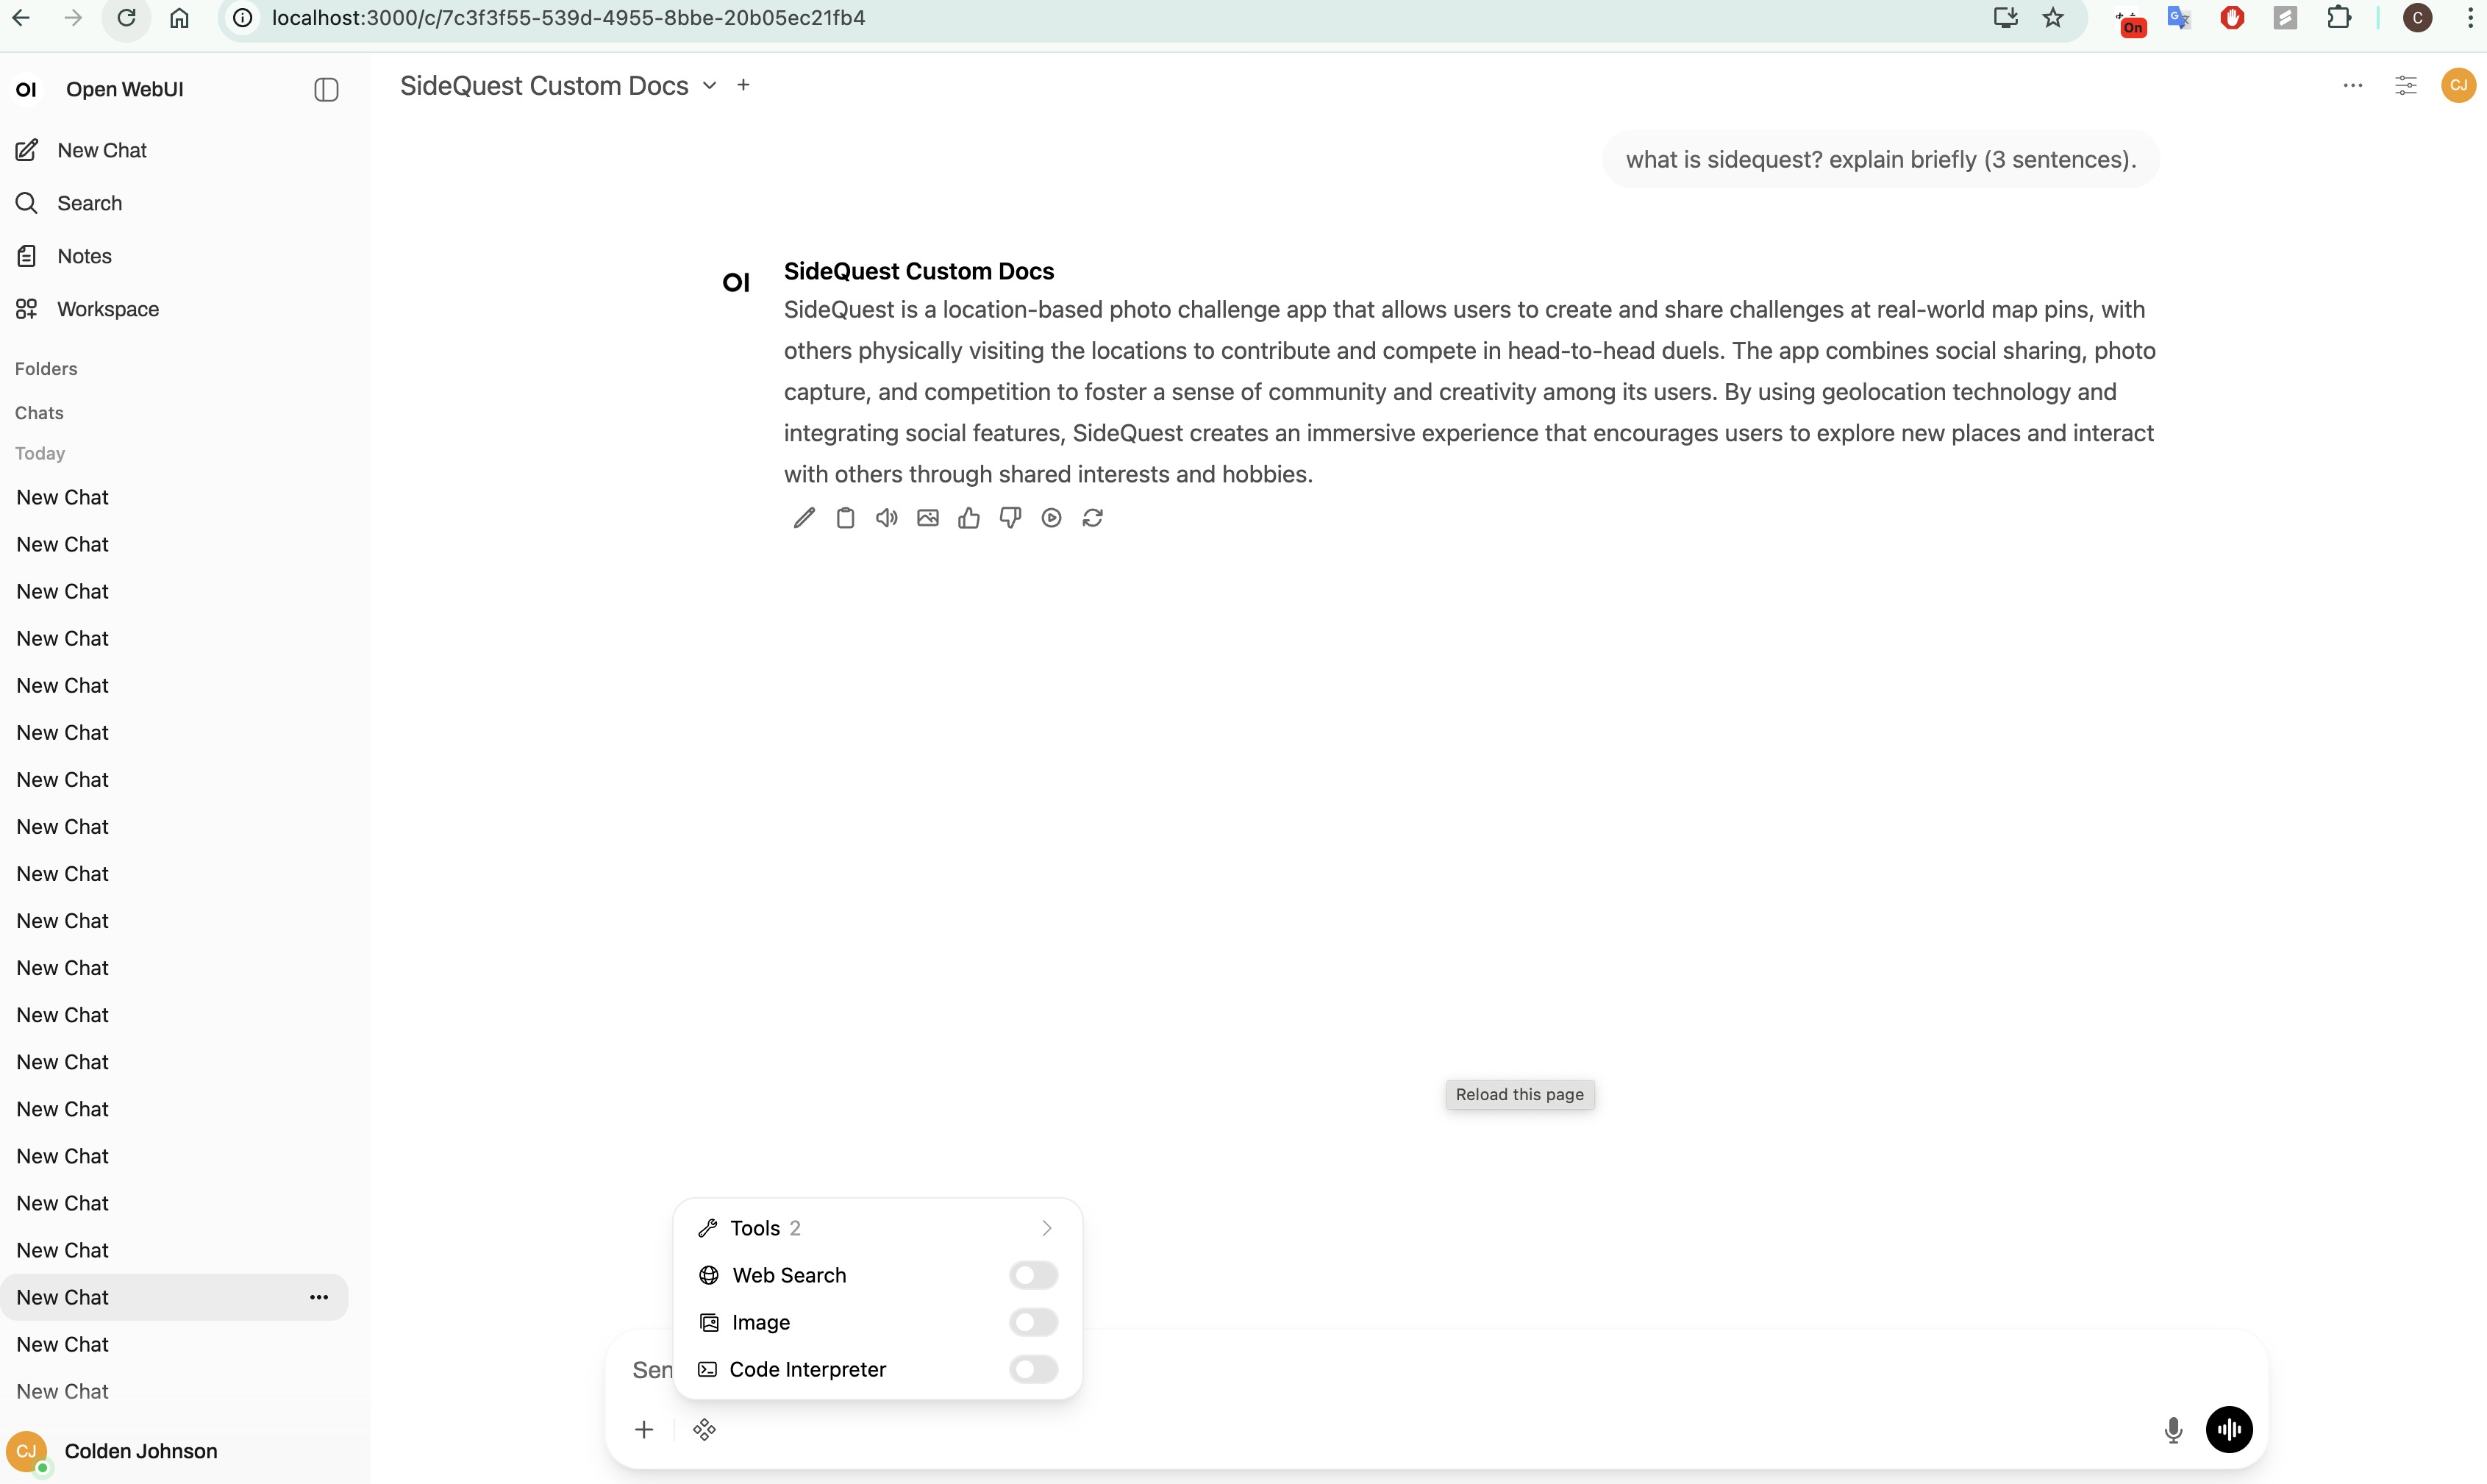
\includegraphics[width=0.5\linewidth]{OpenWebUI_example.jpg}
  \caption{Open WebUI local model workflow. \textit{Example of custom model config used for scoped, recurring docs querying/generation.}}
  \label{fig:openwebui-example}
\end{figure}

% =========================
% FINAL OUTCOME
% =========================
\section*{FINAL OUTCOME}
\subsection*{5.1 Concept statement}
SideQuest is a creative platform that transforms spaces into living, community-built creative artifacts. A user stands somewhere, captures a moment, adds a short prompt, and plants that creative challenge onto a map. Over time, this space becomes a shared public square shaped by many contributors. 

SideQuest is 'the anti-Instagram': while many social platforms reward passive scrolling, SideQuest asks users to explore and create.

Beyond being an innovative concept, SideQuest is a successful example of a full-stack iOS application published to the App Store and supported by production-grade architecture. The system manages authentication, media storage, geospatial correctness, and user interaction. It has X daily active users, providing evidence that the design holds under real usage conditions.

\subsection*{5.2 What is delivered (artifact inventory)}
This project delivers a complete set of artifacts suitable for a creative practice Signature Work:

\textbf{Primary artifact}
\begin{itemize}[leftmargin=*, itemsep=0.25\baselineskip]
  \item SideQuest iOS App
\end{itemize}

\textbf{Supporting artifacts}
\begin{itemize}[leftmargin=*, itemsep=0.25\baselineskip]
  \item Deployed backend (Dockerized API on Google Cloud Run)
  \item GitHub repository (source code, history, documentation)
  \item Design + testing documentation (TestFlight feedback notes; iterative change history)
  \item Evaluation evidence (DAU trend snapshots; usability findings; bug/issue log excerpts)
  \item Screenshots and visual documentation (final UI states for major flows)
  \item Architecture diagrams
\end{itemize}

\subsection*{5.4 Walkthrough of the final user experience}
<TODO: Upload screenshots here>
Let's look at our friend Krishna's user journey:


-onboarding + SMS
- live map screen
- challenge creation and contribution
-voting, viewing, immersion
-competition and motivation (gamification, duels)
-adding friends

\subsection*{5.5 Evidence of impact}
<TODO:  DAUs, Example challenge pin, outcome metrics table>

<TODO: Reflection, Bibliography, Prof. Feedback>

\begin{figure}[!htbp]
  \centering
  \begin{minipage}[t]{0.48\linewidth}
    \centering
    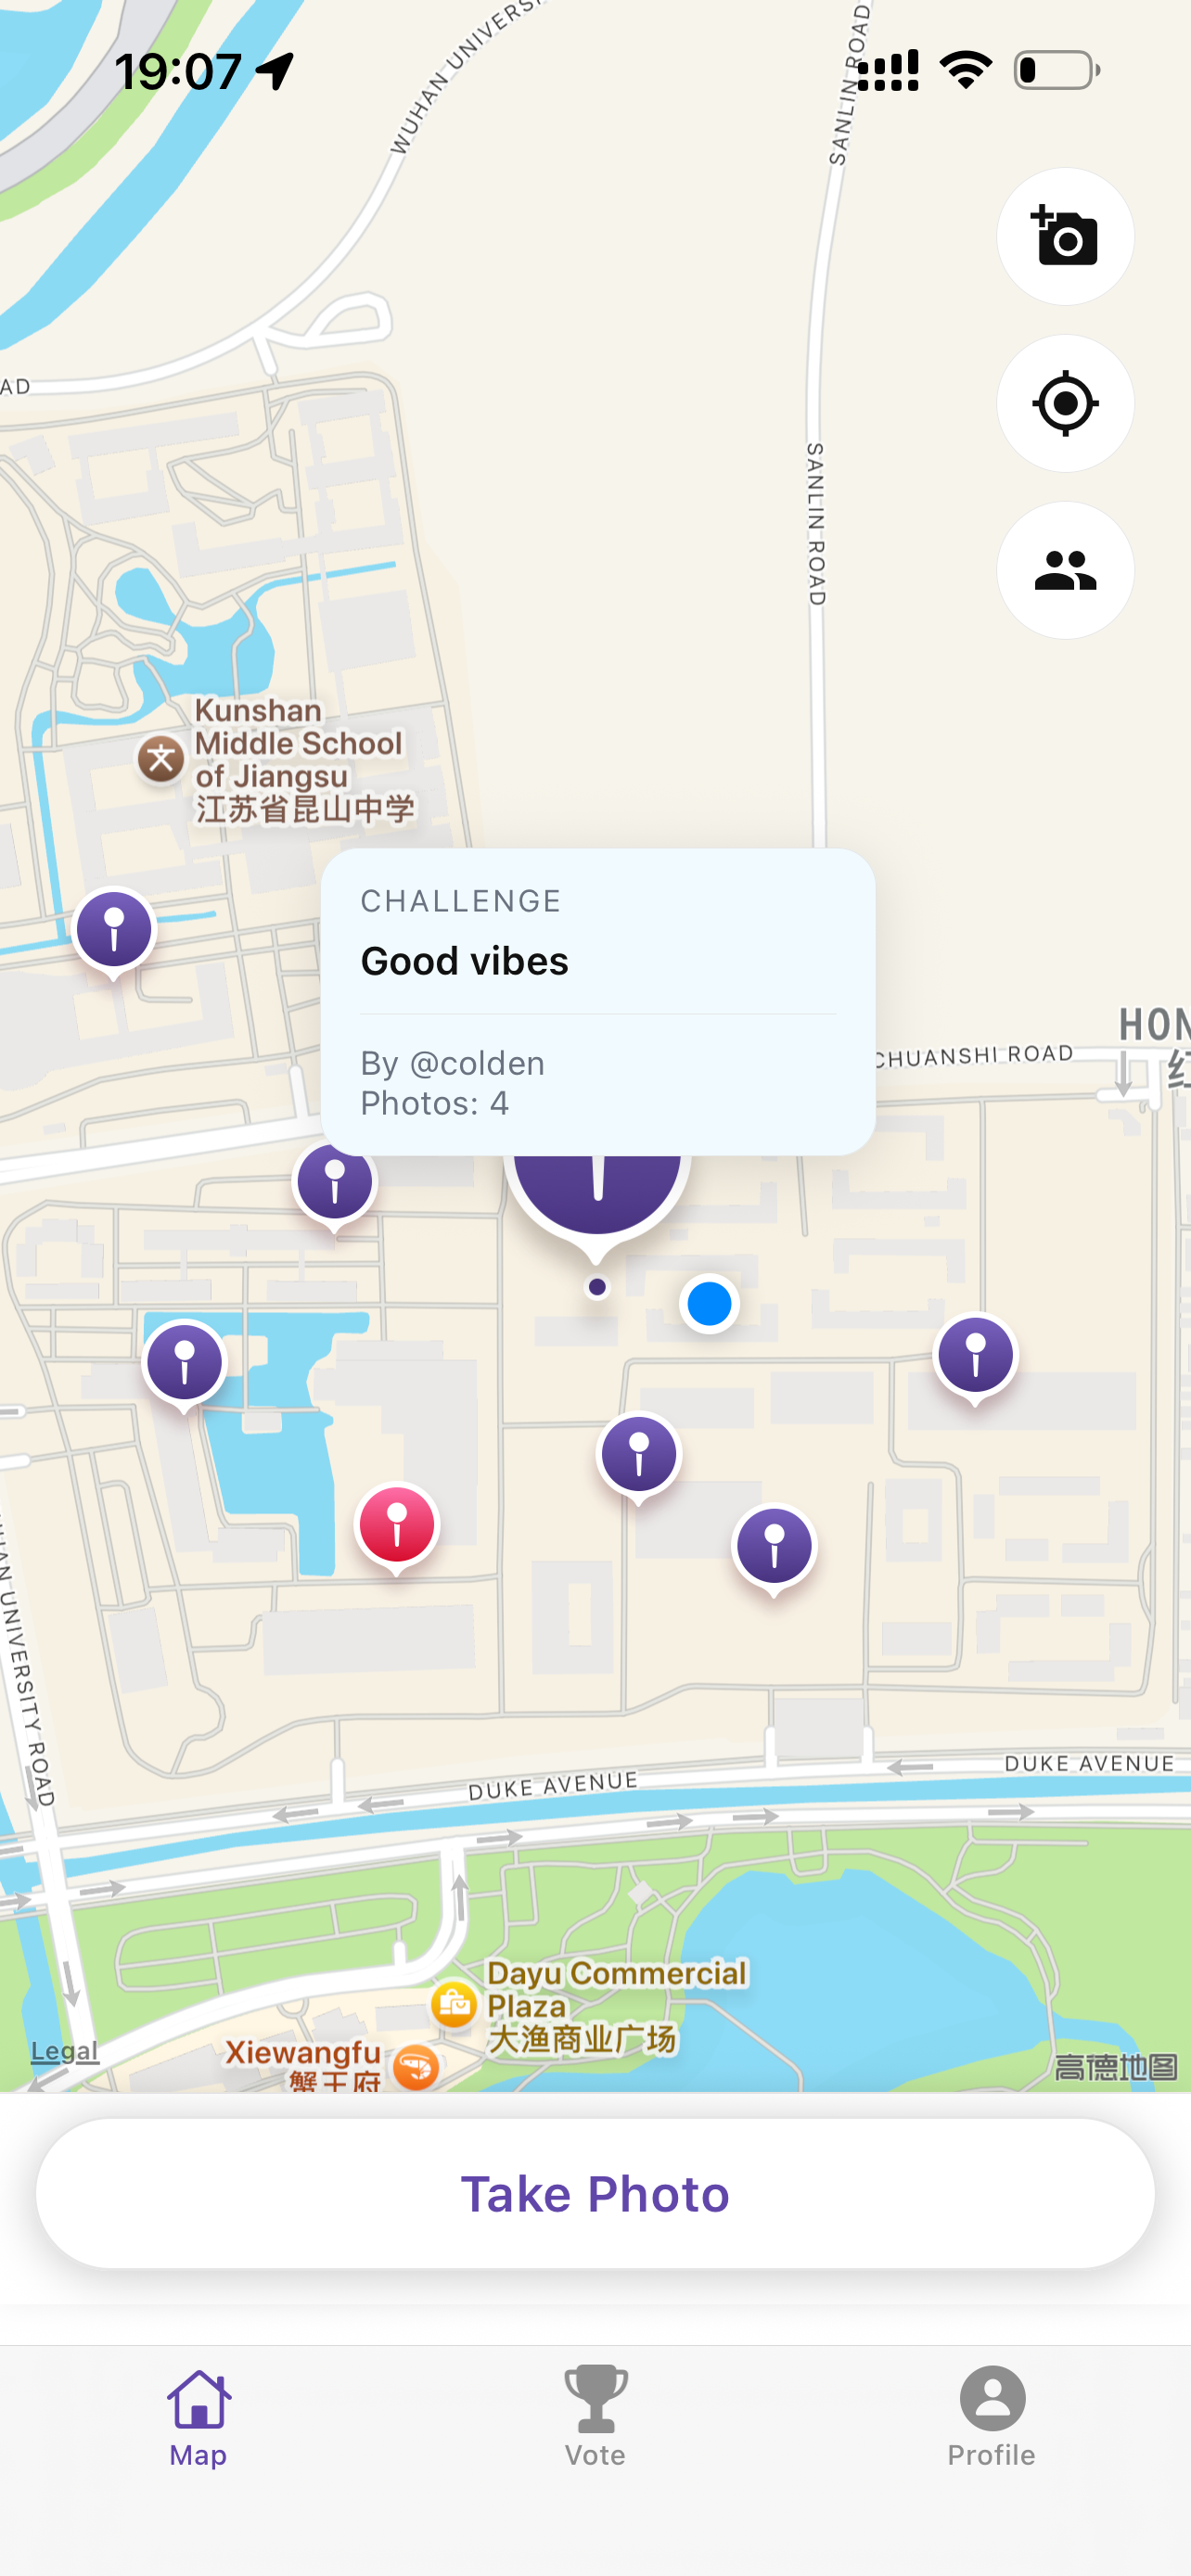
\includegraphics[width=\linewidth]{ChallengeMap.PNG}
    \caption{Challenge map landing page. \textit{(Landing page map view with pin uploads around DKU created by app users.)}}
    \label{fig:challenge-map}
  \end{minipage}\hfill
  \begin{minipage}[t]{0.48\linewidth}
    \centering
    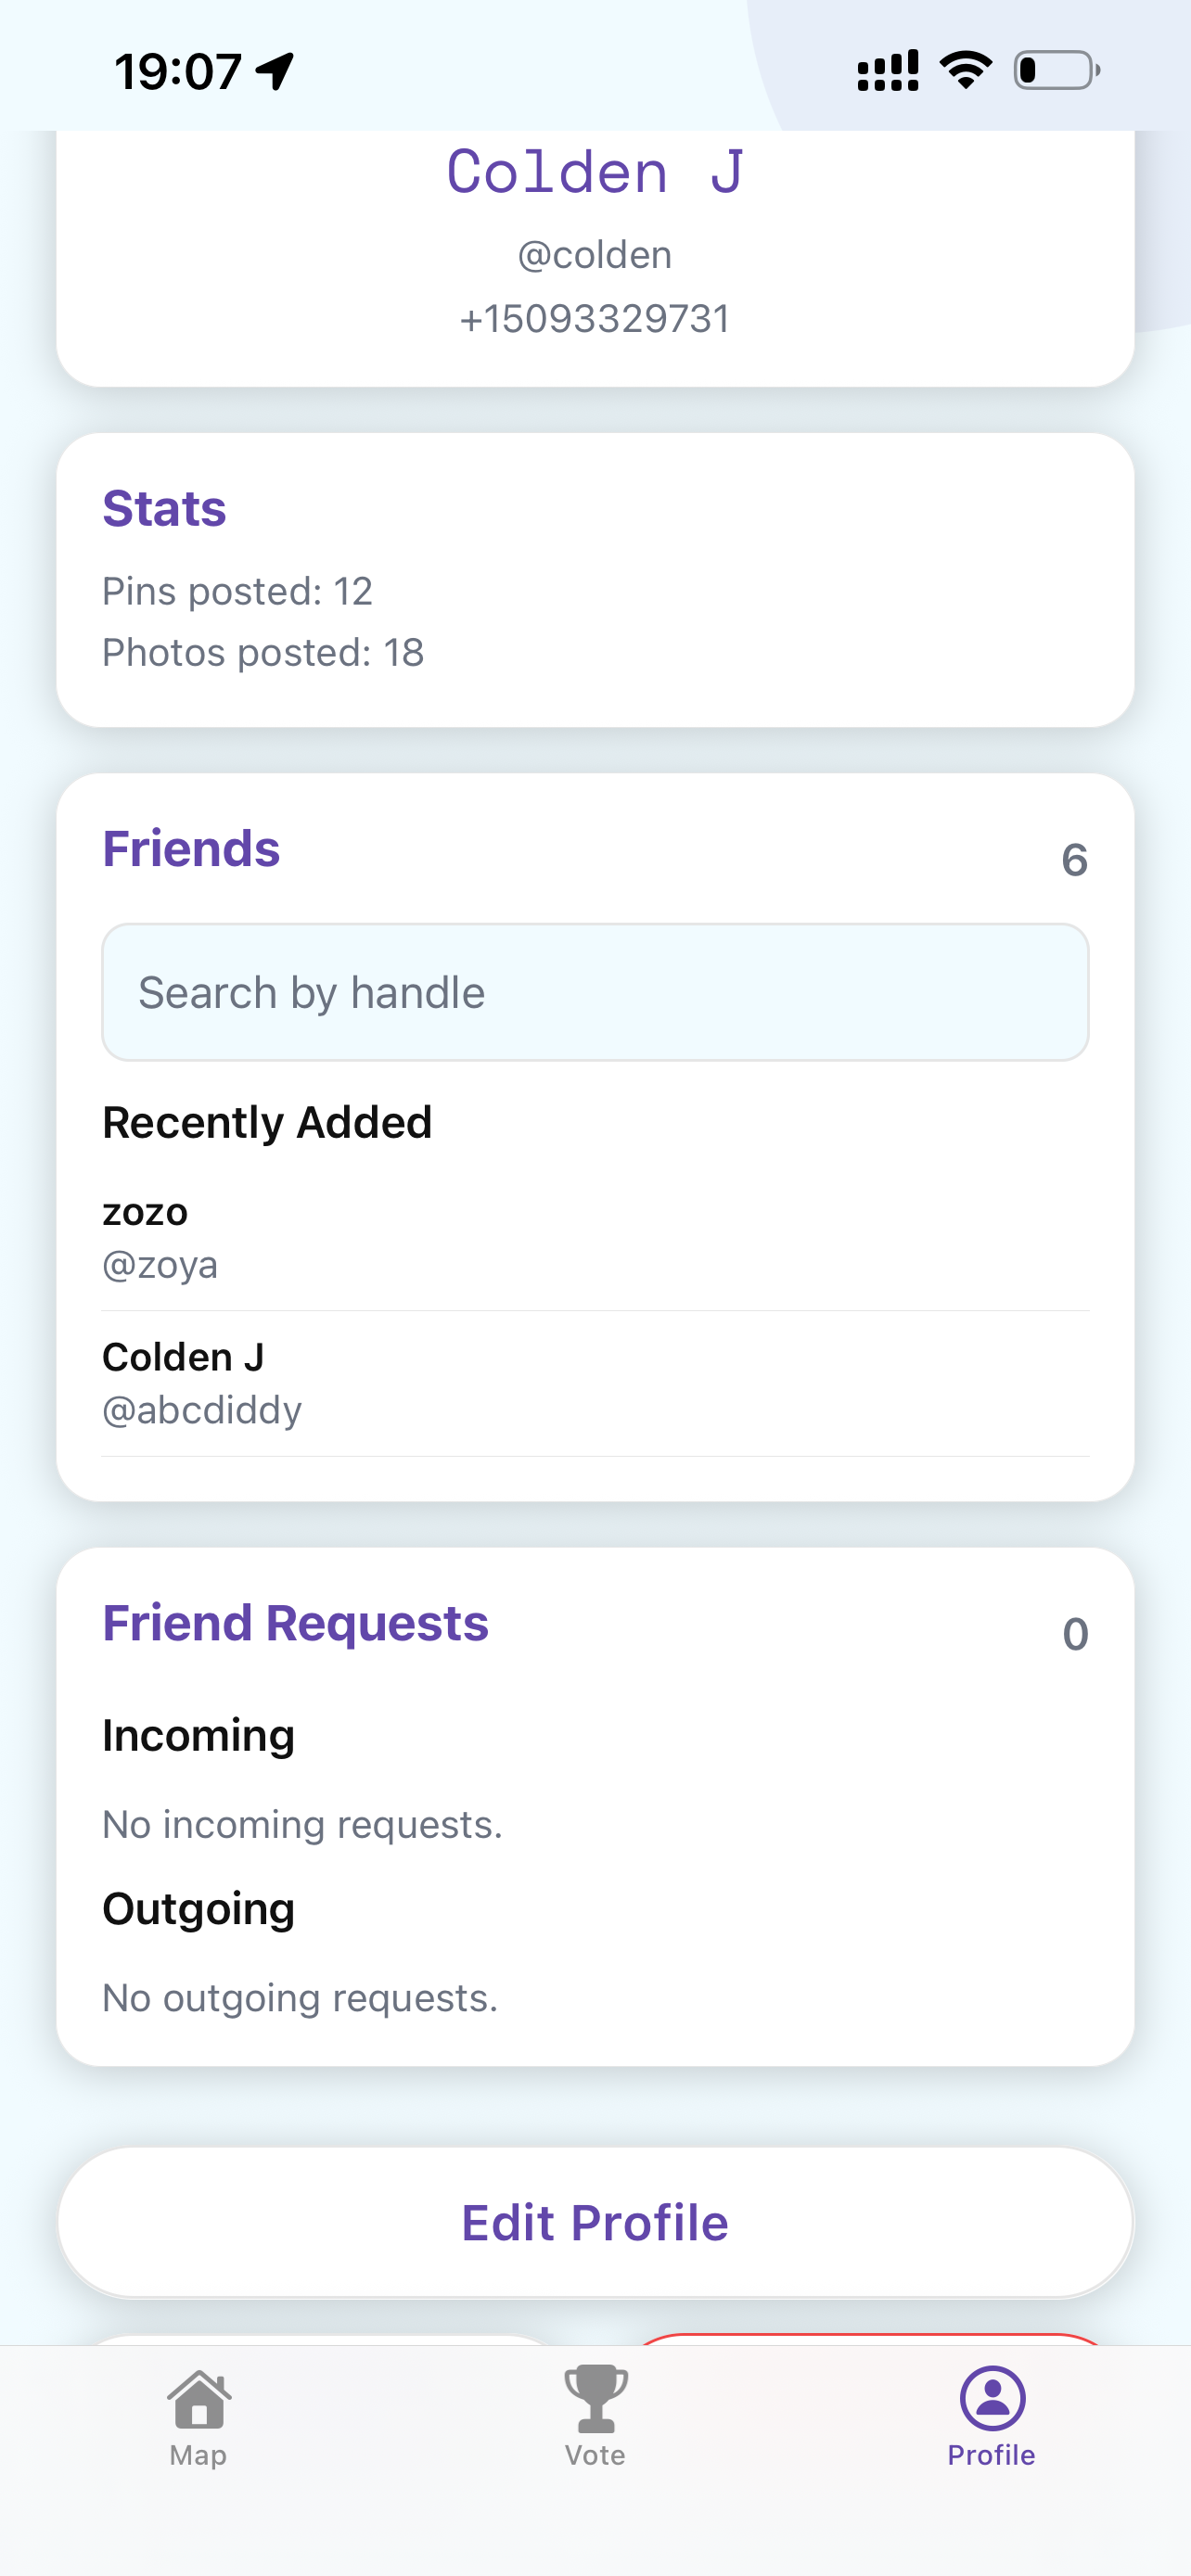
\includegraphics[width=\linewidth]{UserProfile.PNG}
    \caption{User profile with friends. \textit{(Current profile view, showing the friends system and user identity details.)}}
    \label{fig:user-profile}
  \end{minipage}
\end{figure}

\begin{figure}[!htbp]
  \centering
  \begin{minipage}[t]{0.48\linewidth}
    \centering
    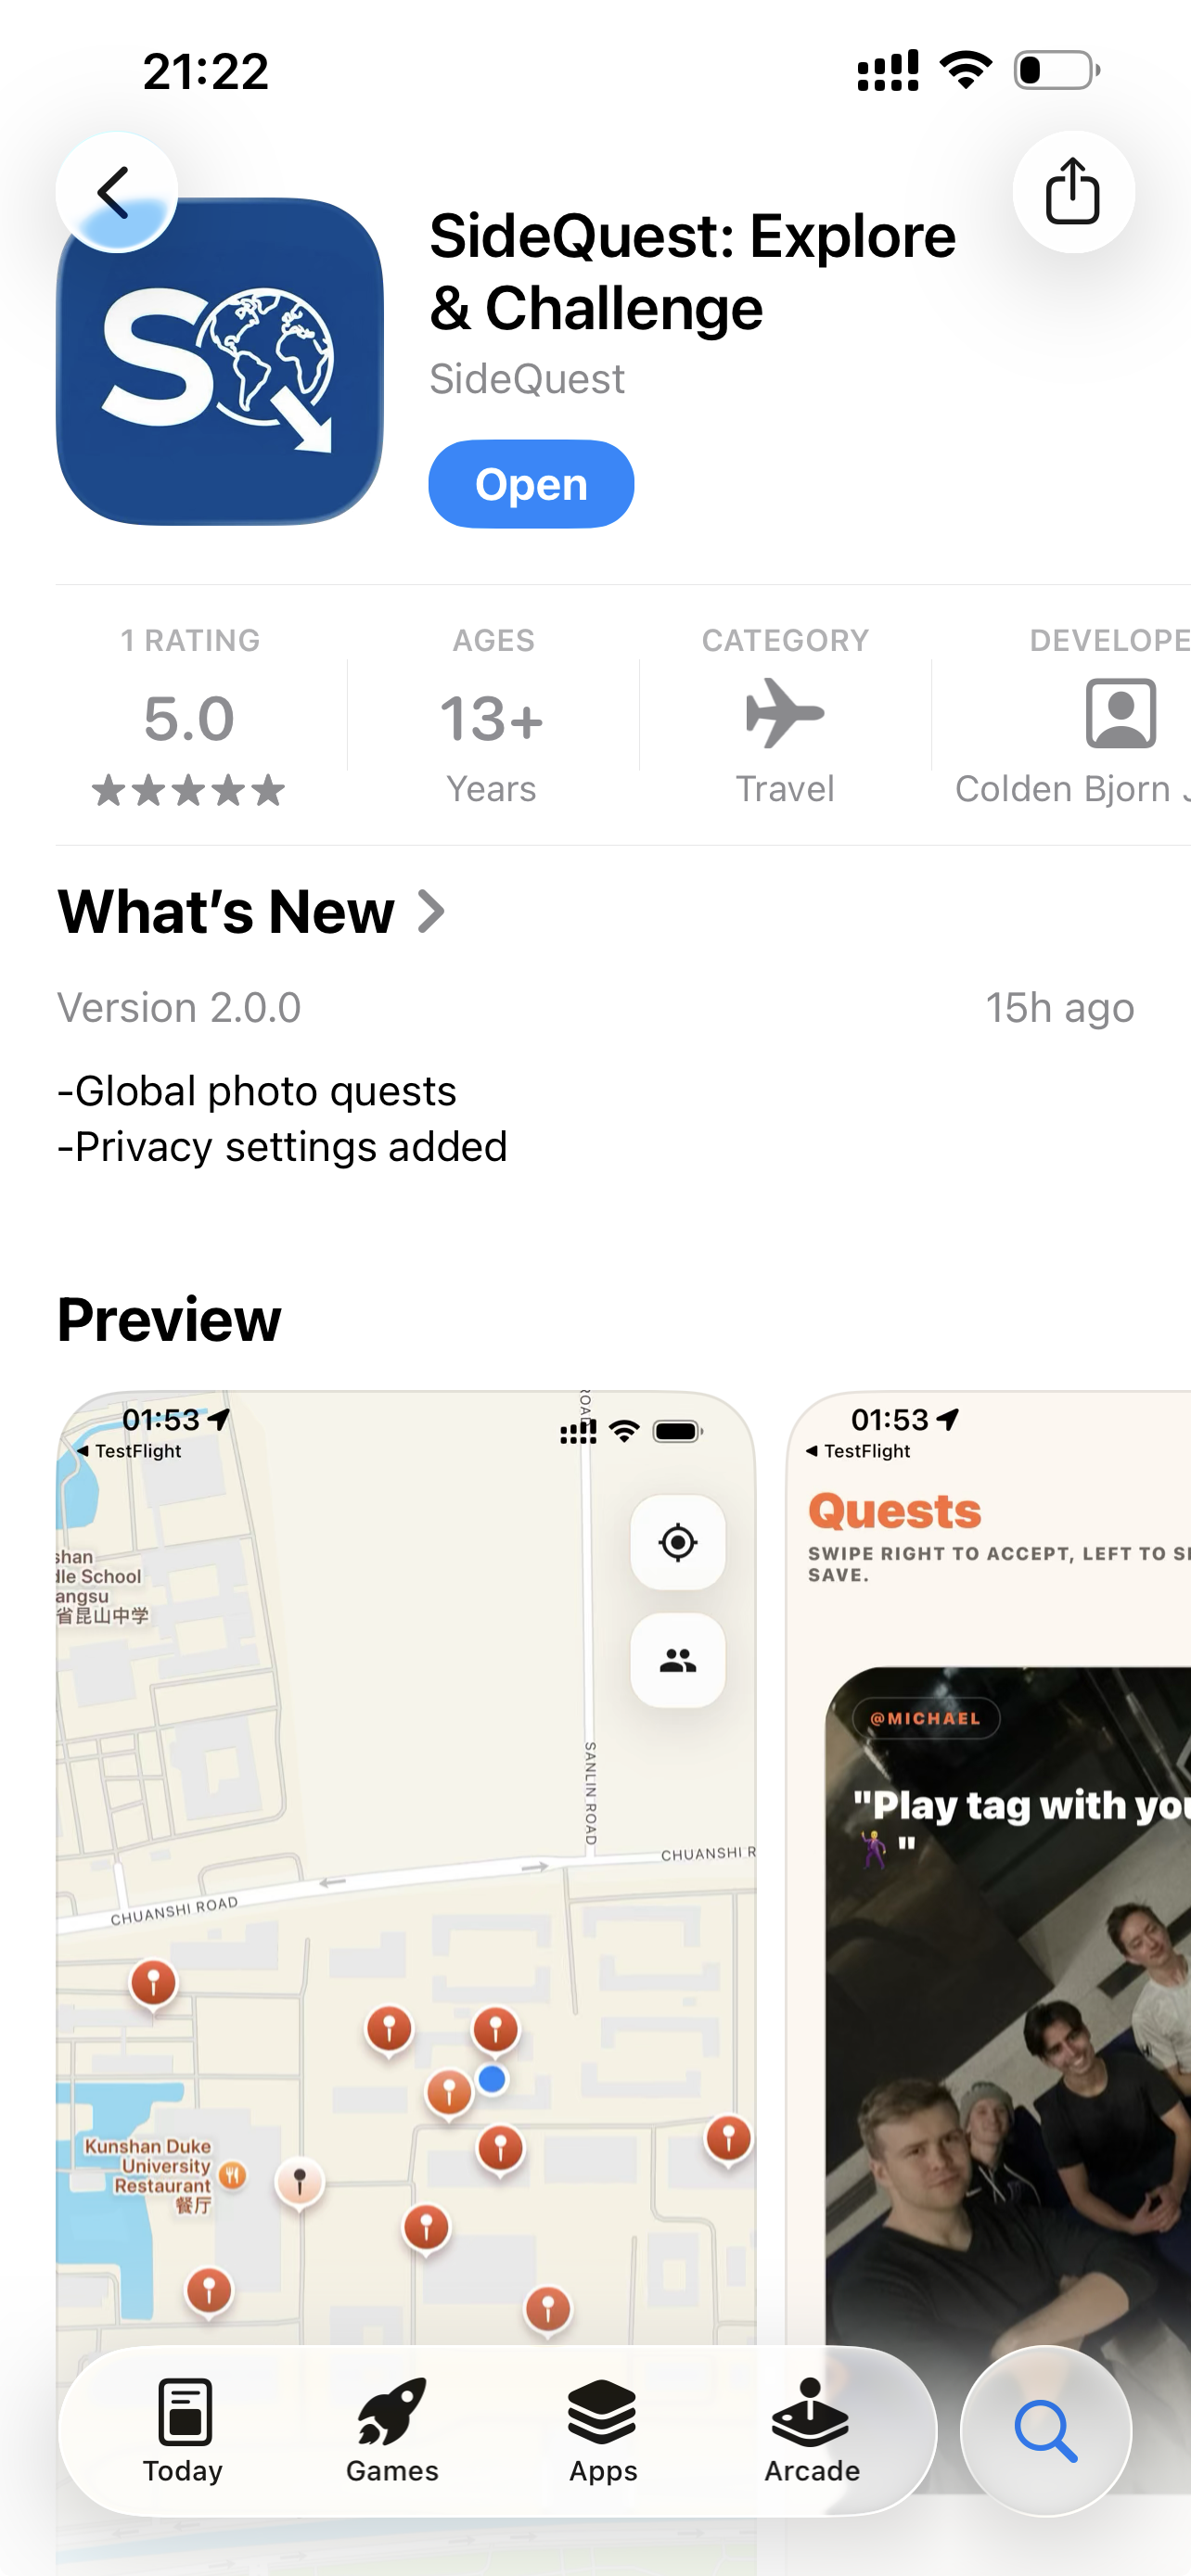
\includegraphics[width=\linewidth]{AppPhotos/sidequest_appstorepage.png}
    \caption{SideQuest App Store page. \textit{(Public listing for SideQuest: Explore \& Challenge.)}}
    \label{fig:appphotos-appstore-page}
  \end{minipage}\hfill
  \begin{minipage}[t]{0.48\linewidth}
    \centering
    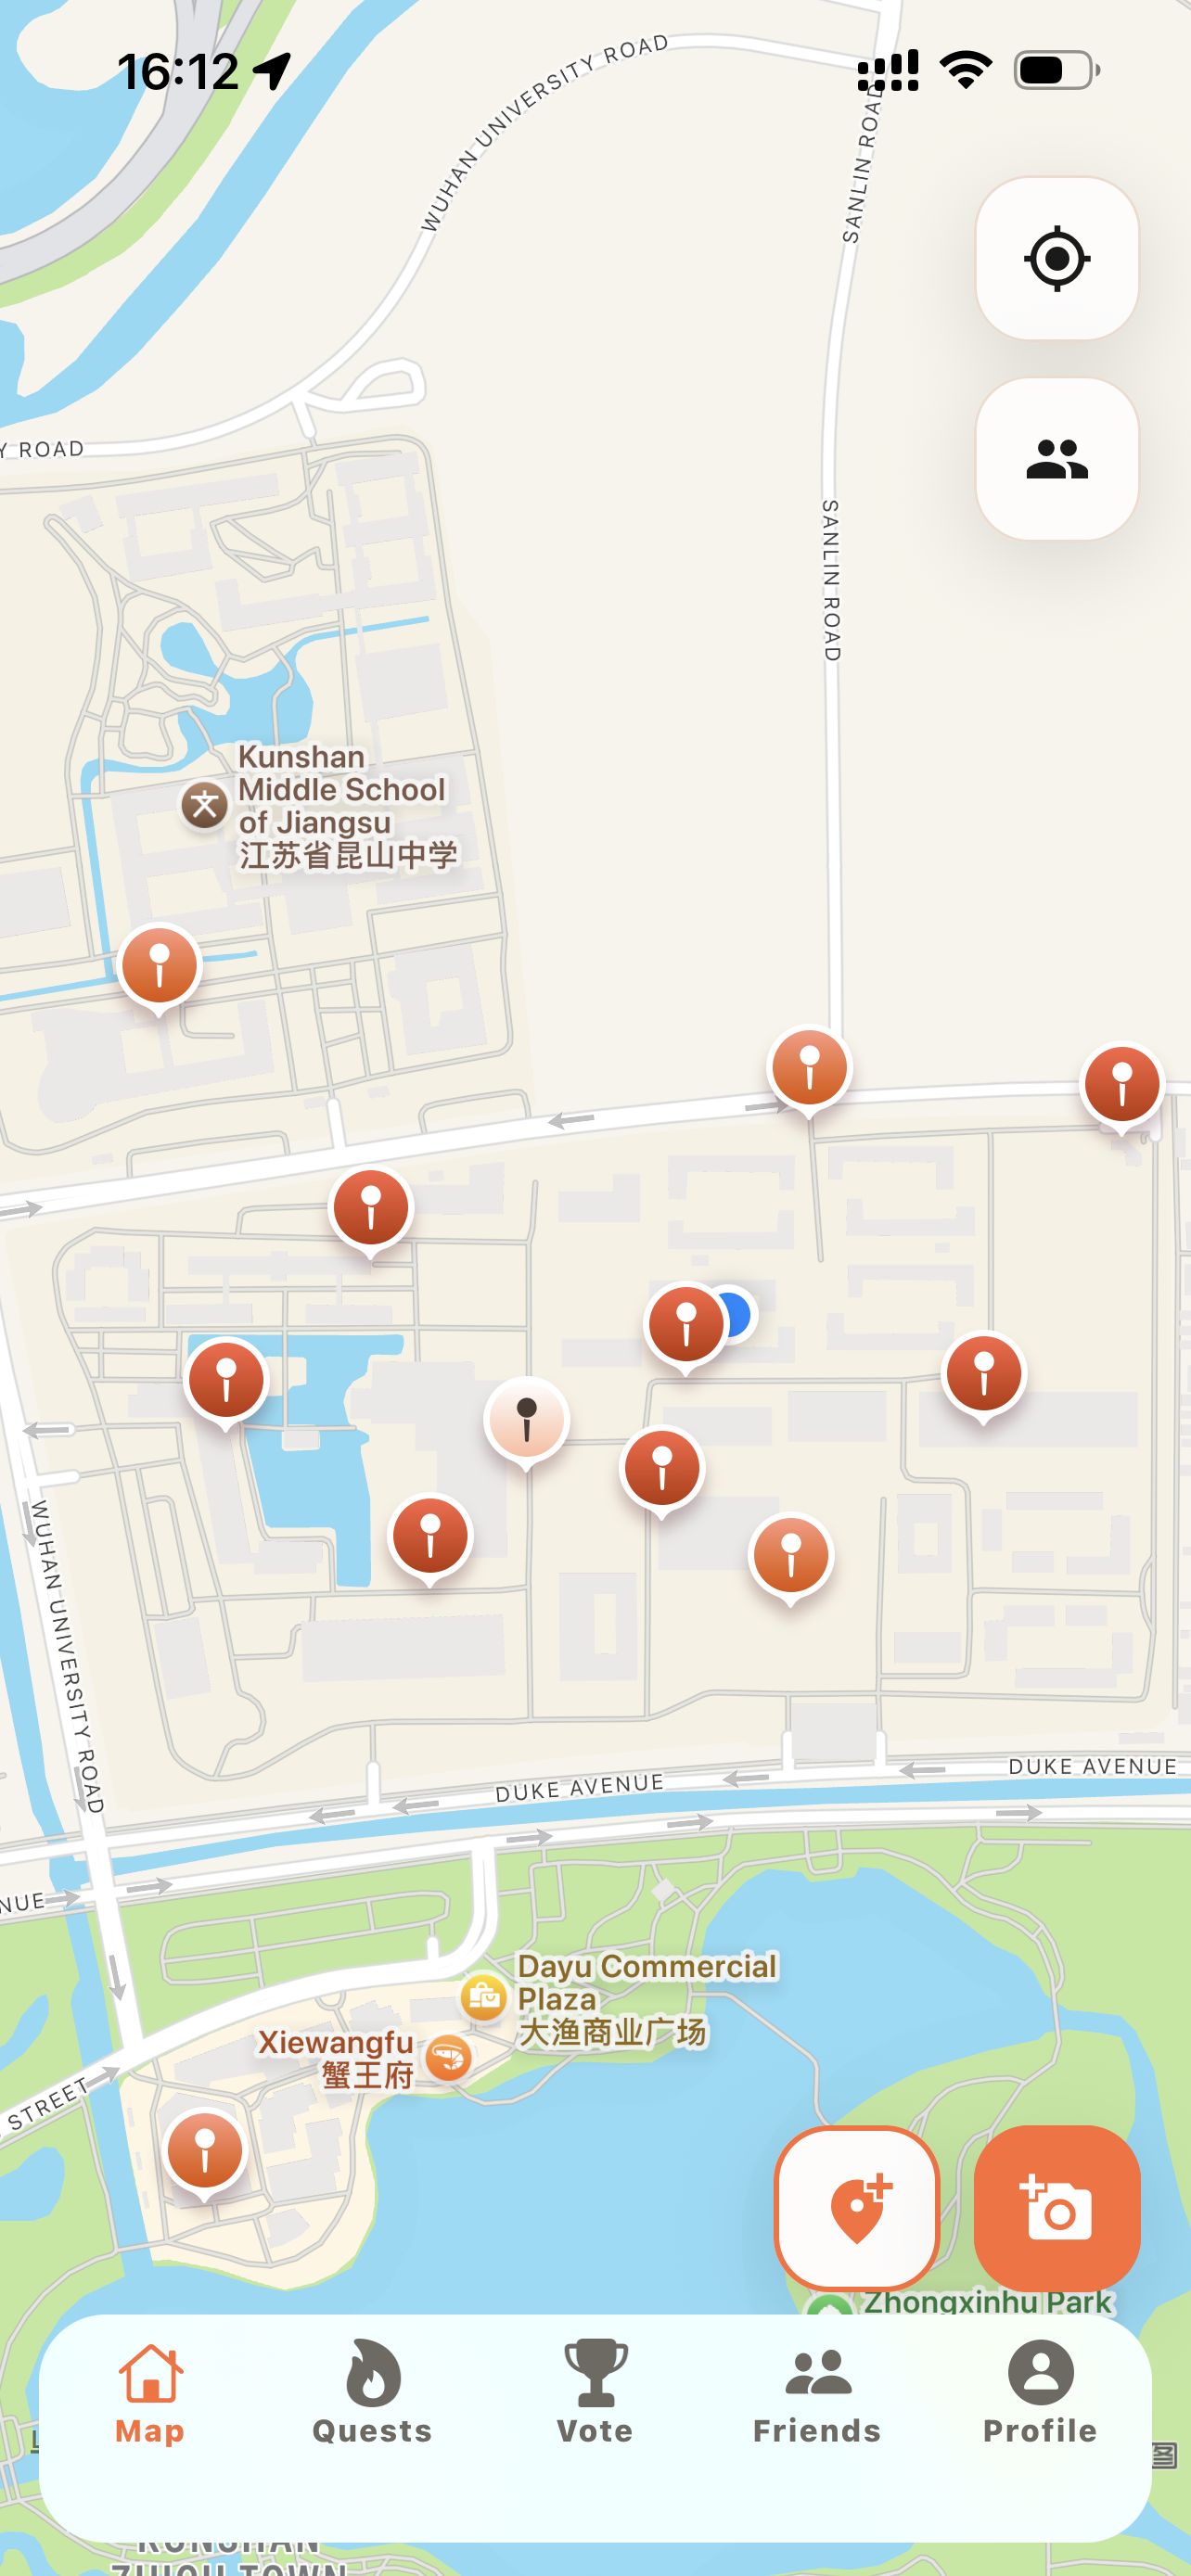
\includegraphics[width=\linewidth]{AppPhotos/Sidequest_Map.PNG}
    \caption{In-app map view. \textit{(Primary live map screen used to discover nearby Quests.)}}
    \label{fig:appphotos-map}
  \end{minipage}
\end{figure}

\begin{figure}[!htbp]
  \centering
  \begin{minipage}[t]{0.48\linewidth}
    \centering
    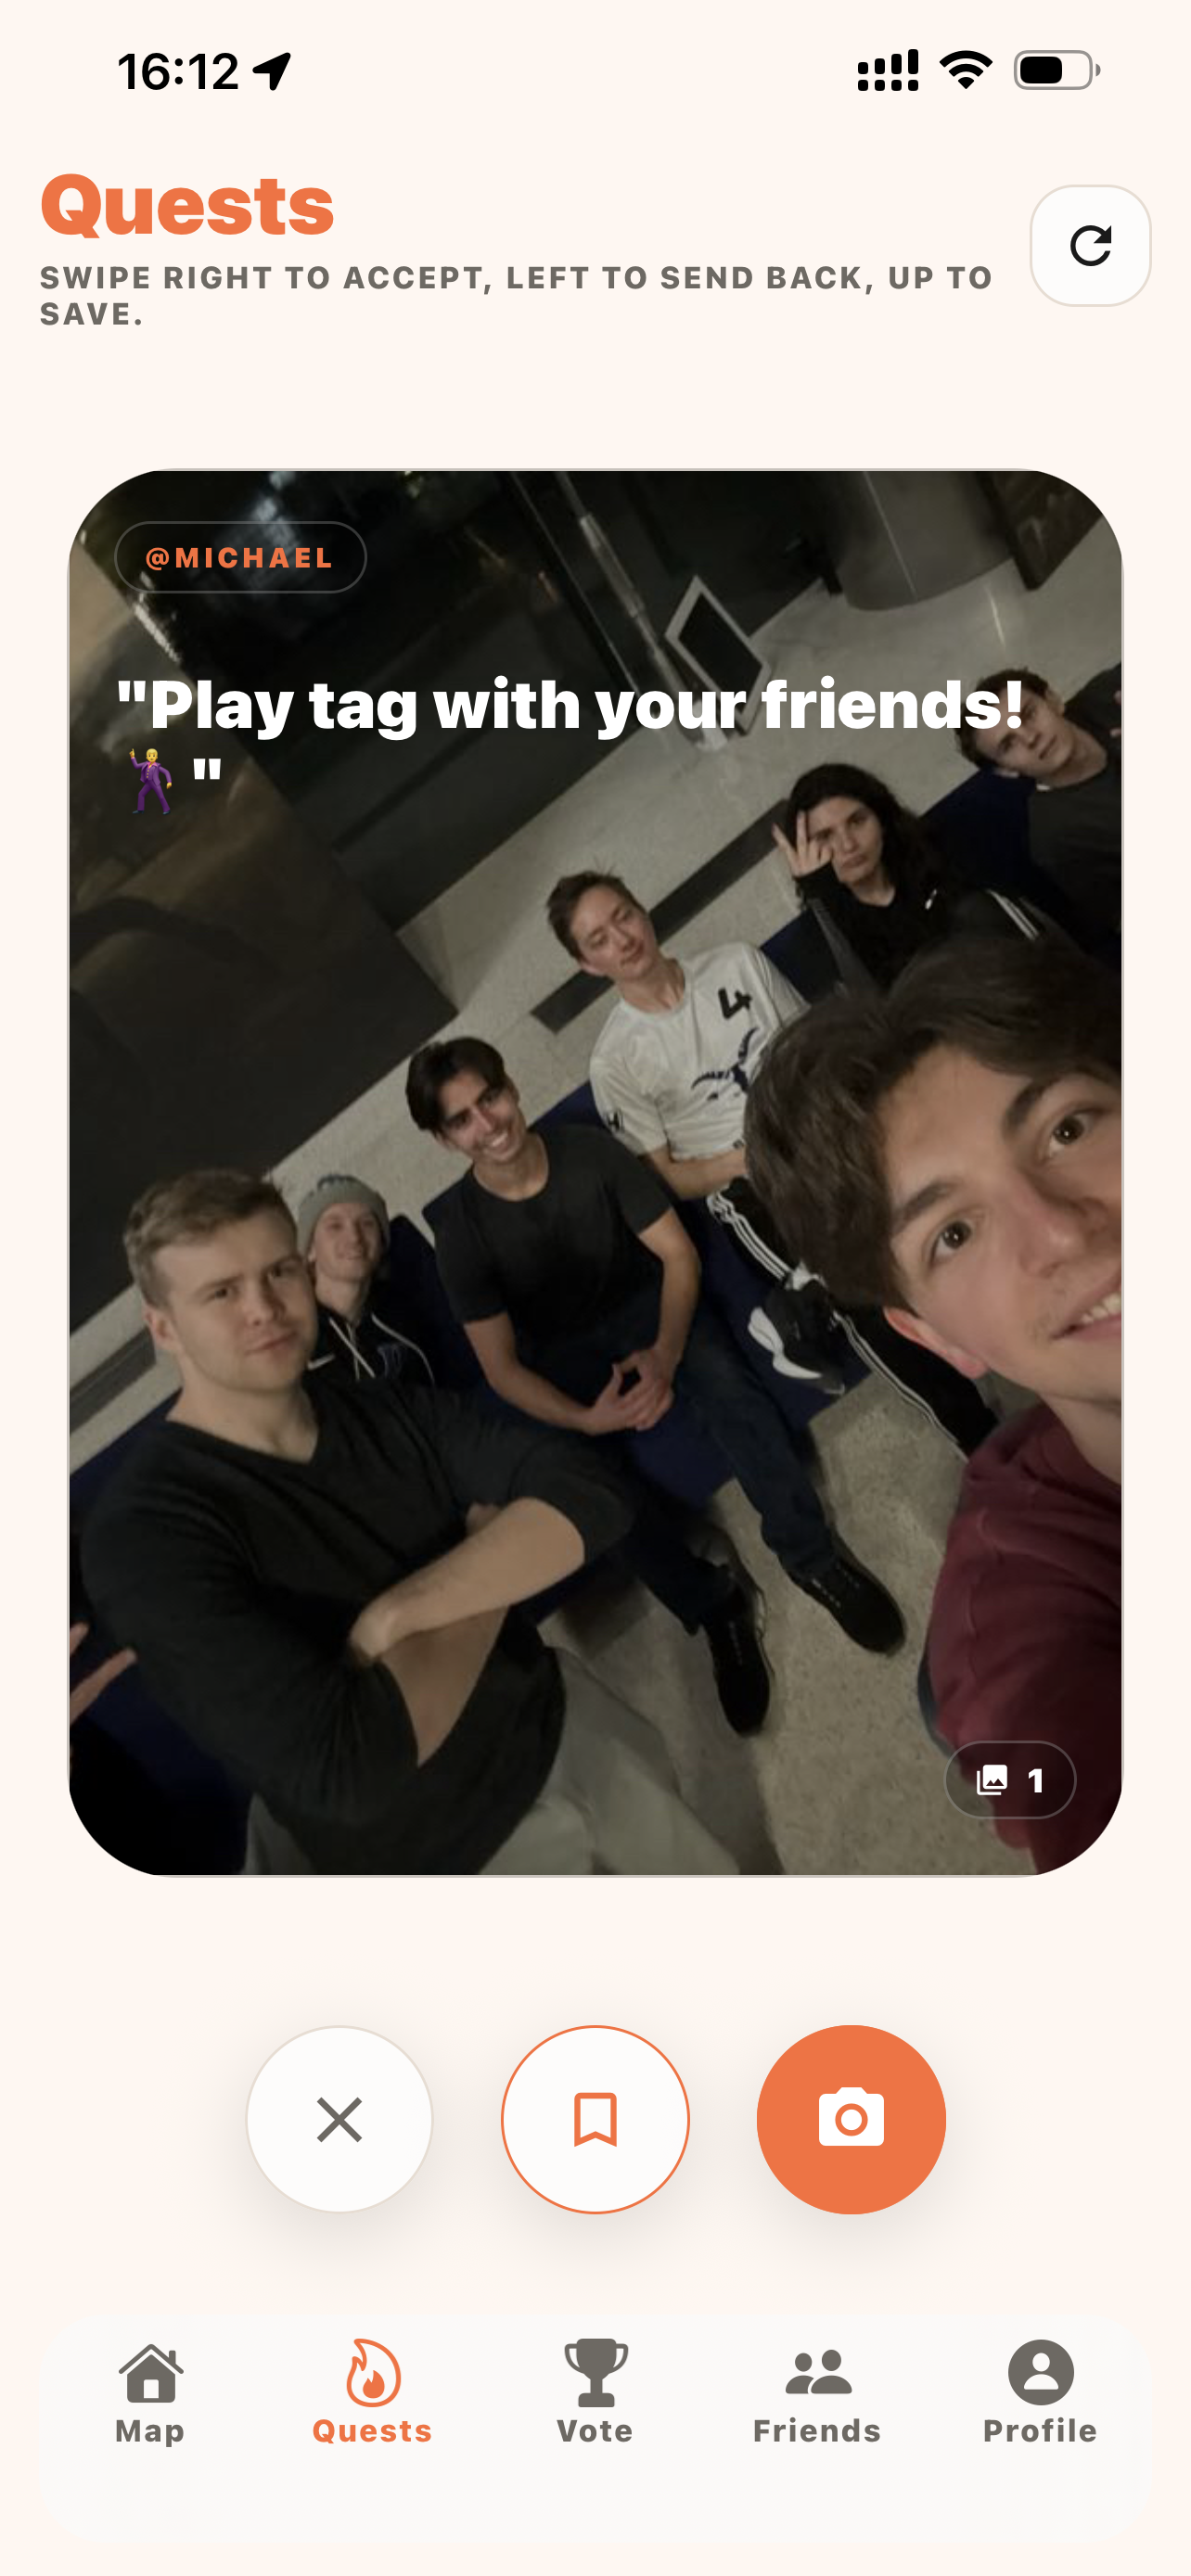
\includegraphics[width=\linewidth]{AppPhotos/Sidequest_Quests.PNG}
    \caption{Quests feed view. \textit{(Quest browsing interface for challenge discovery and participation.)}}
    \label{fig:appphotos-quests}
  \end{minipage}\hfill
  \begin{minipage}[t]{0.48\linewidth}
    \centering
    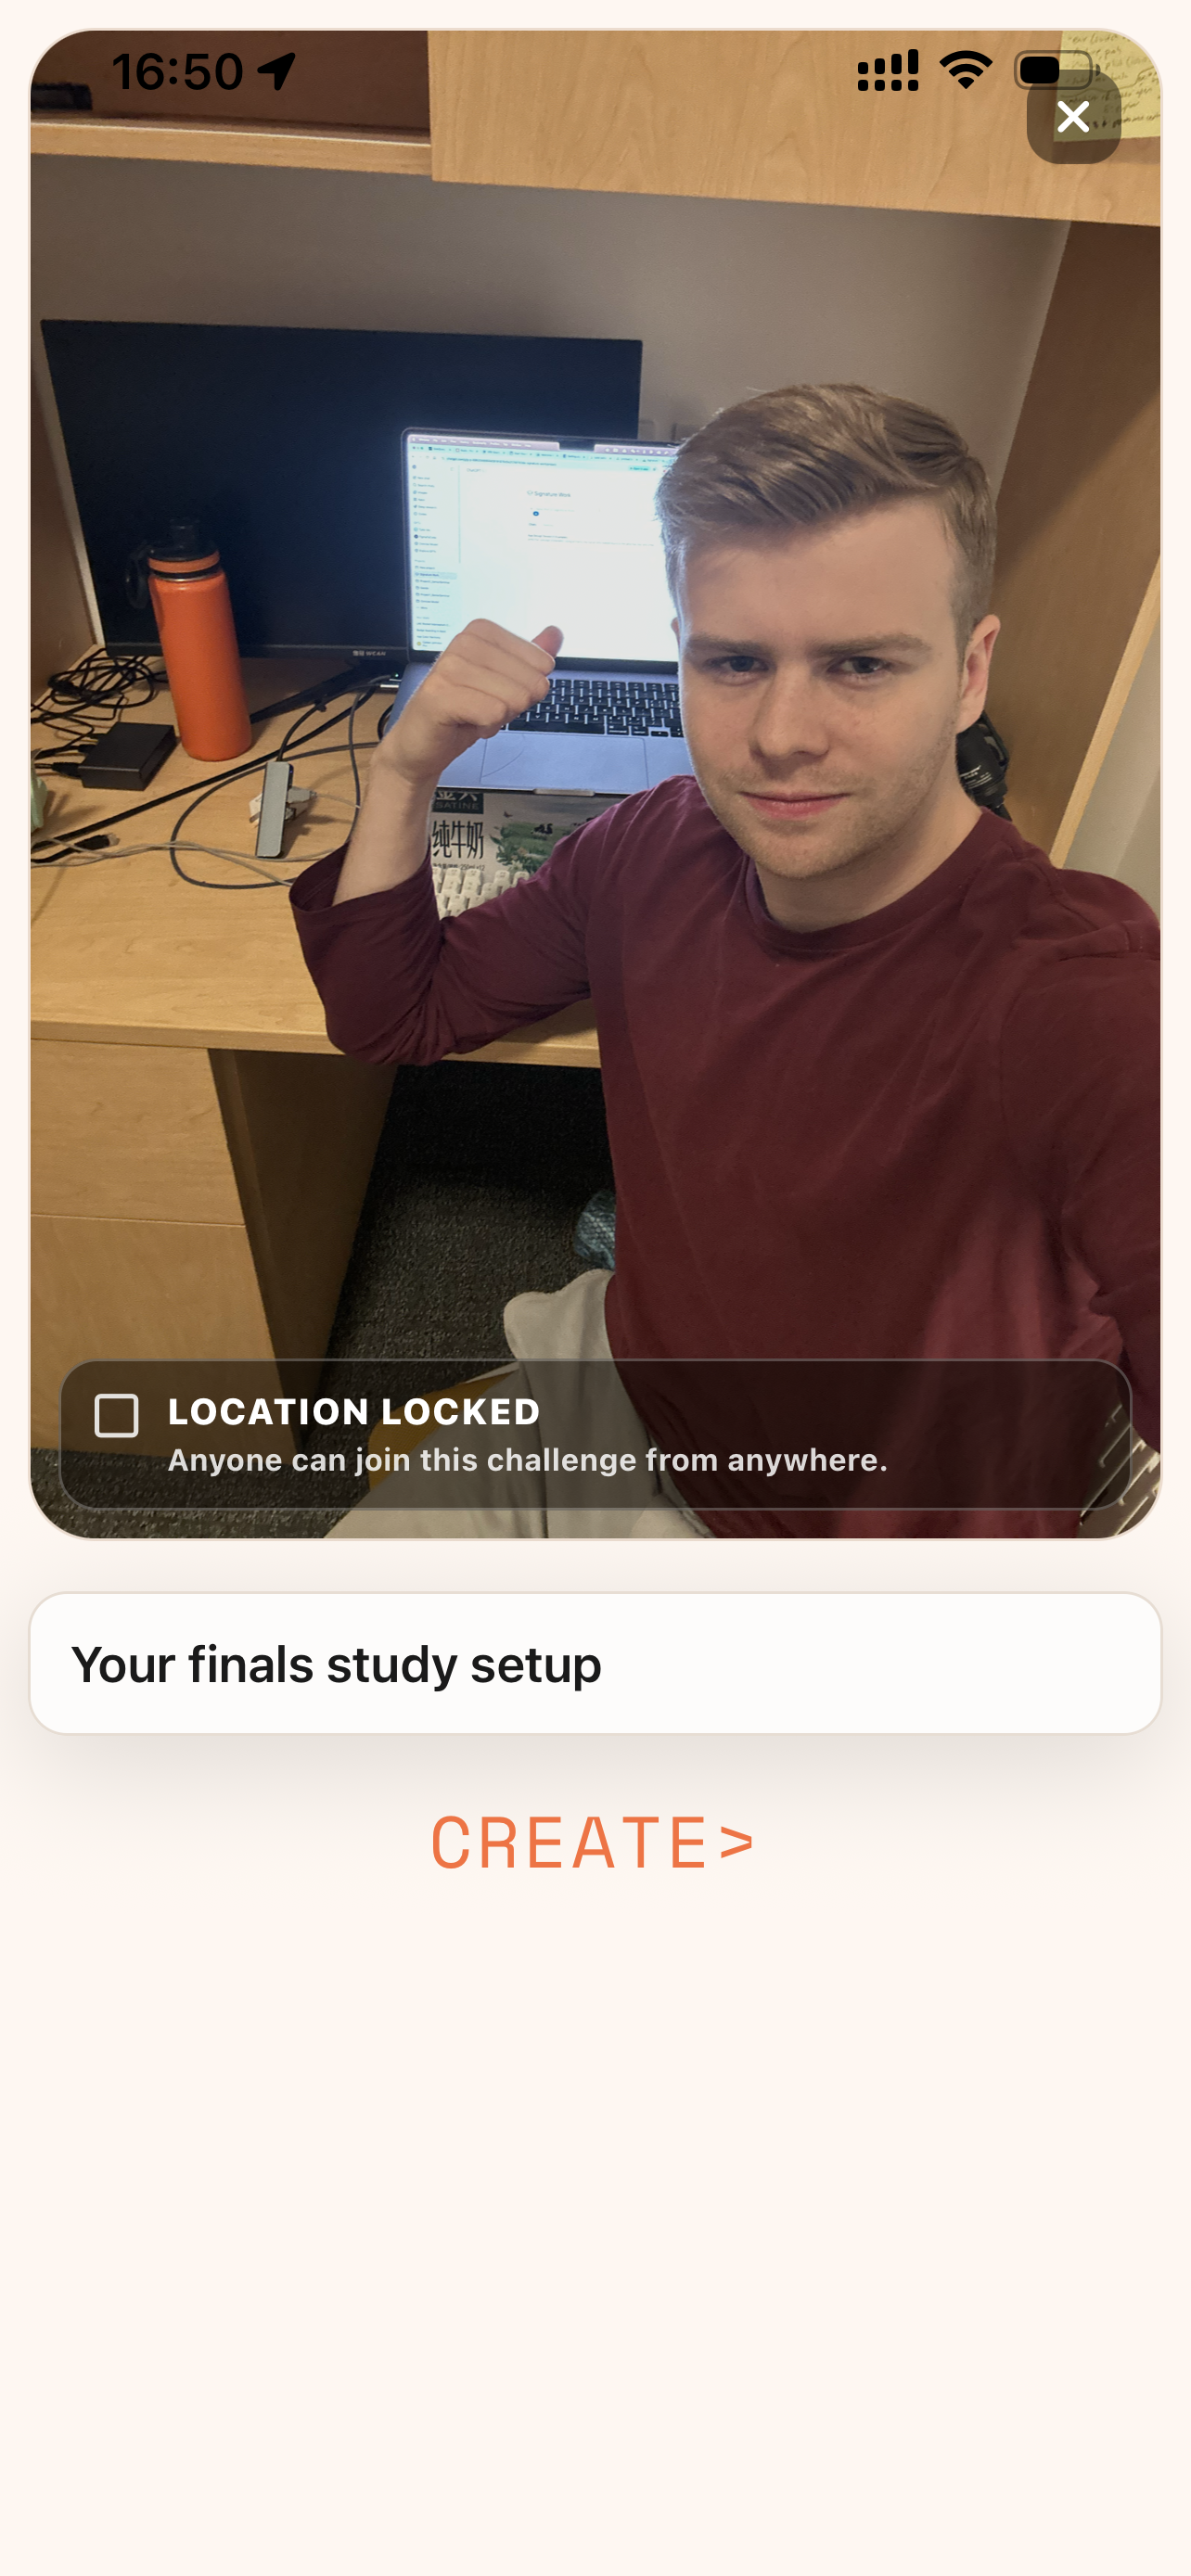
\includegraphics[width=\linewidth]{AppPhotos/Sidequest_ChallengeCreation.PNG}
    \caption{Challenge creation flow. \textit{(UI for creating a new Quest with image and prompt.)}}
    \label{fig:appphotos-challenge-creation}
  \end{minipage}
\end{figure}

\begin{figure}[!htbp]
  \centering
  \begin{minipage}[t]{0.48\linewidth}
    \centering
    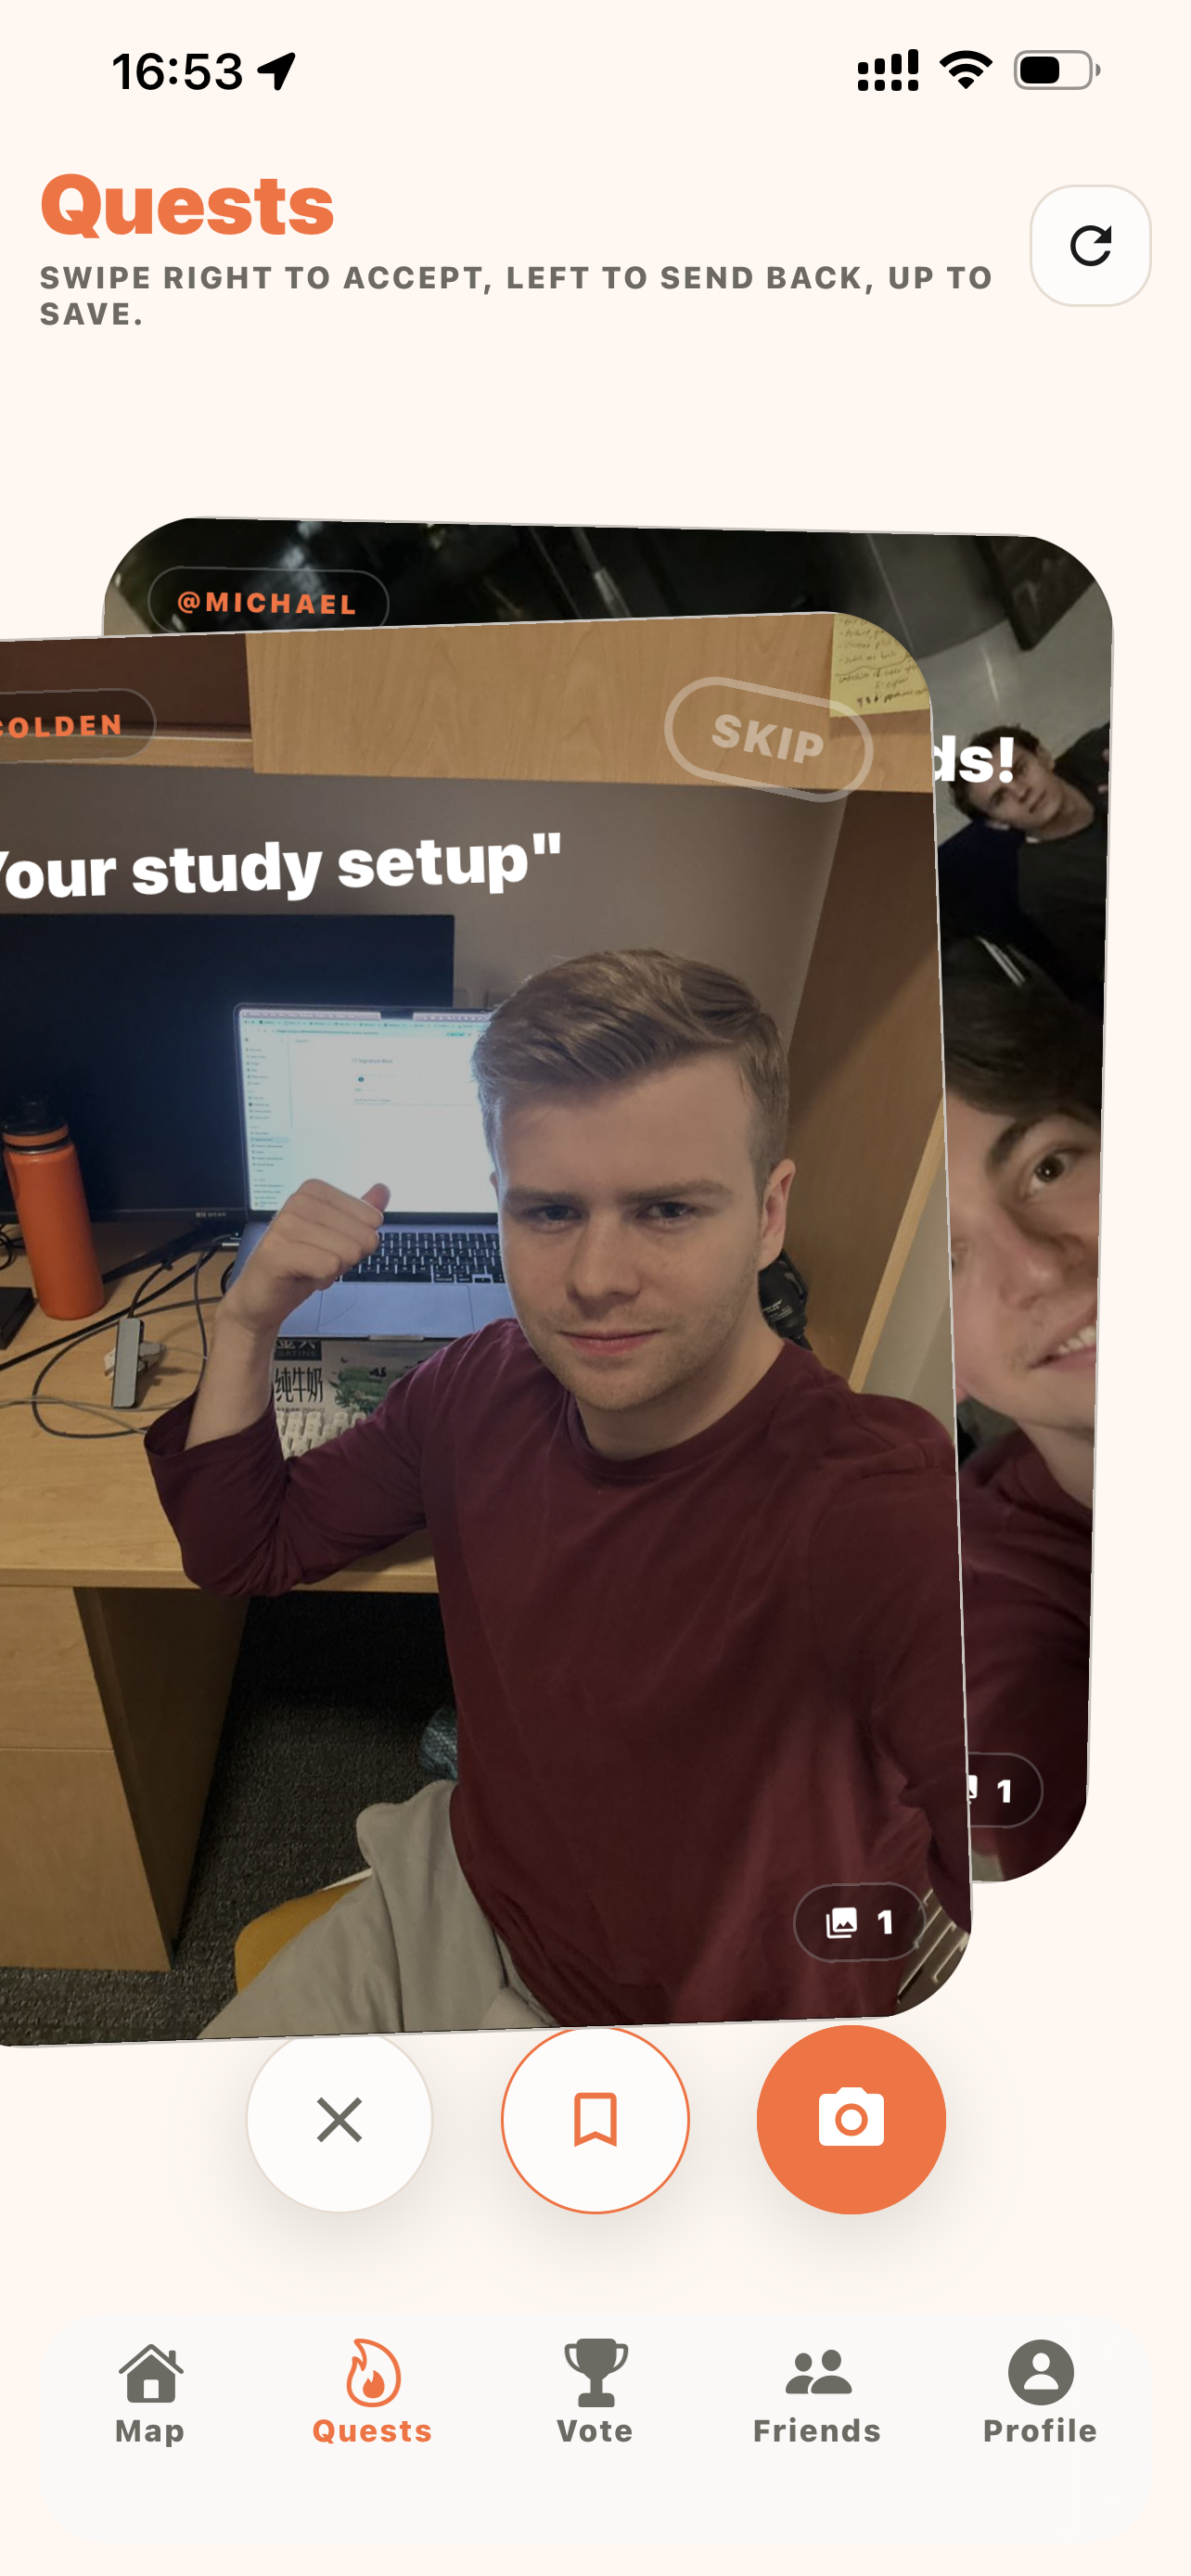
\includegraphics[width=\linewidth]{AppPhotos/SideQuest_ChallengeAppearsinQuests.PNG}
    \caption{Challenge appears in Quest list. \textit{(Newly created challenge surfaced to other users in the feed.)}}
    \label{fig:appphotos-challenge-appears}
  \end{minipage}\hfill
  \begin{minipage}[t]{0.48\linewidth}
    \centering
    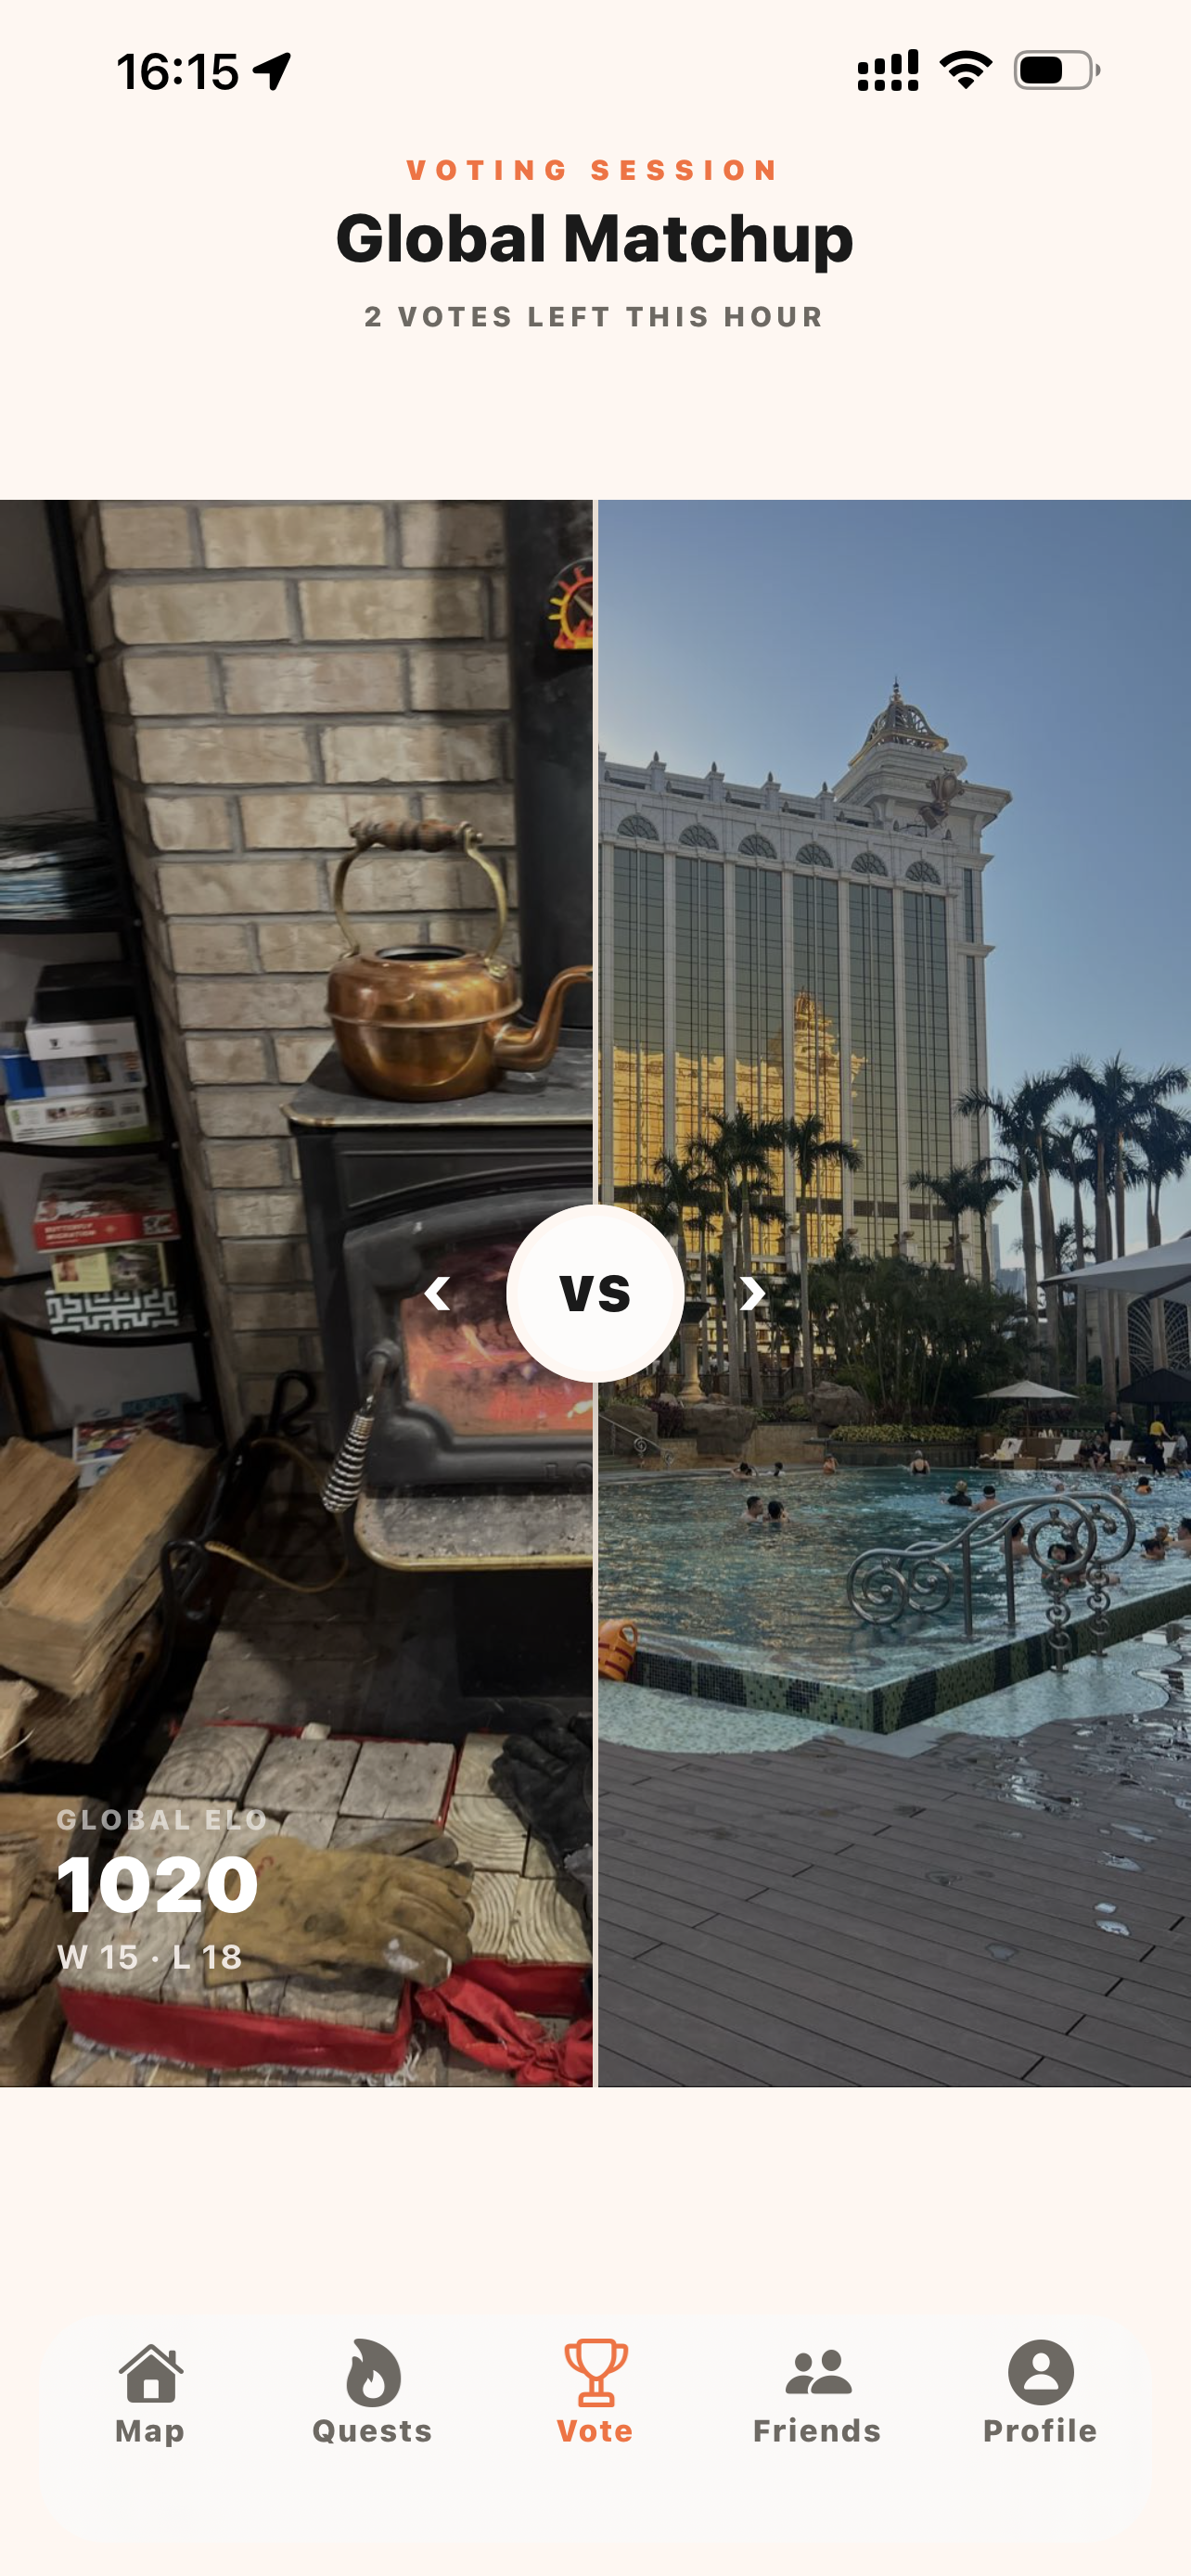
\includegraphics[width=\linewidth]{AppPhotos/Sidequest_voting.PNG}
    \caption{Voting and duel screen. \textit{(Head-to-head voting interface for community ranking.)}}
    \label{fig:appphotos-voting}
  \end{minipage}
\end{figure}

\begin{figure}[!htbp]
  \centering
  \begin{minipage}[t]{0.48\linewidth}
    \centering
    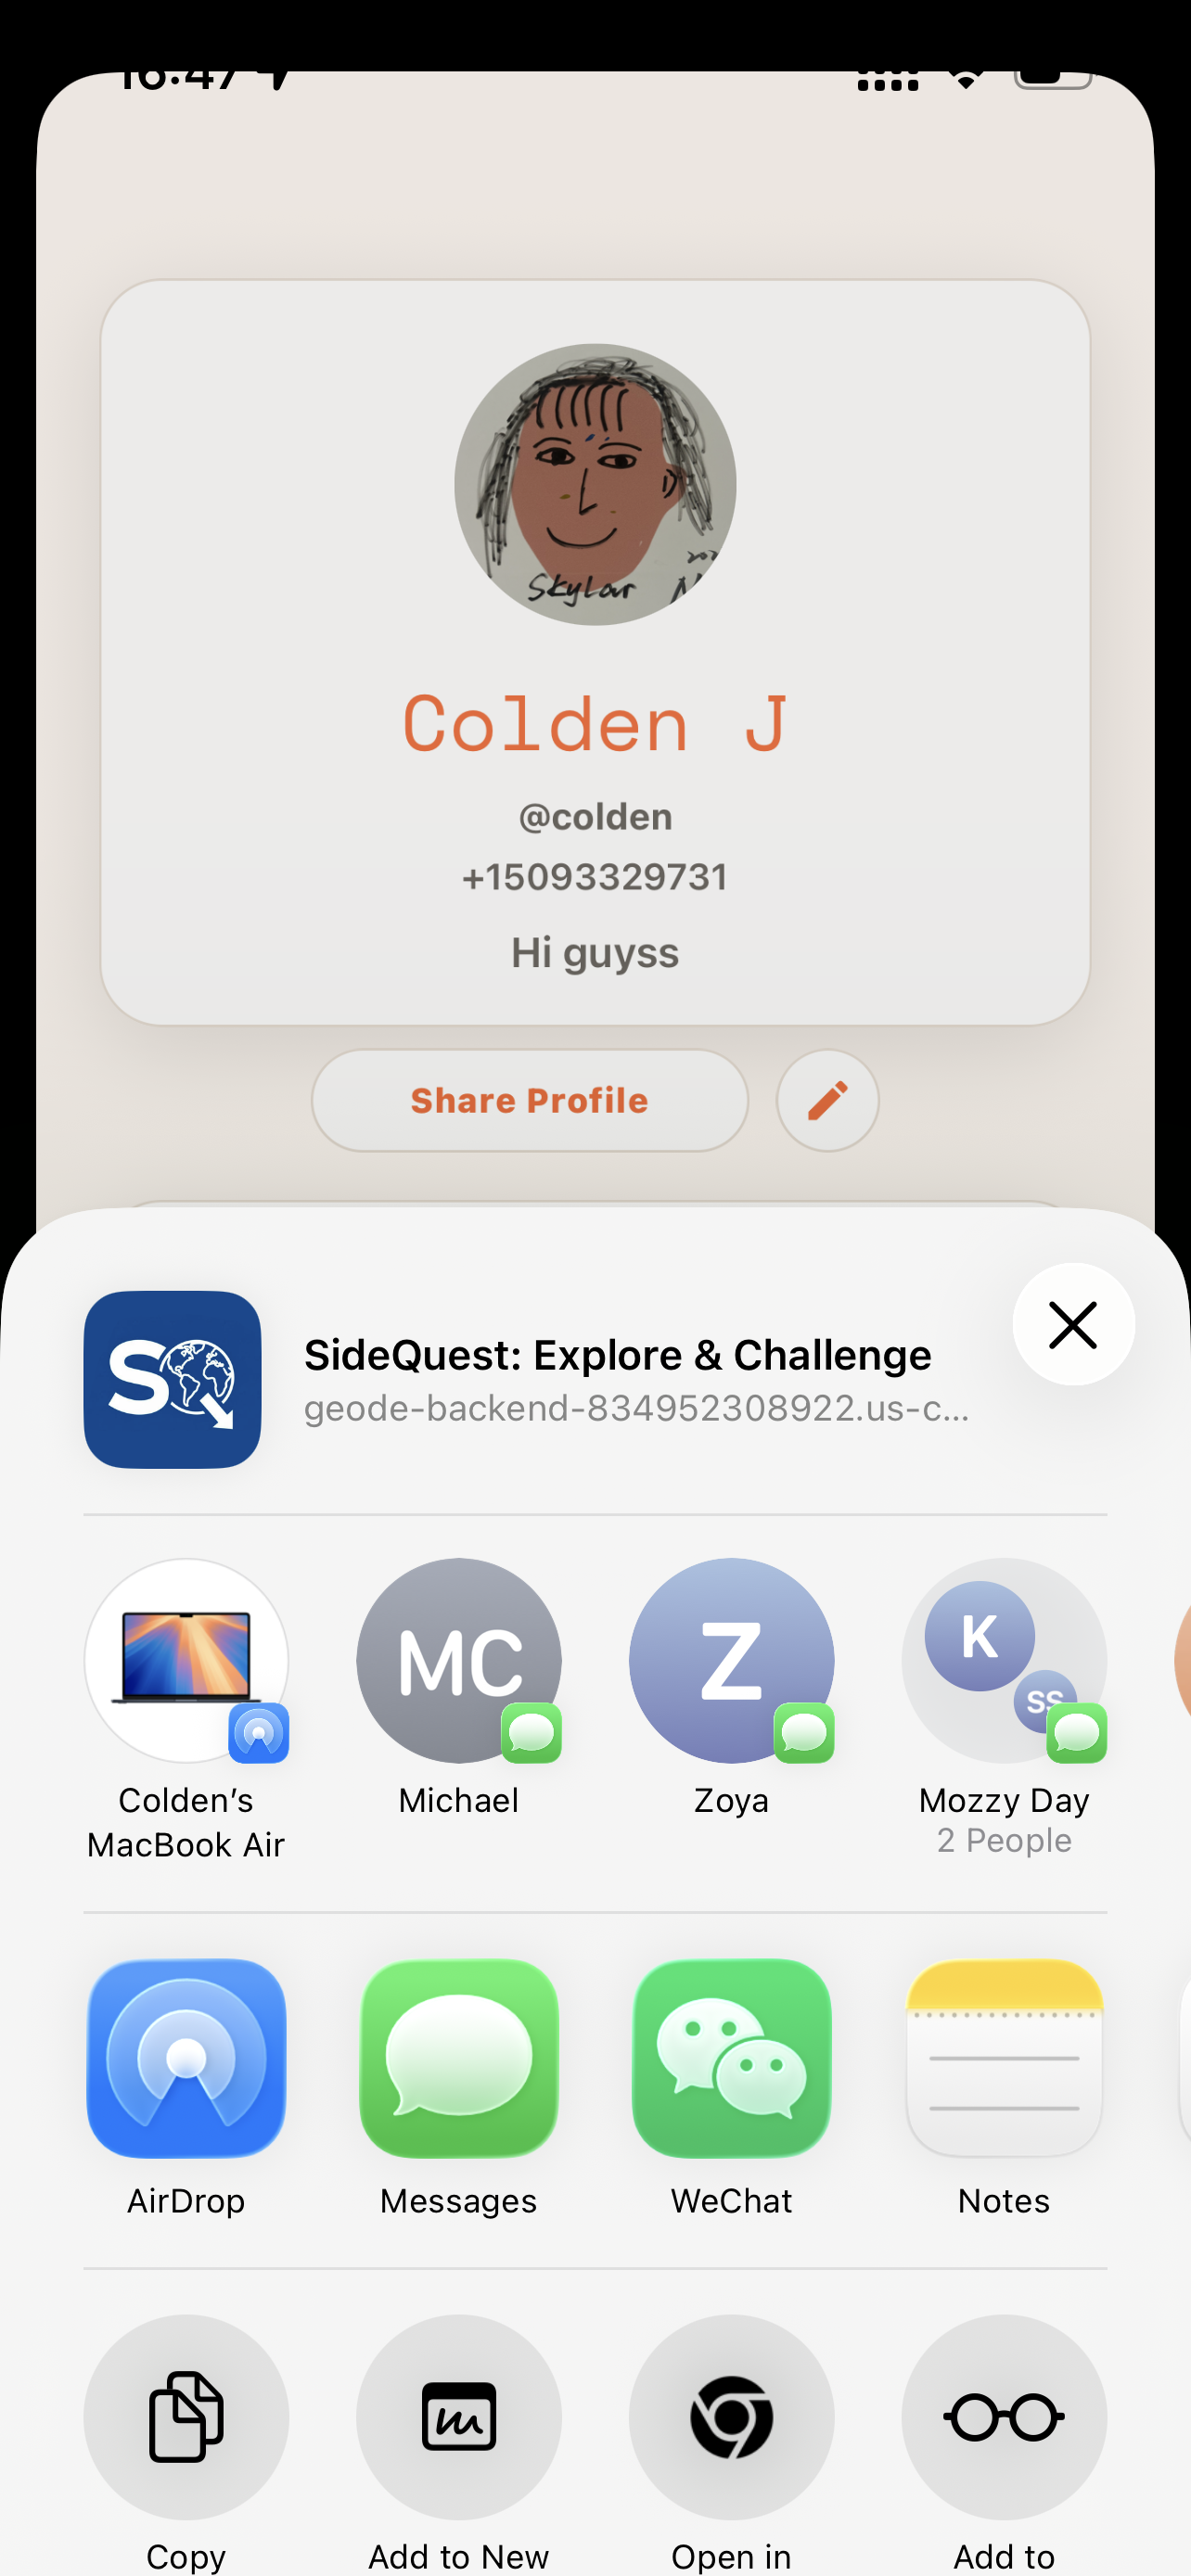
\includegraphics[width=\linewidth]{AppPhotos/Sidequest_Share.PNG}
    \caption{Quest sharing view. \textit{(Sharing interface to distribute challenges with friends.)}}
    \label{fig:appphotos-share}
  \end{minipage}\hfill
  \begin{minipage}[t]{0.48\linewidth}
    \centering
    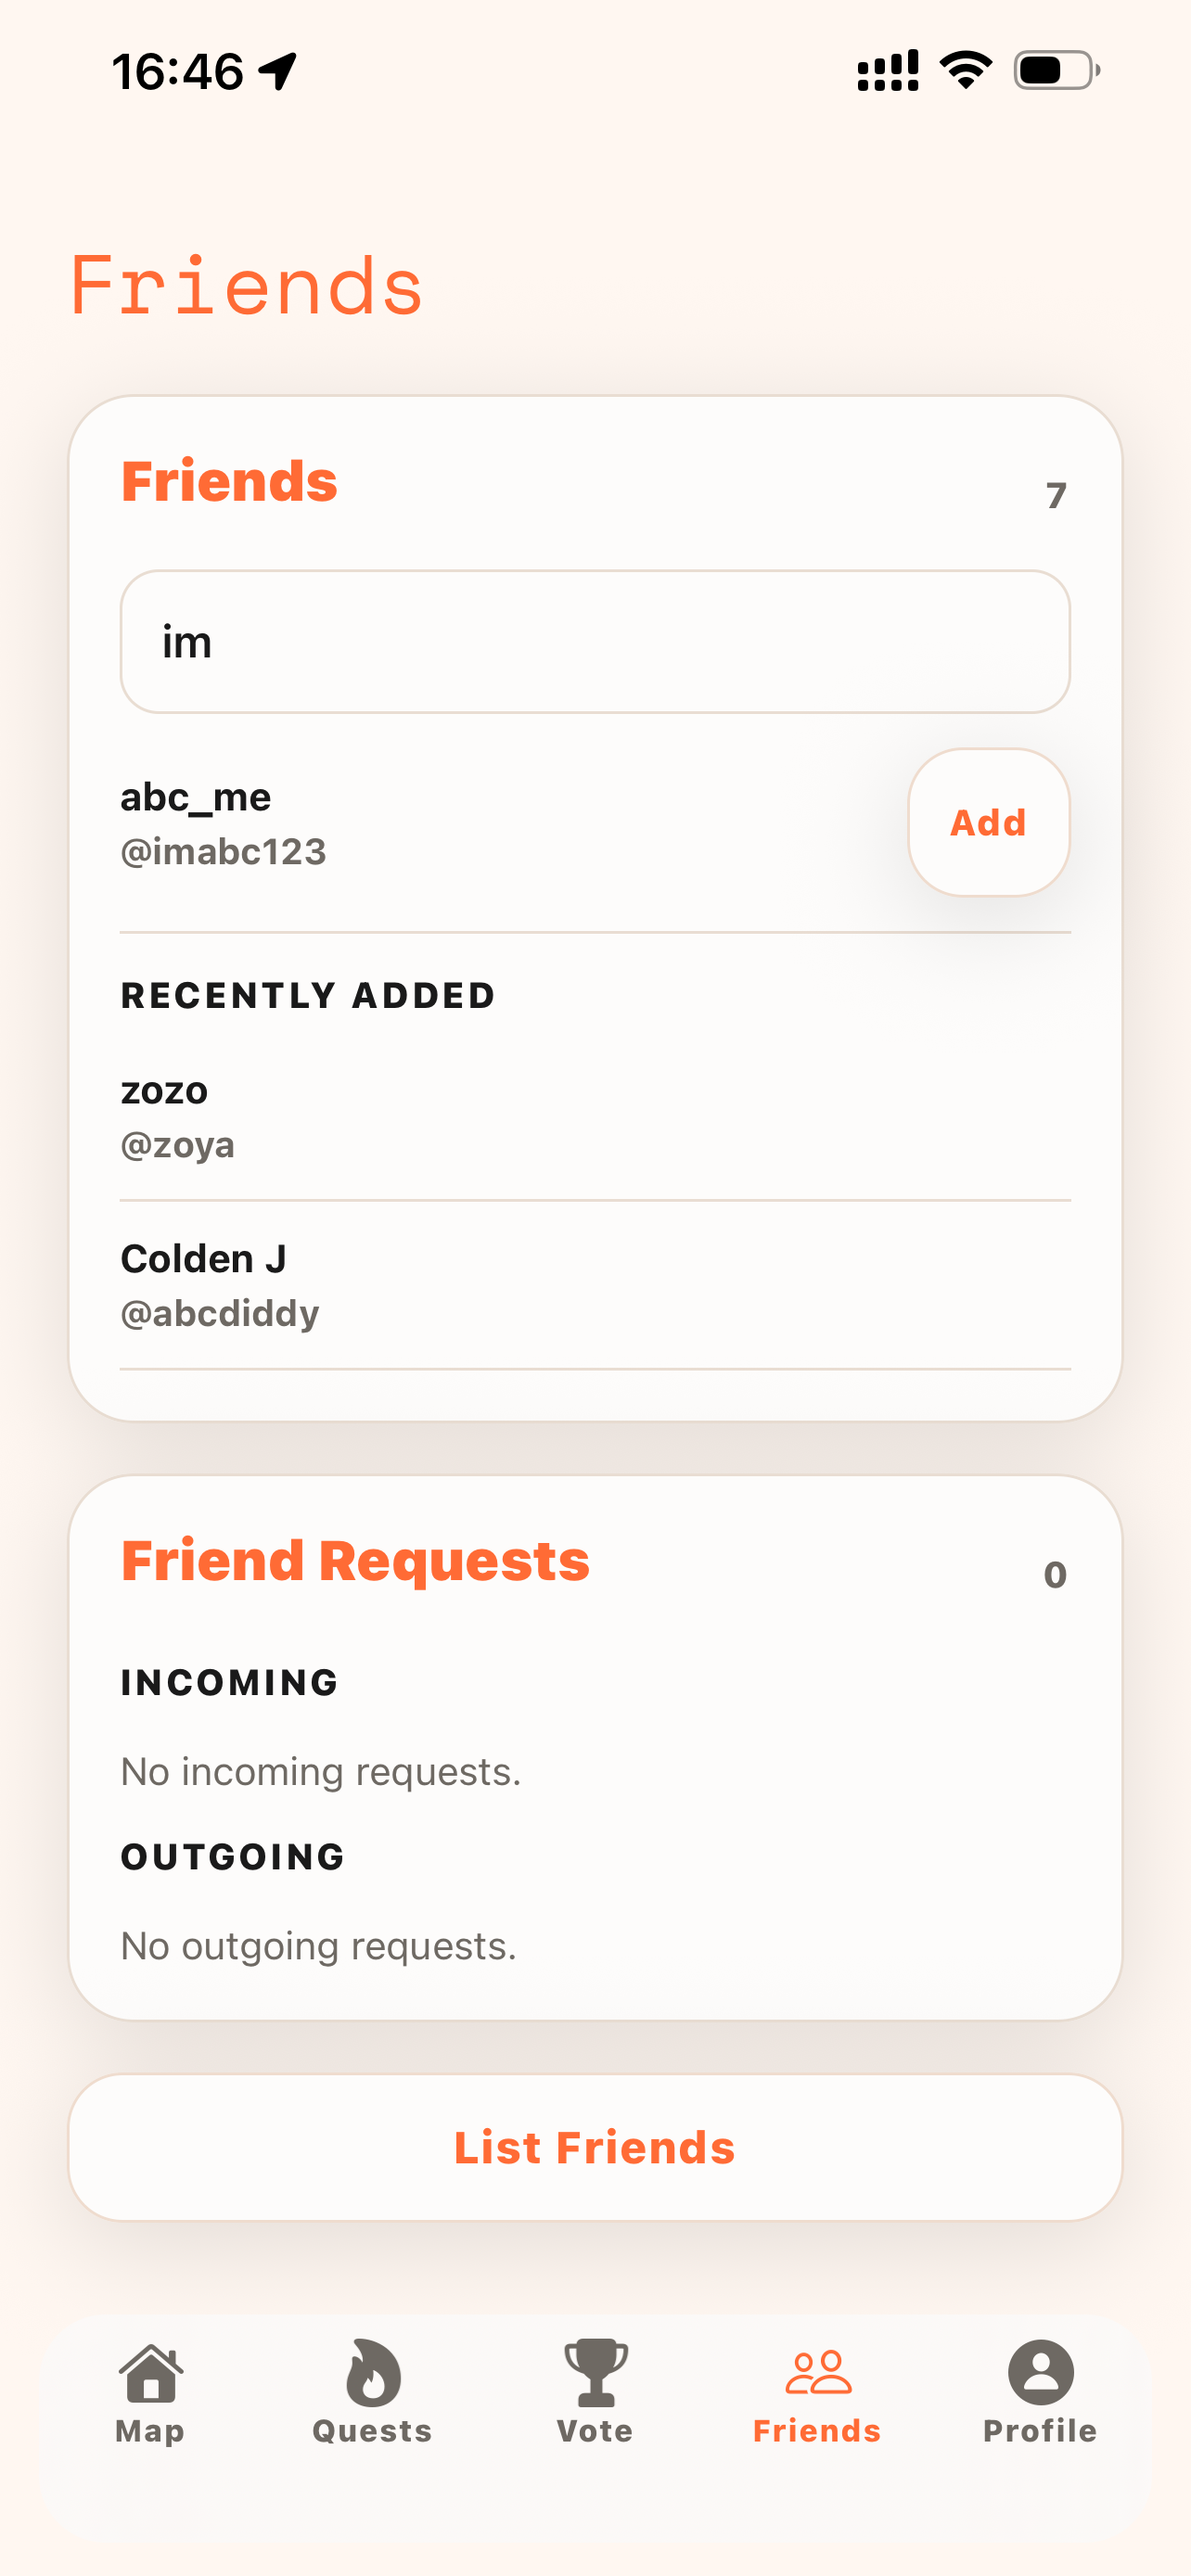
\includegraphics[width=\linewidth]{AppPhotos/Sidequest_Friends.PNG}
    \caption{Friends system UI. \textit{(Social graph and friend challenge interactions.)}}
    \label{fig:appphotos-friends}
  \end{minipage}
\end{figure}

\begin{figure}[!htbp]
  \centering
  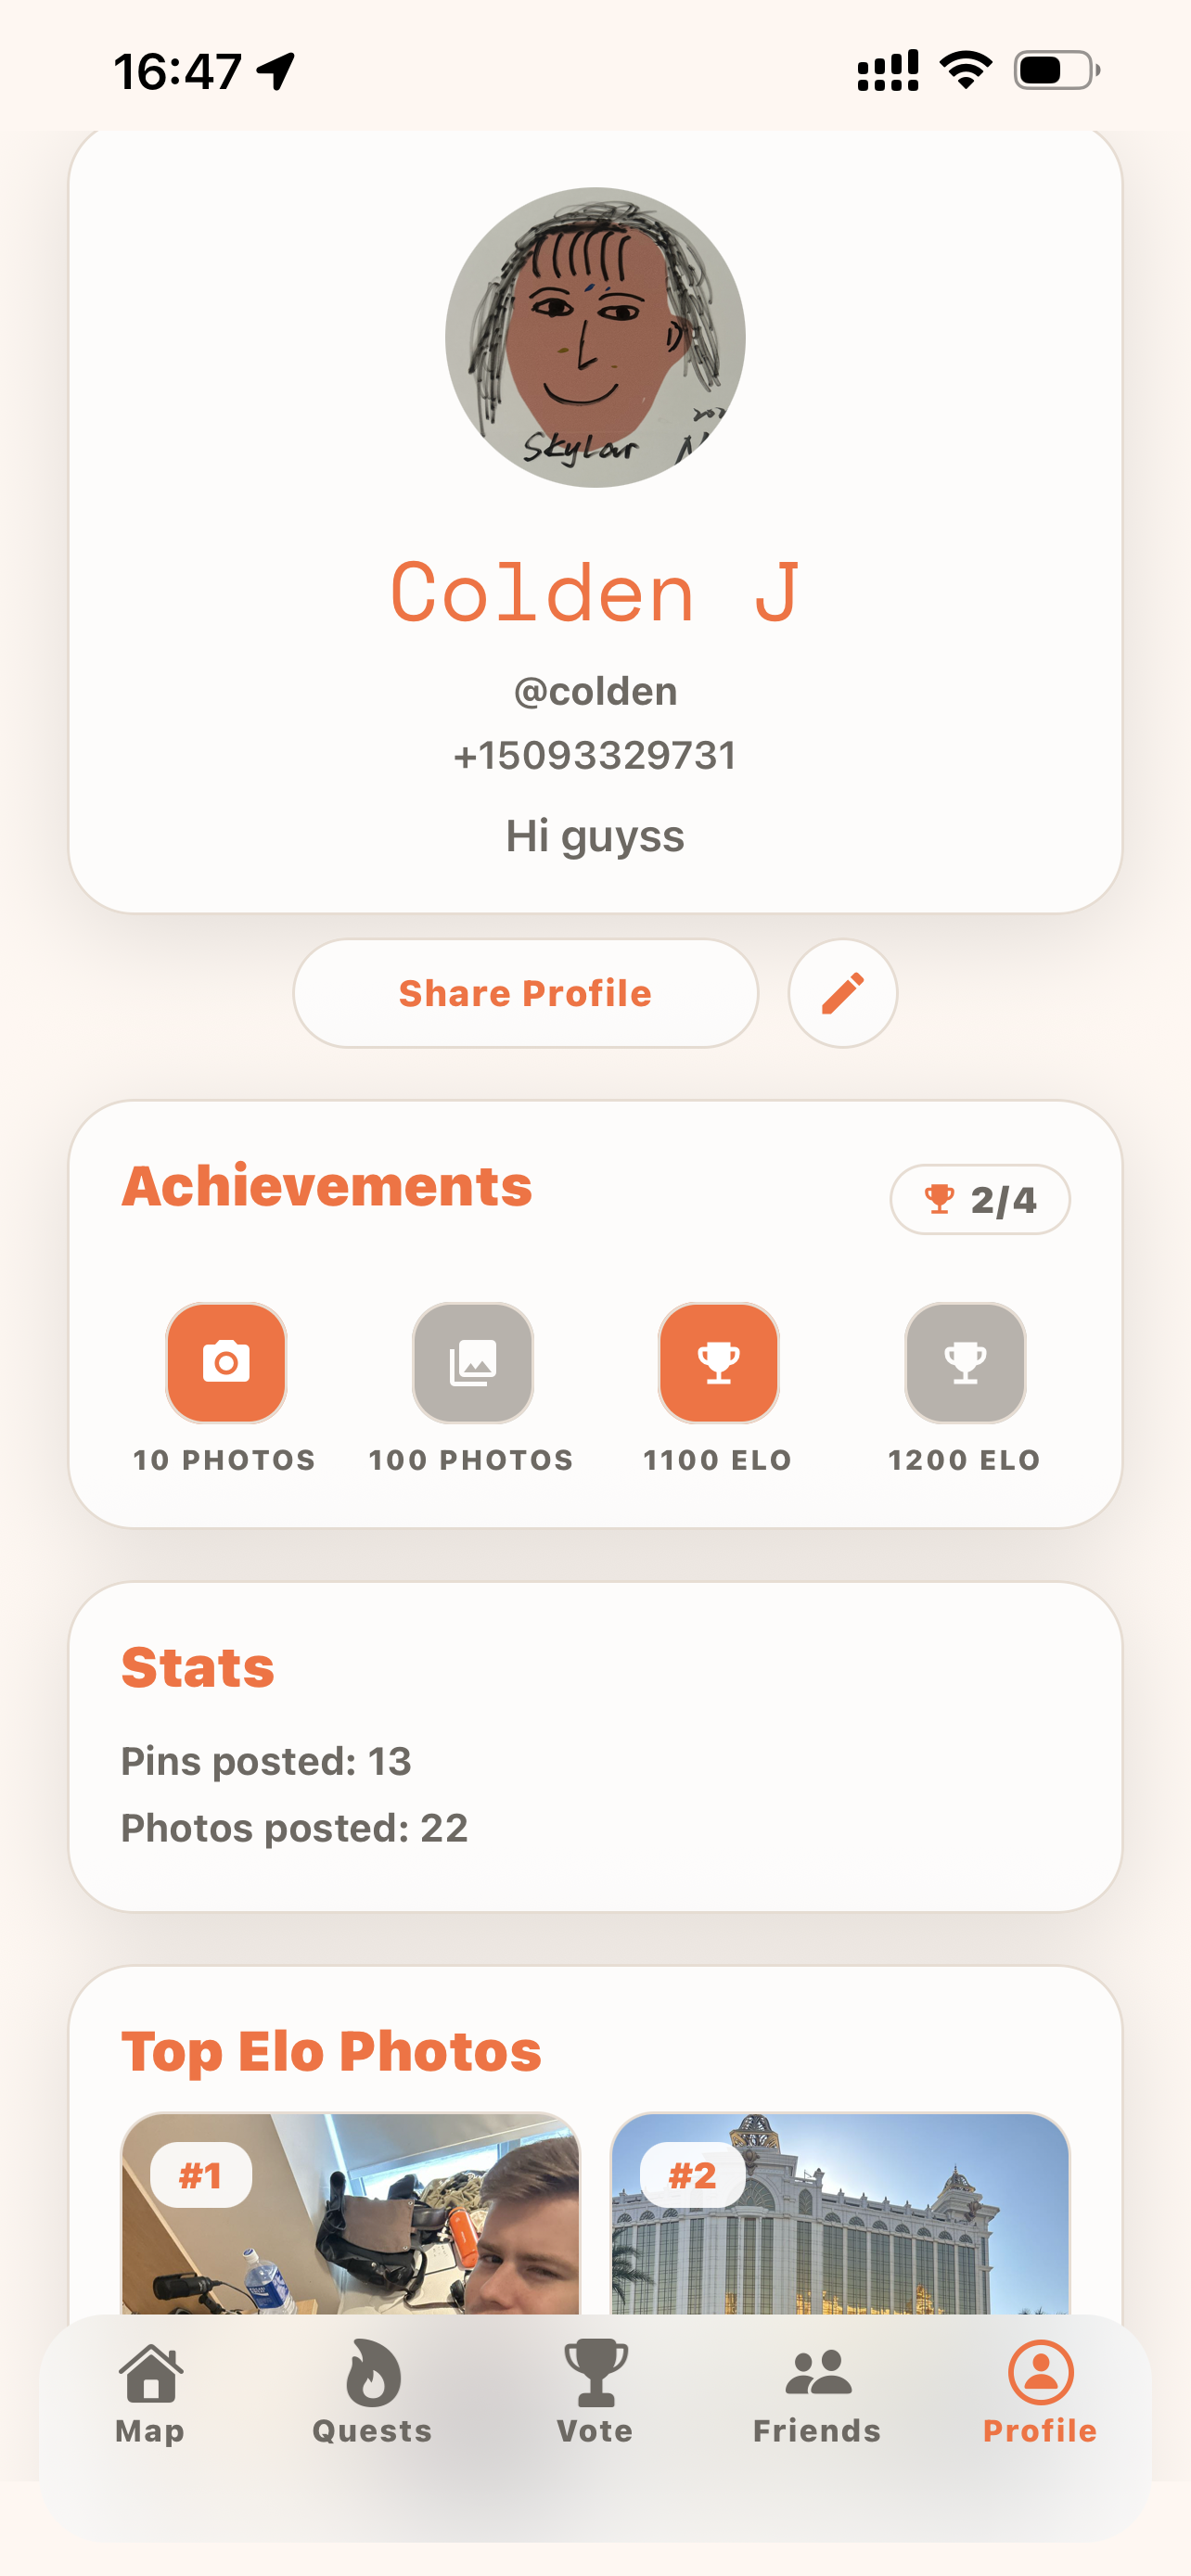
\includegraphics[width=0.48\linewidth]{AppPhotos/Sidequest_Profile.PNG}
  \caption{Profile view. \textit{(User profile page with identity and participation details.)}}
  \label{fig:appphotos-profile}
\end{figure}

\section*{REFERENCES}

{\setlength{\parindent}{0pt}%
\setlength{\parskip}{0.6\baselineskip}%
\newcommand{\mlaentry}[1]{\noindent\hangindent=0.5in\hangafter=1 #1\par}%
\mlaentry{Abidin, Crystal. “Visibility Labour: Engaging with Influencers’ Fashion Brands and \#OOTD Advertorial Campaigns on Instagram.” \textit{Media International Australia}, vol. 161, no. 1, 2016, pp. 86--100. https://doi.org/10.1177/1329878X16665177.}
\mlaentry{BeReal. “BeReal: Your Friends for Real.” BeReal, https://bere.al.}
\mlaentry{Biskjaer, Michael Mose, Peter Dalsgaard, and Kim Halskov. “A Constraint-Based Understanding of Design Spaces.” \textit{Proceedings of the SIGCHI Conference on Human Factors in Computing Systems}, 2014, pp. 2599--2608. https://doi.org/10.1145/2556288.2557342.}
\mlaentry{Bucher, Taina. “Want to Be on the Top? Algorithmic Power and the Threat of Invisibility on Facebook.” \textit{New Media \& Society}, vol. 14, no. 7, 2012, pp. 1164--1180. https://doi.org/10.1177/1461444812440159.}
\mlaentry{de Souza e Silva, Adriana, and Daniel M. Sutko. \textit{Digital Cityscapes: Merging Digital and Urban Playspaces}. Peter Lang, 2009.}
\mlaentry{Deterding, Sebastian, et al. “From Game Design Elements to Gamefulness: Defining ‘Gamification.’” \textit{Proceedings of the 15th International Academic MindTrek Conference}, 2011, pp. 9--15. https://doi.org/10.1145/2181037.2181040.}
\mlaentry{Hemment, Drew. “Locative Arts.” \textit{Leonardo}, vol. 39, no. 4, 2006, pp. 348--355. https://doi.org/10.1162/leon.2006.39.4.348.}
\mlaentry{Instagram. “About Instagram.” Instagram, https://about.instagram.com.}
\mlaentry{Niantic, Inc. “Pokémon GO.” Niantic, 2016, https://pokemongolive.com.}
\mlaentry{Nielsen, Jakob. \textit{Usability Engineering}. Morgan Kaufmann, 1994.}
\mlaentry{Norman, Don. \textit{The Design of Everyday Things}. Revised and expanded ed., Basic Books, 2013.}
\mlaentry{Snap Inc. “Snapchat.” Snap, https://snap.com.}
\mlaentry{Stokes, Patricia D. \textit{Creativity from Constraints: The Psychology of Breakthrough}. Springer, 2005.}
\mlaentry{Zimmerman, John, Jodi Forlizzi, and Shelley Evenson. “Research through Design as a Method for Interaction Design Research in HCI.” \textit{Proceedings of the SIGCHI Conference on Human Factors in Computing Systems}, 2007, pp. 493--502. https://doi.org/10.1145/1240624.1240704.}
}








\begin{figure}[!htbp]
  \centering
  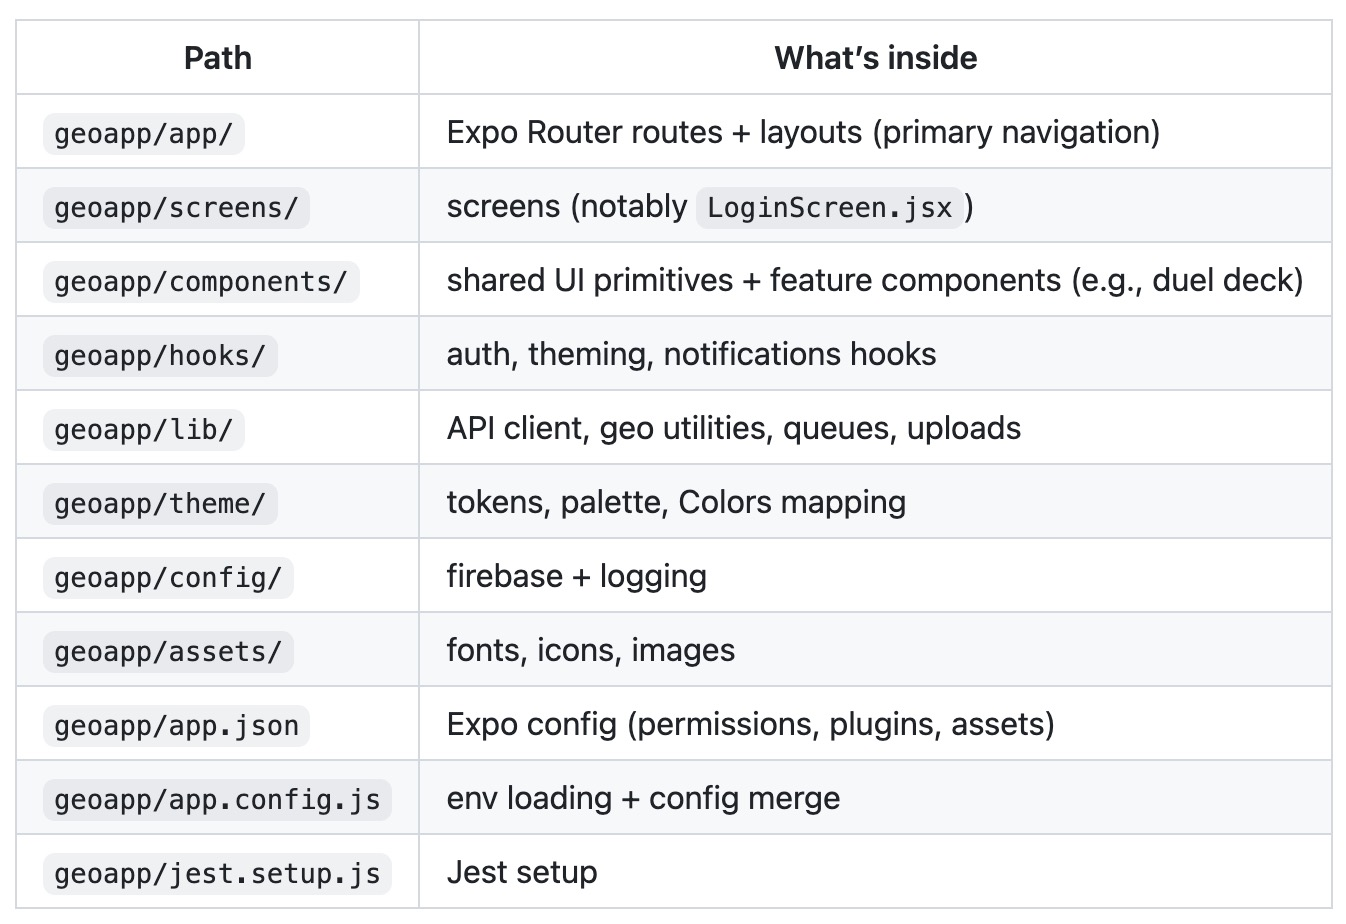
\includegraphics[width=0.7\linewidth]{FrontendStructureChart.jpg}
  \caption{Frontend structure chart. \textit{(High-level organization of the React Native app.)}}
  \label{fig:frontend-structure}
\end{figure}


\end{document}
